\documentclass[oneside]{book}
\usepackage[a4paper, total={6in, 8in}]{geometry}
\usepackage[english]{babel}
\usepackage[utf8]{inputenc}
\usepackage[T1]{fontenc}
\usepackage{cancel}
\usepackage{amsmath}
\usepackage{amsfonts}
\usepackage{dsfont}
\usepackage{listings}
\usepackage{hyperref}
\usepackage{siunitx}
\usepackage{fancyhdr}
\usepackage{textcomp}
\usepackage{makecell}
\usepackage[font=small,labelfont=bf]{caption}
\usepackage{pdfpages}
\usepackage{multicol}
\usepackage[ruled,vlined]{algorithm2e}
\usepackage{soul}
\usepackage[toc, page]{appendix}
\usepackage{float}
\usepackage{wrapfig}
\usepackage{braket}
\usepackage{xcolor}
\usepackage{mathtools}
\usepackage{float}
\usepackage{subcaption}
\usepackage{tgbonum}


%Zotero Bibliography
%\usepackage{apacite}
%\addbibresource{bibliography.bib}


\pagestyle{fancy}
\fancyhf{}
\lhead{\rightmark}
\cfoot{\leftmark}
\rfoot{\thepage}

\setcounter{secnumdepth}{5}

\lstset{
    frame=tb, % draw a frame at the top and bottom of the code block
    tabsize=4, % tab space width
    showstringspaces=false, % don't mark spaces in strings
    numbers=none, % display line numbers on the left
    commentstyle=\color{green}, % comment color
    keywordstyle=\color{red}, % keyword color
    stringstyle=\color{blue}, % string color
    breaklines=true,
    postbreak=\mbox{\textcolor{green}{$\hookrightarrow$}\space}
}

\renewcommand{\lstlistingname}{}% Listing -> Algorithm
\renewcommand{\lstlistlistingname}{Algoritmi}% List of Listings -> List of Algorithms
\renewcommand*{\listalgorithmcfname}{}
\renewcommand*{\algorithmcfname}{}
\renewcommand*{\algorithmautorefname}{}
\renewcommand{\thealgocf}{}
\newcommand{\mathcolorbox}[2]{\colorbox{#1}{$\displaystyle #2$}}
%\renewcommand{\familydefault}{\rmdefault}

% %to use MINTED
% \usepackage{xcolor}
% \definecolor{bgcode}{RGB}{230, 230, 230}  % Bkg color for code block 70 70 70
% \usepackage{minted}
% \usemintedstyle{sas}  % Style for code block
% \usepackage{lmodern}  % To allow bold font inside code block
% \setminted{bgcolor=bgcode}


\title{\Huge\textbf{Computational Human genomics}}

\author{ Maurizio Gilioli \\
  % \small telegram: \href{https://t.me/GiacomoFantoni}{@GiacomoFantoni} \\[3pt]
% \small Github:
% \href{https://github.com/giacThePhantom/computational-microbial-genomics}{https://github.com/giacThePhantom/computationl-microbial-genomics}
}

\makeglossaries

\begin{document}
\maketitle
\tableofcontents

% \input{chapters/} 

% To input a new chapter, you have to copy and past this line
% here above, and use the name of your file without the tex extension. All the
% images included in the file should be inserted in a specific folder inside the
% chapter one.

\graphicspath{{chapters/ThebasicsImages/}}


\chapter{Introduction}
\section{Basic principles} \label{chap: Basics}

\begin{figure}[H]
  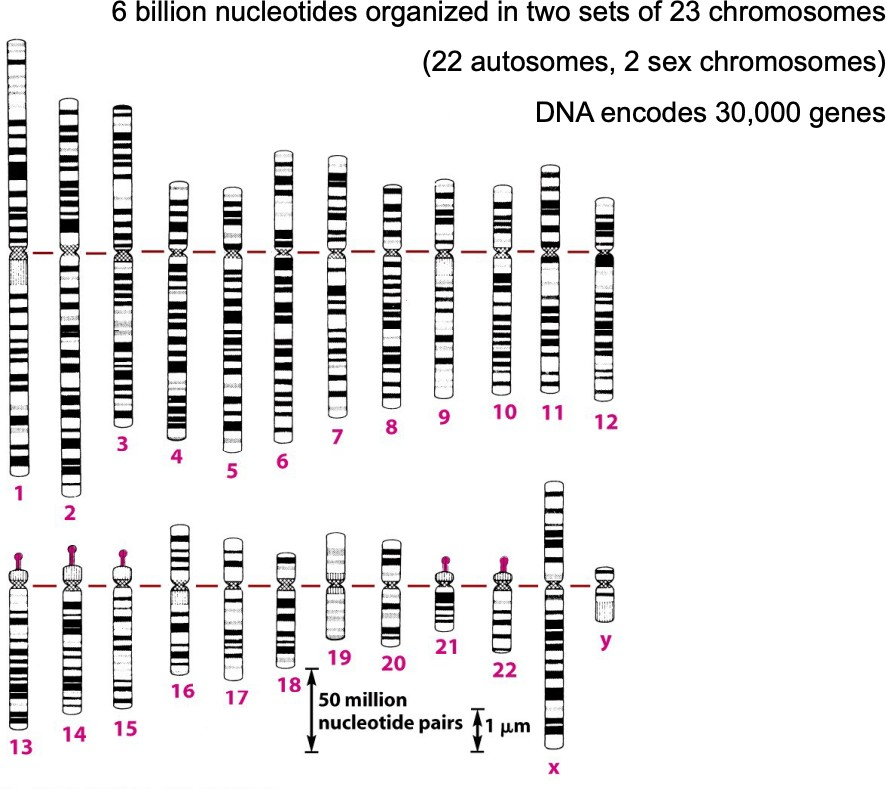
\includegraphics[width=4.32507in,height=3.86281in]{image1.jpeg}
  \centering
  \caption{}
\end{figure}


The words variations, aberrations and lesions are often interchanged.
Aberrations and lesions are mainly used for acquired lesions, instead variations
are mainly used for the inherited ones.

\hypertarget{genetic-make-up}{%
\subsection{Genetic Make-Up}\label{genetic-make-up}}

\begin{figure}[H]
  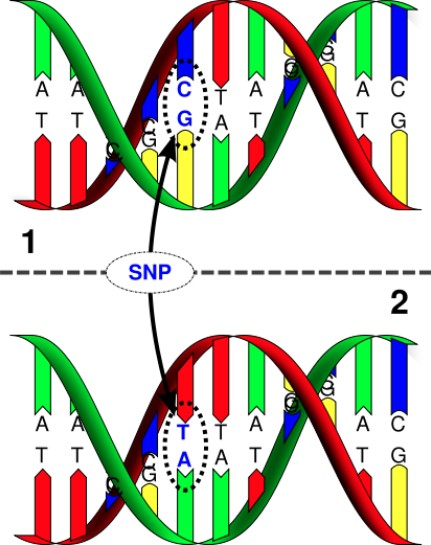
\includegraphics[width=1.97816in,height=2.50248in]{image2.jpeg}
  \centering
  \caption{}
  \label{fig: SNP}
\end{figure}


\textbf{Single Nucleotide Polymorphism} (SNP) is a sequence variation affecting
single bases (point mutations) (figure \ref{fig: SNP}).

The genomes of two unrelated individuals have about 1\% of different bases →
that percentage corresponds to the SNPs.

But looking at the \textbf{Copy Number Variants} (CNV), that difference will be
way higher than only 1\% DNA not present in only two copies, but in multiple,
single or even zero copies (hemizygous loss, homozygous loss). They are less
known as inherited type of variants because they are harder to detect and
identify, but they provide a lot of uniqueness in each of us.


\begin{figure}[H]
  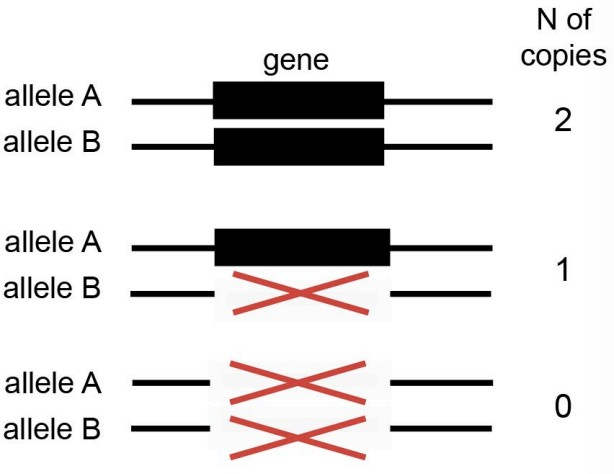
\includegraphics[width=2.93475in,height=2.26167in]{image3.jpeg} 
  \centering
  \caption{}
  \label{fig: SNP}
\end{figure}


Why are SNPs and CNVs so important?

They are responsible of human diversity → genetic changes

Hundreds of CNVs per individual and 20\% of them potentially affect protein-
coding genes

\textbf{Differences} in Genetic Make-up:

Very common variants are variants that are distributed in the population as the
common allele, so that 1/2 of the population has an heterozygous genotype at
that position, 1/4 has an homozygous genotype for one allele and 1/4 has an
homozygous genotype for the other allele.

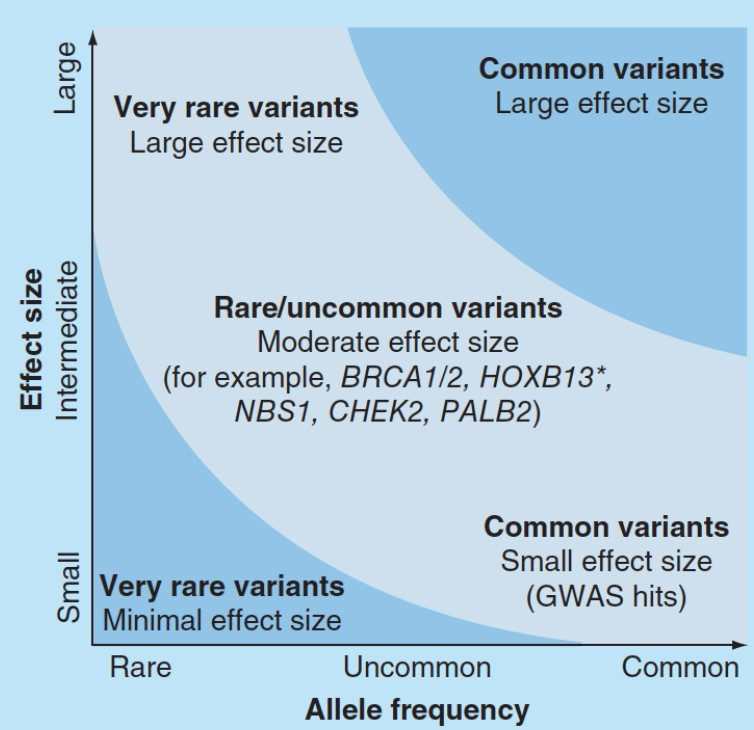
\includegraphics[width=3.9928in,height=3.87812in]{image4.jpeg}

The \textbf{penetrance} is the proportion of individuals carrying an allele (or
a genotype) that also expresses the trait (phenotype) associated with it.
Obviously, penetrance is directly associated with the size of the effect
produced by the variant.

The \textbf{allele frequency} is calculated by dividing the number of times the
allele of interest is observed in a population by the total number of copies of
all the alleles at that particular genetic locus in the population.

The allele frequency is low with very rare variants

Well known variants: BRCA1/2, HOXB13, NBS1, PALB2, CHEK2 → they have moderate
size effects, meaning that all the people who have the variants, have the
disease


\hypertarget{differences-in-genetic-make-up-example}{%
\subsubsection{Differences in genetic Make-Up,
example}\label{differences-in-genetic-make-up-example}}
% article to be read? #TODO


Absorption, distribution, metabolism and elimination (ADME) genetic variants
determine pharmacokinetic variability of certain compounds, influencing the
patients' treatment response. Both common and rare variants are involved.

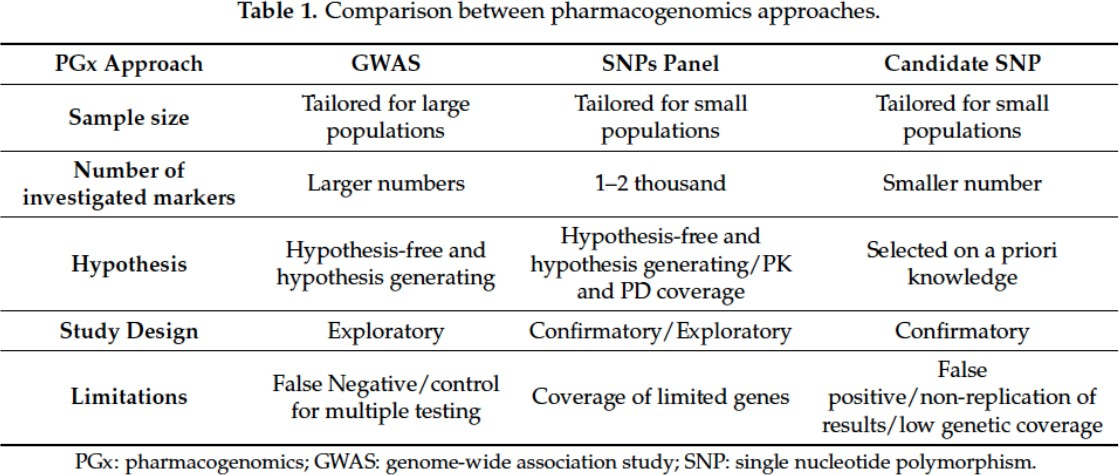
\includegraphics[width=6.18852in,height=2.6224in]{image5.jpeg}

Three main ways to study genetic variants: 

\begin{itemize}
  \item GWAS (genome-wide association study)
  \item SNPs panel
  \item Candidate SNP
\end{itemize}




For example, in terms of hypothesis, if I study all the variants in the human
genome and I query them in a large population, I generate data without
specifying SNP to search. Instead, if I have a very specific hypothesis, for
example I want to query if a SNPs in the CYP gene relates to the conversion of
androgens to estrogens, I don't need to run an GWAS or a wide SNPs panel. I can
query those SNPs because I have an \emph{a priori} hypothesis and I want to test
them.

This type of differential design for an experiment it is not only true for
inherited variants and ADME genes, but also to predisposition to diseases and to
study human tumors.

Precision medicine → treatment (or dosage) of a patient based on their
individual traits: takes into consideration genetic and genomic of the
individual and tumor/disease cells

\begin{itemize}
  \item Drink beer and turn red → ADME gene
  \item Athletes with a deletion of a gene, the steroids were not found in the
  anti-doping tests
\end{itemize}
 

\hypertarget{acquired-dna-aberrations}{%
\subsection{Acquired DNA aberrations}\label{acquired-dna-aberrations}}


Somatic variants are the variants NOT inherited from parents and not transmitted
to offspring. They are:

\begin{itemize}
  \item \textbf{Single Nucleotide Variants} (SNV) are somatic changes of single
  nucleotides present in only certain cells, instead of SNPs that are present in
  all cells of our body.
  \item \textbf{Indels} are changes that involve few nucleotides by INsertion
  and DEletion
  \item \textbf{Rearrangements} are mutations that can involve events like
translocations, inversion, chromothripsis,.. usually these events are caused by
breakage in the DNA double helices a two different locations, followed by a
rejoining of the broken ends to produce a new chromosomal arrangement of genes,
different from the beginning

  \item \textbf{Somatic copy number aberrations} (\textbf{SCNA}) are somatic
changes similar to CNVs. They can be every change related to the number of
copies like loss of a portion of a genome, loss of both alleles, extra copies...
\end{itemize}

\begin{figure}[H]
  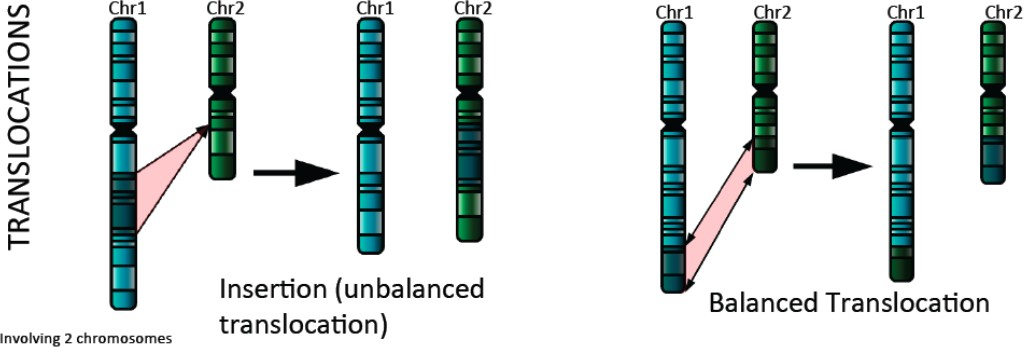
\includegraphics[width=6.1748in,height=2.09646in]{image6.jpeg}\\
  \centering
  \caption{translocations}
  \label{fig: translocations}
\end{figure}

Rearrangements include:

\begin{itemize}
  \item \textbf{Balanced translocation} (figure \ref{fig: translocations}): you conserve the quantity of DNA, there
  isn't any loss or gain.
  
  \item \textbf{Unbalanced translocation}: A genomic portion is translocated
  from a chromosome to another, there is not vice versa.
  
  \item \textbf{Inversions} in only ONE chromosome: everything is normal instead
  in the break points.

  \begin{figure}[H]
    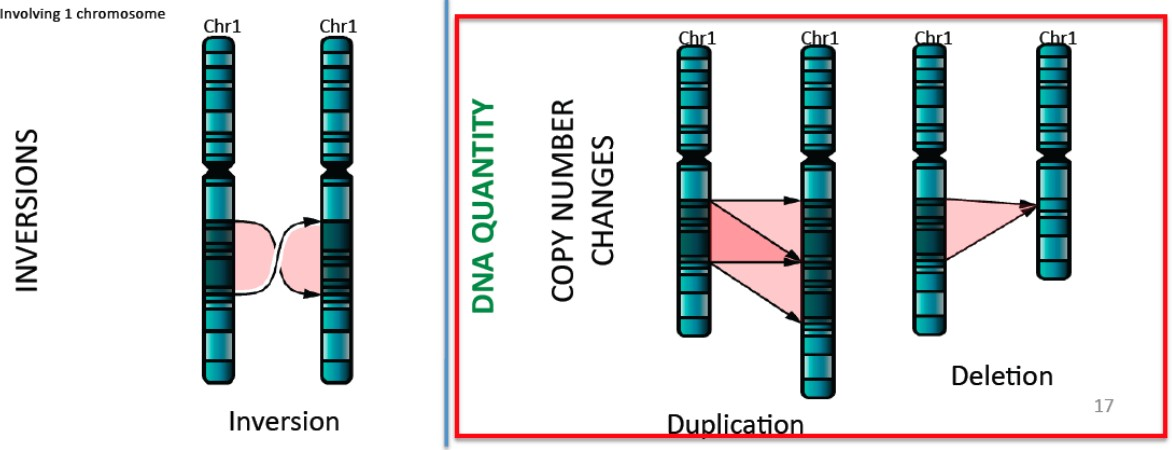
\includegraphics[width=6.22722in,height=2.39062in]{image7.jpeg}
    \centering
    \caption{Duplications inversions and deletions}
    \label{fig: Duplications inversions and deletions}
  \end{figure}

  \item \textbf{Copy number changes:} duplication or deletion. It could happen in
  the same chromosome but also in different chromosomes.
\end{itemize}

Other important modifications:

\begin{itemize}
  \item \textbf{Chromoplexy}: a class of complex somatic DNA rearrangements
  whereby abundant DNA deletions and intra- and inter-chromosomal translocations
  that have originated in an interdependent way occur within a single cell
  cycle.

  \item \textbf{Chromothripsis}: a clustered chromosomal rearrangement in
  confined genomic regions that results from a single catastrophic event,
  usually limited to one chromosome.

  \item \textbf{Kataegis}: a phenomenon that is characterized by large cluster
  of mutations (hypermutation) in the genome of cancer cells. An APOBEC family
  enzyme might be responsible fo the kataegis process.
\end{itemize}
  
\begin{figure}[H]
  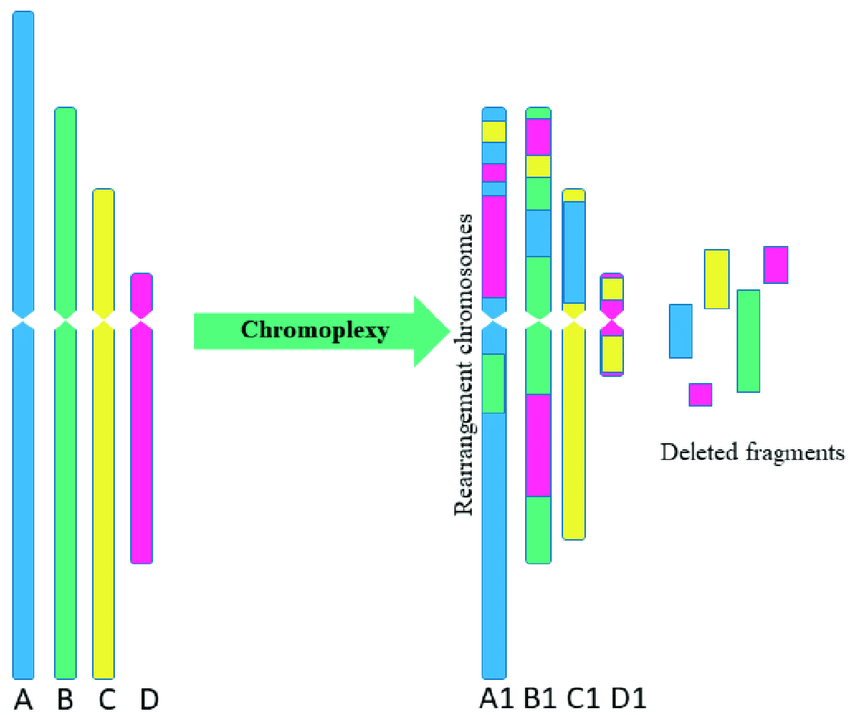
\includegraphics[width=3.81944in,height=3.21433in]{image8.png}\\
  \centering
  \caption{Chromoplexy}
  \label{fig: Chromoplexy}
\end{figure}


When an aberration (clonal) occurs, all the cells will harbour the aberration
and at some point another aberration (subclonal of the other) could appear in
just one cell line. The \textbf{clonal} aberration is present in all the cells,
the \textbf{subclonal} aberration is inherited in just one cell line. Clonality
is an important information that allow us to study evolution.


\hypertarget{experimental-approaches}{%
\section{Experimental approaches}\label{experimental-approaches}}


Experimental techniques to detect variants/aberrations \textbf{prior to NGS}: a
failure because it was very hard to determine the starting points of the
aberrations. %#TODO which tecniques? 

\begin{figure}[H]
  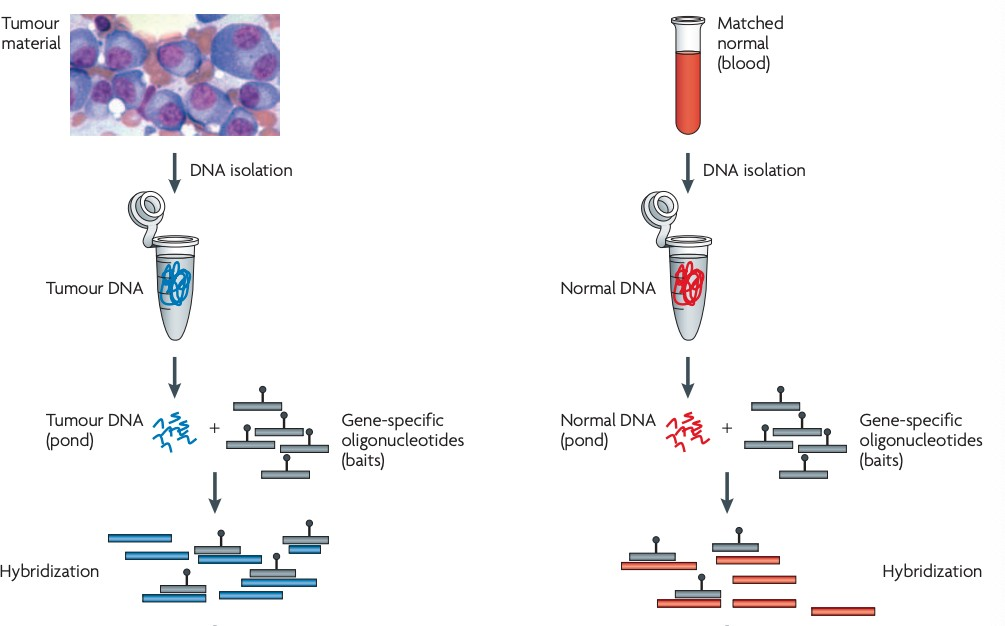
\includegraphics[width=6.18343in,height=3.84729in]{image9.jpeg}
  \centering
  \caption{Meyerson et al. 2010, ``Advances in Understanding Cancer Genomes
  through Second-Generation Sequencing.'', Nature Reviews Genetics,
  \url{https://doi.org/10.1038/nrg2841}}
  \label{fig: DNA variants}
\end{figure}

Bulk of tumor tissue/cells from the blood procedure (figure \ref{fig: DNA variants}):


\begin{enumerate}
\def\labelenumi{\arabic{enumi})}
\item
  DNA isolation.
\item
  Gene-specific oligonucleotides (\textbf{baits}) that get hybridized onto the
  tumor DNA → the baits have a tag that allows them to be isolated.
\item
  The DNA does get fragmented.
\item
  The captured DNA is eluted and prepared into sequencing libraries.
\item
  Sequencing.
\item
  Aligned to the bait sequences.
\end{enumerate}


We repeat the procedure for healthy cells of the same individual in order to
\textbf{detect somatic mutations}.

\begin{figure}[H]
  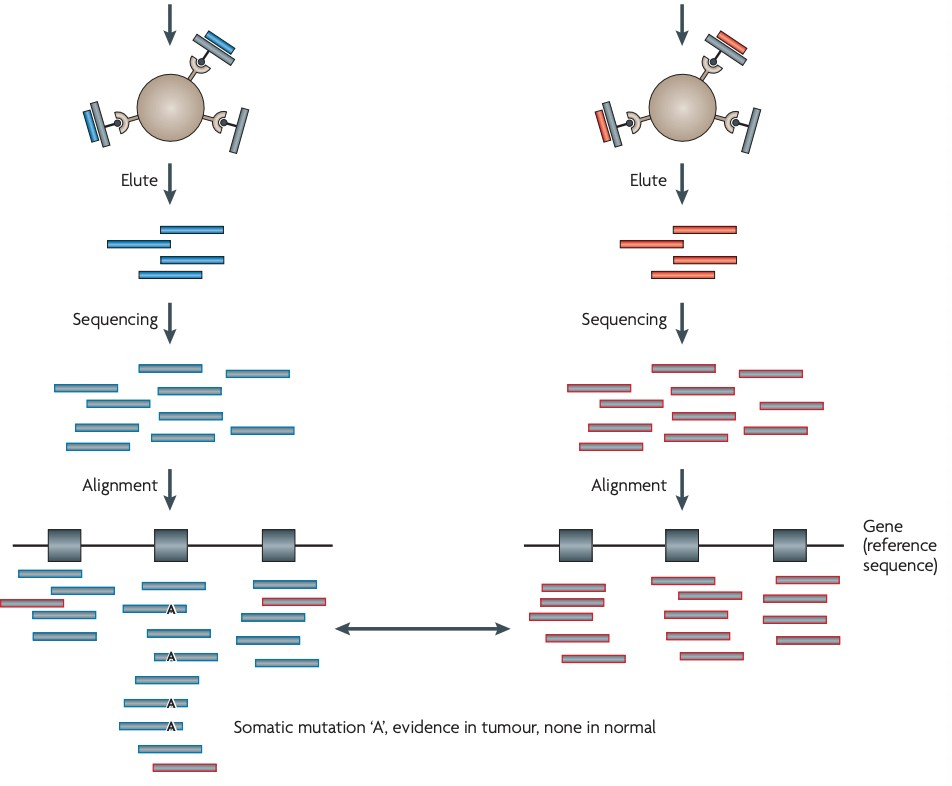
\includegraphics[width=6.14828in,height=5.07625in]{image10.jpeg} \label{fig:
  DNA cancer variants detection}
  \centering
  \caption{Beads capture}
\end{figure}


We sequence baits because is way cheaper (exons of 50 bases instead the whole
genome)

After fragmentation procedure, before adding the adapters, we can choose between
two different sequencing approaches \ref{fig: sequencing methods}:\\



\includegraphics[width=0.75\textwidth]{image11.png}\\ \label{fig: sequencing
methods}
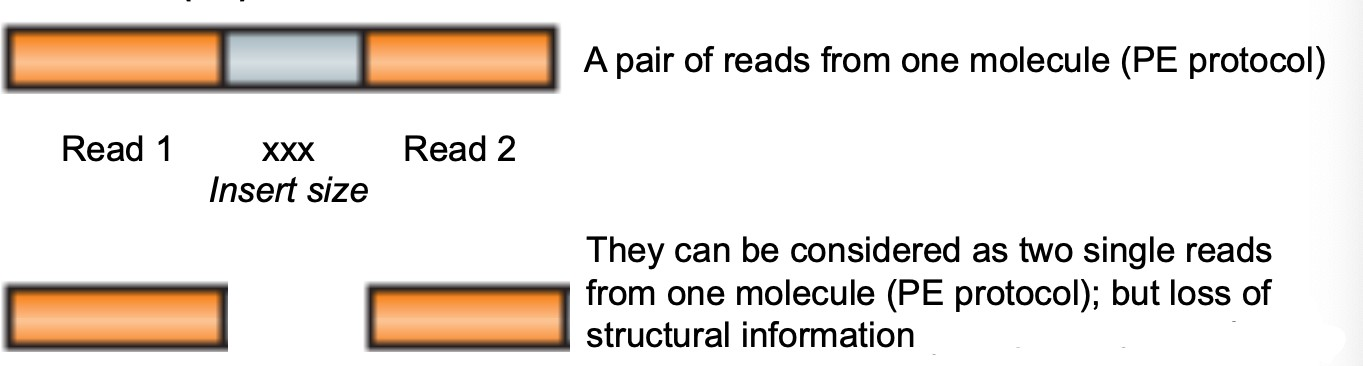
\includegraphics[width=0.75\textwidth]{image12.jpeg}

\begin{itemize}
  \item \textit{\textbf{Paired End (PE) sequencing}}

  You will sequence only one part of a molecule (length of 150 bp → based on the
  power of the sequencing machine we are using). You will know exactly 150 bp
  for every molecule you sequence, but you lose information (the second end of
  the pair).

  \item \textit{\textbf{Single End (SE) sequencing}}
  
  You information about the length of the DNA portion between the ends. It's
  more expensive, but:

  \begin{itemize}
    \item
      it gives information about the localization of the molecule
    \item
      you can treat each end as single read
    \end{itemize}

\end{itemize}


\subsection{Information after reads mapping over reference genome}

\begin{figure}[H]
  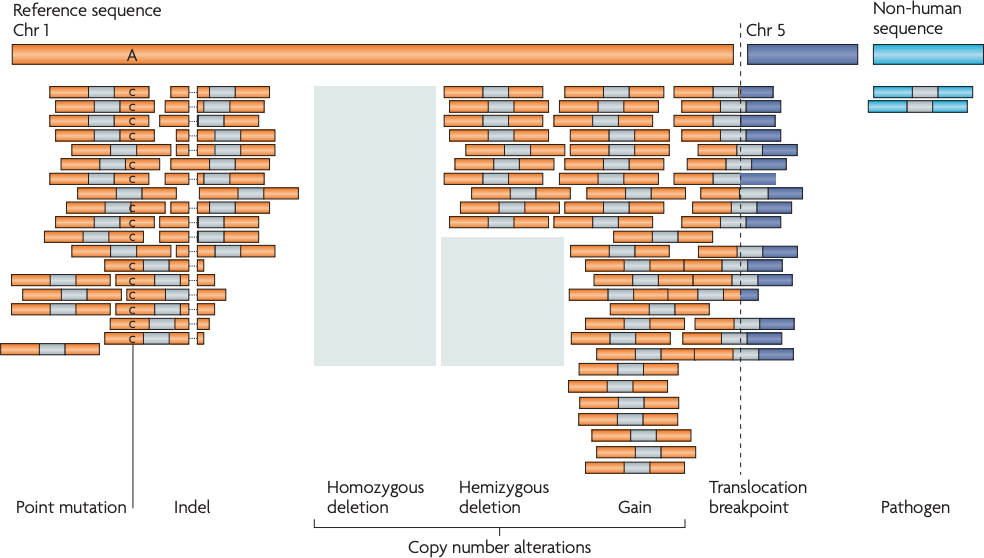
\includegraphics[width=6.16003in,height=3.4875in]{image13.png}
  \centering
  \caption{In the following picture: a view of reads that are mapped against
  reference genome and what we would look if we have any of the variations that
  we mentioned}
\end{figure}

Following the mapping of the reads over the reference genome, different types of
genomic alteration/information can be detected:

\begin{itemize}
  
  \item You can clearly identify \textbf{point mutations}. If a point mutation
  is present in the molecule that you sequenced and present on both alleles of
  the genome, it can be seen in all the reads very clearly.
  
  \item You might see \textbf{indels} (shown here by a dashed line). You will
  see a little space because the reference genome has more nucleotides than the
  sequenced molecule.
  
  \item If you have \textbf{homozygous deletion}, you don't see anything mapped
  in that portion: there's no DNA. Doesn't matter if SE or PE.
  
  \item If you have \textbf{hemizygous deletion}, you see the read mapped to
  that portion where the hemizygous deletion is sitting, that is more or less
  proportional to half of the reads that you have in regions where you don't
  have a copy number change. Doesn't matter if SE or PE.
  
  \item If you have \textbf{gain}, what you get is higher number of reads
  aligned against that part of DNA, underlying the fact that the molecule you
  sequenced has extra DNA for that portion of reference genome. Doesn't matter
  if SE or PE.

  \item \textbf{Translocation breakpoint} are very important!! You will have one
  end mapping the chr1 and the other end mapping the chr5. Those two ends come
  from the same molecule of the \emph{target cell} (the cell we sequenced), it
  means the cell has a translocation between chr1 and chr5. Without the PE
  protocol you cannot have this result.
  
\end{itemize}

\begin{figure}[H]
  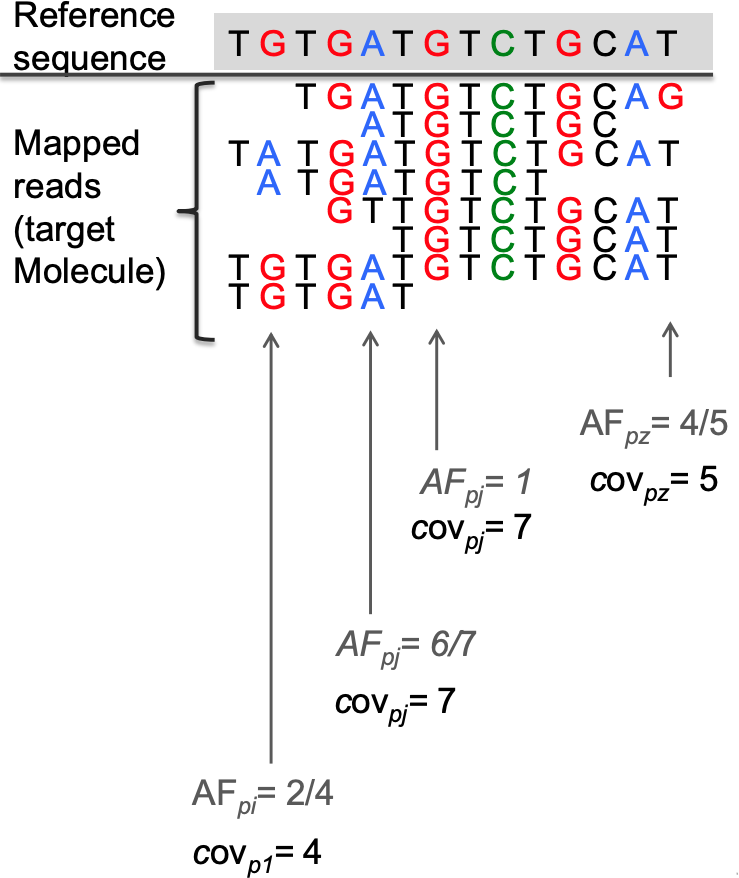
\includegraphics[width=0.4\textwidth]{image14.png}
  \centering
  \caption{View of sequence alignment} \label{fig: coverage and allele
  frequency}
\end{figure}


The \textbf{local coverage} (cov) as shown in figure \ref{fig: coverage and
allele frequency} at position $i$ is the number of reads that span $p_i$.

The \textbf{allelic fraction} (AF) as shown in figure \ref{fig: coverage and
allele frequency} at position $i$ is the proportion of reads that supports the
reference base in $p_i$ (= the reference or the alternative allele).

\subsection{Whole Genome Sequencing Coverage}

\begin{equation} \label{eq: coverage formula}
  cov = \frac{L \dot N}{G}
\end{equation}

where:

\begin{itemize}
\item
  \textbf{L} is the read length.
\item
  \textbf{N} is the number of mapped reads.
\item
  \textbf{G} is the haploid human genome length.
\end{itemize}


This is super important because it saves us time and money when we design an
experiment. When you design an NGS experiment, you should know before what is
the type of coverage you need to answer the question you wanna ask with your
experiment. For example, if you want to look at the genotype of SNPs (inherited
polymorphisms at single side), you don't really need a coverage which is above
$10$ or $15$. So you can design your experiment in order to have an average
coverage equal to $10$ or $15$. To do that, you reverse the equation and count
how many reads you need to generate to achieve that goal. \\

\textit{N.B.}: The number of mapped reads will be always lower of the number of
reads generated by the machine (than the expected). There might be duplicates
that you might not be able to use because there might be reads that have a
quality below the threshold you intend to use.


\hypertarget{difference-between-sequence-coverage-and-physical-coverage}{%
\subsubsection{Difference between sequence coverage and physical
coverage}\label{difference-between-sequence-coverage-and-physical-coverage}}


A graphic view of how \textbf{SE (Single End Sequencing)} or \textbf{PE (Paired
End Sequencing)} can be used:

\begin{figure}[H]
  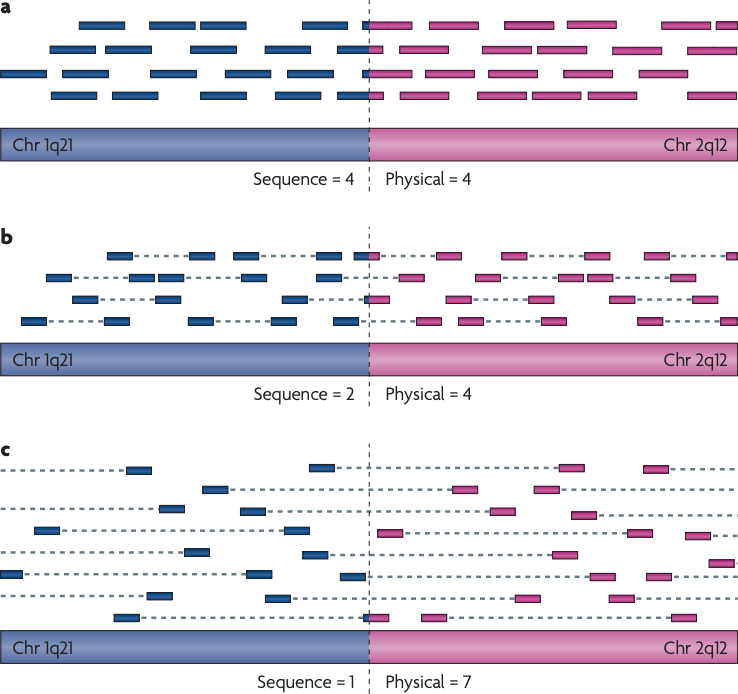
\includegraphics[width=0.65\textwidth]{image15.png}
  \centering
  \caption{Panel A - SE protocol; Panel B - PE protocol; Panel C - PE protocol}
  \label{fig: physical coverage vs coverage}
\end{figure}

Three different scenario are depicted that vary in the length of the DNA
fragments that are sequenced. \textbf{Sequence coverage} represents the number
of sequenced reads that cover the site; this affects the ability to detect point
mutations. \textbf{Physical coverage} measures the number of fragments that span
the site; this affects the ability to detect the rearrangements, based on paired
reads that map to different chromosomes. It is a way informative type of
coverage: for instance for translocations, deletions $\dots$

In Paired End sequencing protocols, the physical coverage is always higher than
the sequence coverage. Choosing the method illustrated in panel 3 (figure
\ref{fig: physical coverage vs coverage}).

Making estimation of intended coverage and observed coverage is very important.
Below I will report an example:\\


\noindent \underline{\textbf{Example coverage observation:}}\\

In these panels were designed to sequence a set of $10$ genes that the
researchers were interested in for prostate cancer. They designed this panel,
sequenced cell lines on this panel and observed the following points

\begin{itemize}
  \item On $x$-axis: the genomic location
  \item On $y$-axis: the local coverage (amplicon median coverage = each bar
  represents the local coverage of about 30 bp)
\end{itemize}

The different colors represent the different genes


\begin{itemize}
  \item \textbf{$1^{st}$ panel}: Local coverage (pile-up) of selected areas
  (targeted sequencing assay): 7 genes

  \begin{itemize}
    \item + 1 multi-gene region (T2ERG). Alternate colors indicate targeted
    areas The barplot show a single sample (LnCaP cell line; cancer cell line)
    data.
    \item Apparent \textbf{deletion} of PTEN (monoallelic deletion) because the
    local coverage of PTEN is significantly lower than the one from other genes.
  \end{itemize}
  
  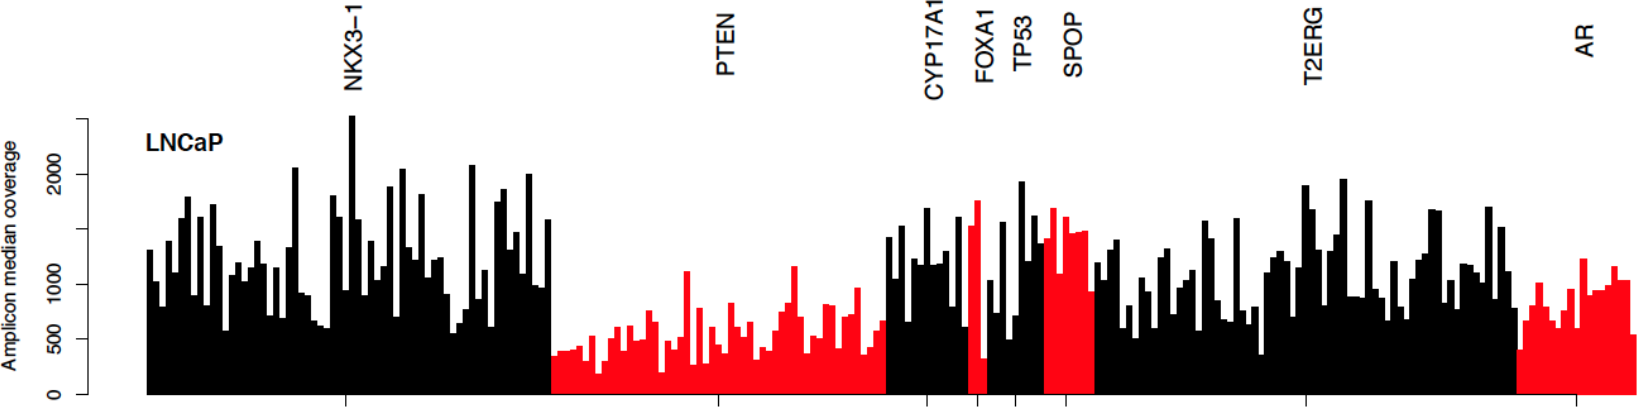
\includegraphics[width=6.13481in,height=1.52625in]{image16.png}

  \item \textbf{$2^{nd}$ panel}: Local coverage (pile-up) of selected areas
  (targeted sequencing assay): 7 genes

  \begin{itemize}
    \item + 1 multi-gene region.
    \item Monoallelic deletion and partial biallelic deletion of PTEN because
    one portion is deleted and one not. PTEN has a \textbf{partial homozygous
    deletion}.
    \item The PC3 cell line shows a little bit of gain in the gene SPOP and
    FOXA1.
    \item The average coverage for the PC3 cells is approximately the same as
    the previous sample.
  \end{itemize}
  
  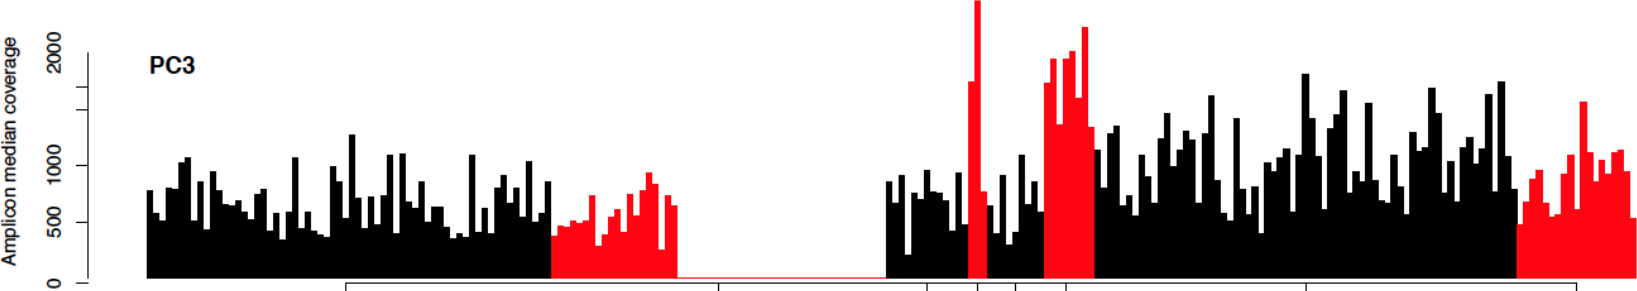
\includegraphics[width=6.15327in,height=1.09125in]{image17.png}

  \item \textbf{$3$rd panel}: 
  
  \begin{itemize}
    \item There's no homozygous deletion but has a high level
    \textbf{amplification} of one area \emph{absorbs} all the reads. Massive
    amplification of the Androgen Receptor (AR) → error: because it inhibits the
    sensitivity of detecting copy number changes in any other gene, the signal
    is excessively intense.
    \item When designing a panel we must pay attention and make sure that we
    don't have potential aberration that basically will draw all the attention
    of your experiment and leave you without information or \textbf{sensitivity}
    in all other regions.
    \item  It's easy to \underline{increase the experimental coverage (i.e. the
    sequence depth) at later point}. Provided tour original sample/library is
    still available, you can perform another run of sequencing and then combine
    the output from different runs.
  \end{itemize}

  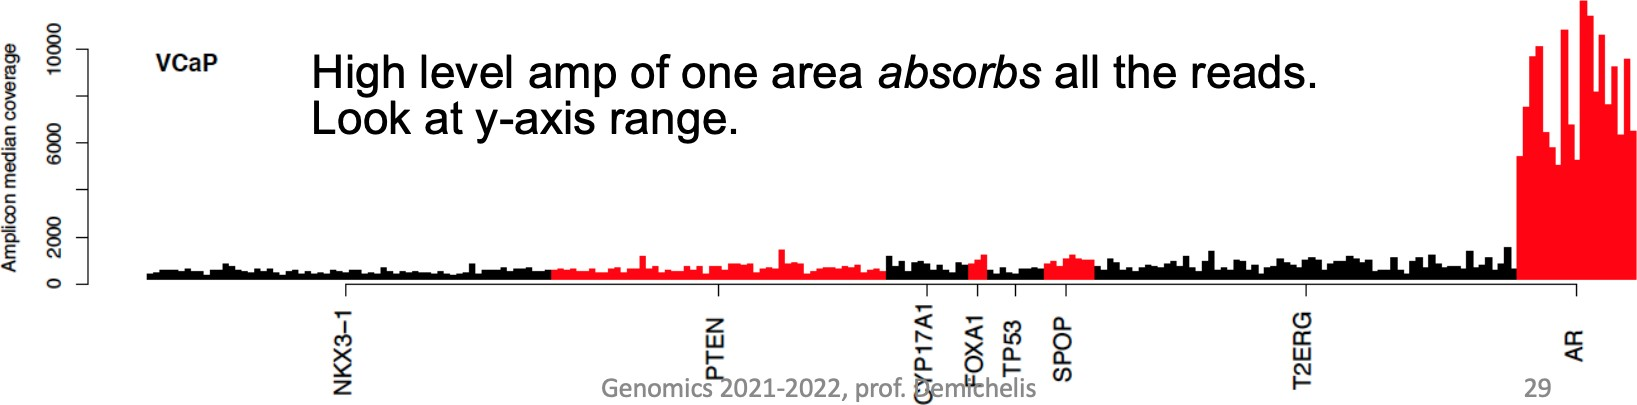
\includegraphics[width=6.17134in,height=1.51875in]{image18.jpeg}
\end{itemize}


\hypertarget{note-that-this-isnt-possible-with-array-based-technologies.}{%
\subsubsection{Note that this isn't possible with array-based
technologies.}\label{note-that-this-isnt-possible-with-array-based-technologies.}}


What are the limiting factors of NGS DNA-seq experiment, in any?

Repeated regions due to \textbf{short reads}

What is the problem of short sequencing on long genome?

\begin{itemize}
  \item Complexity regions
  \item GC content
\end{itemize}
% non ho capito questo commento #TODO


\hypertarget{the-reference-sequence-of-the-human-genome}{%
\section{The reference sequence of the human
genome}\label{the-reference-sequence-of-the-human-genome}}


Many years ago, some people claimed that the entire human genome was sequenced
but it wasn't true at all. There were still unknown or missing regions. In 2022
we finally have the complete human reference genome sequence.

But we need to consider the polymorphisms, there is no \textbf{unique} genome.
How to integrate them into a single reference genome? There is a consortium that
deals with these problems. They assemble a reference genome that reflects the
most common (in the whole population) sequences at each position of the human
genome, but also tracks information of everything that is polymorphic. So that
we can use the latest release of what they built as reference genome and then
use databases to learn about all the polymorphic sites and all the features of
every polymorphic variants.

Genome Reference Consortium:
(\href{https://www.ncbi.nlm.nih.gov/grc/human}{Genome Reference Consortium
link}) where you can find different versions of human reference genome

UCSC Genome Browser on Human: (\href{http://genome-euro.ucsc.edu/}{UCSC link})

where you can upload different versions of the reference


\hypertarget{interpreting-pair-orientation}{%
\subsection{Interpreting pair orientation}\label{interpreting-pair-orientation}}


Using IGV (Integrative Genomics Viewer) (see chapter \ref{chap: IGV} for more
details)

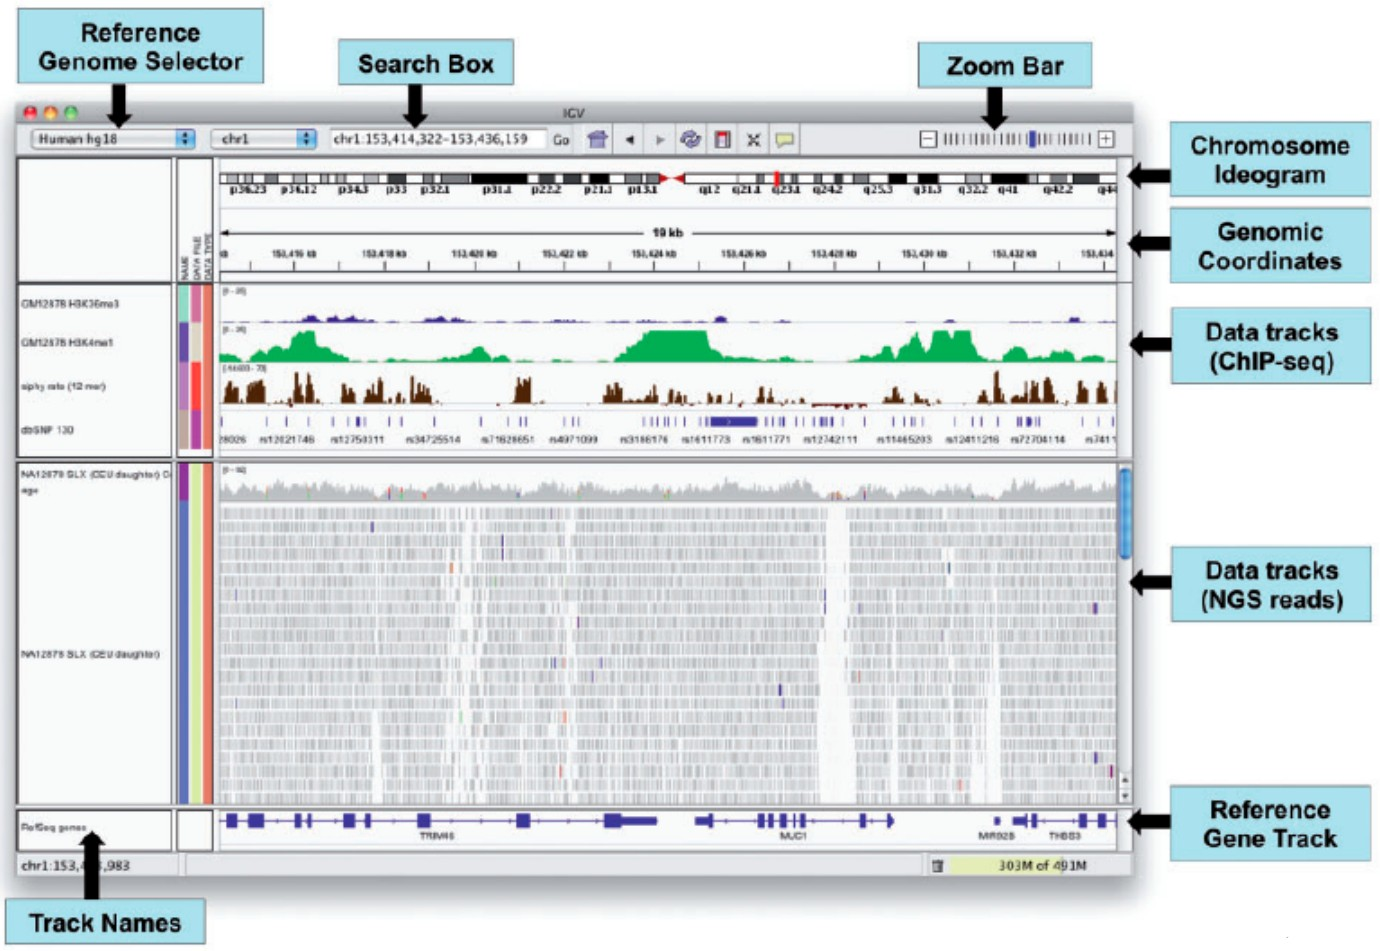
\includegraphics[width=6.32631in,height=4.35875in]{image19.jpeg}

The main characteristic of IGV is that it is a main view viewer: all the
information are in one window.

On the x-axis there's the genome coordinates at the top, the reference genome at
the bottom (we can select the reference genome we prefer).

Along with the data tracks there is the local coverage of the kb shown in the
window (of the sample we are looking at).

You can get any information you want of any single read that you are uploading,
very useful to see difference from the reference genome because every aberration
or whatsoever is highlighted by a different color in the local coverage of a
nucleotide base. Moreover, it gives information about the quality of the read
and the bases, if you have a PE protocol, it tells you also information about
the PE for each of them.

The \textbf{orientation} of paired end can be used to detect structural events,
including: 

\begin{itemize}
  \item Inversions
  \item Duplications
  \item Translocations
\end{itemize}


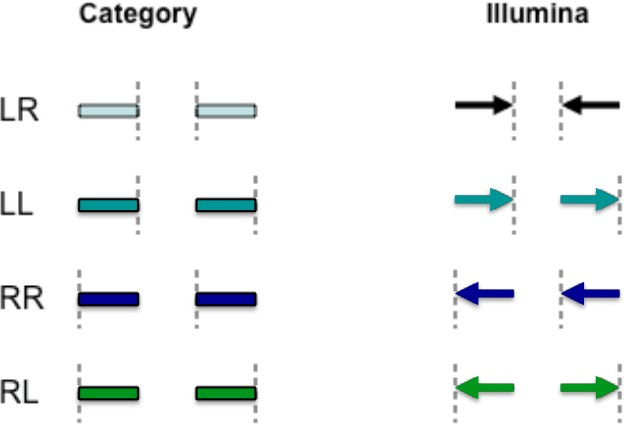
\includegraphics[width=3.89062in,height=2.65in]{image20.jpeg}


\hypertarget{inversion}{%
\subsection{Inversion}\label{inversion}}


A segment of DNA is inverted\\


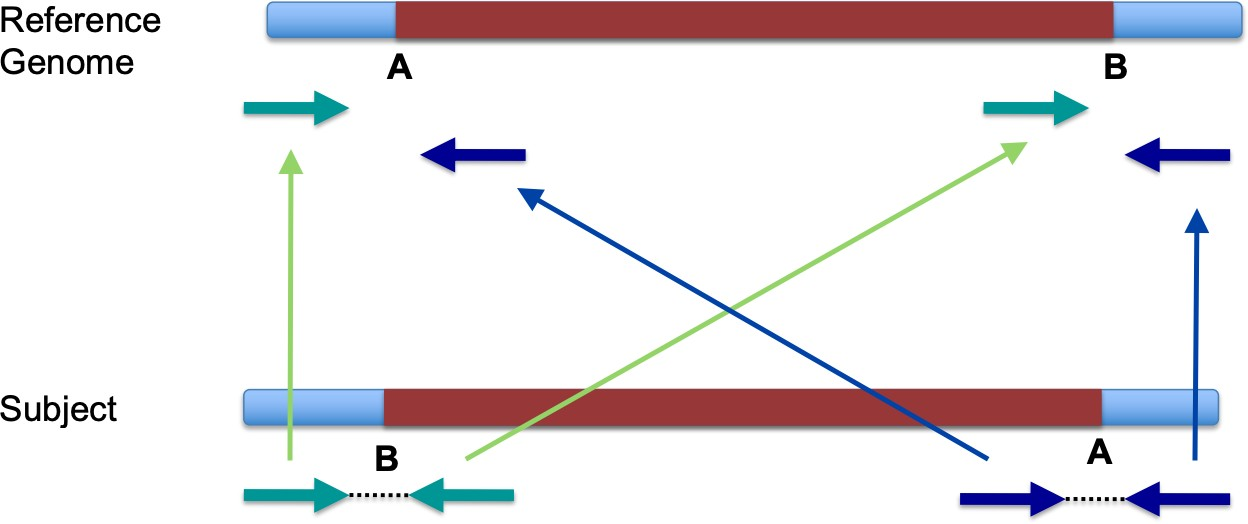
\includegraphics[width=5.85745in,height=2.45625in]{image21.jpeg}


The most important pairs are the ones that stand between junctions because they
are the most informative ones.

Here one end mapped where it was on the reference genome while the other end
reversed its orientation.\\

In IGV:\\


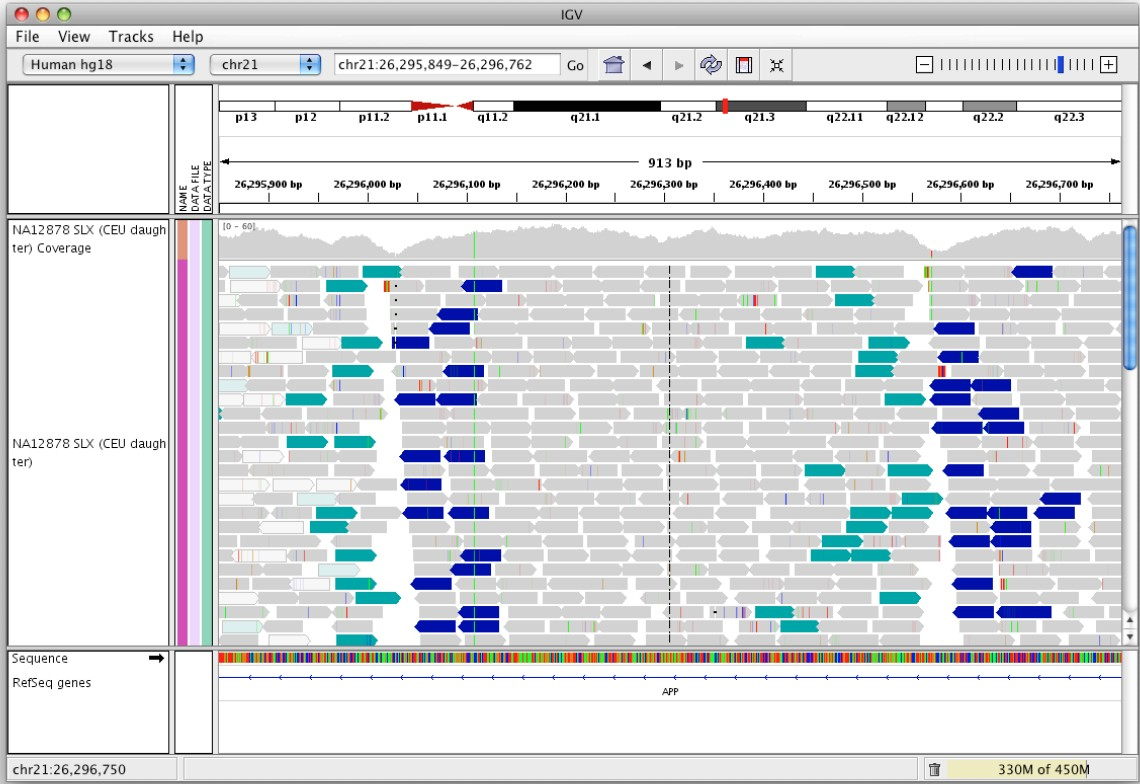
\includegraphics[width=6.29861in,height=4.32833in]{image22.jpeg}


Information that help us:

\begin{itemize}
  \item The \textbf{insert size} from the target molecule (= the subject) is way
  longer. For all the pairs that are at the breakpoint, the insert size is
  different from the expected.

  \item The \textbf{orientation} is different.
  
  \item If you look at the local coverage, you can see a \textbf{drop} in two
  points: at the breakpoints. The reads that are mapping the junctions cannot
  map the reference genome because the breakpoint sequence is altereed in the
  reference genome. So, if we have an inversion in only one of the two alleles,
  then the reads coming from the allele with the inversion will not contribute
  to the local coverage at the breakpoint. The contribution to the local
  coverage will come only from one allele.
\end{itemize}


Moreover, we can notice that the coverage on the middle part does not change
significantly from the coverage on the sides.

When you align reads against a genome, you can \underline{allow for a certain
mismatches or partial alignment}. So, if you impose certain thresholds to your
aligner, you can also say that if there are reads that align for 80\% and have
20\% of sequences misaligned, you align them in any case. So you will have reads
that are correct up to the breakpoints and the browser will shows the mismatches
beyond the breakpoint. So, you can have a partial drop of coverage because you
allow mismatches in your alignment.


\hypertarget{tandem-duplication}{%
\subsection{Tandem duplication}\label{tandem-duplication}}


A segment of DNA is duplicated and inserted in the target molecule adjacent to
the original one.


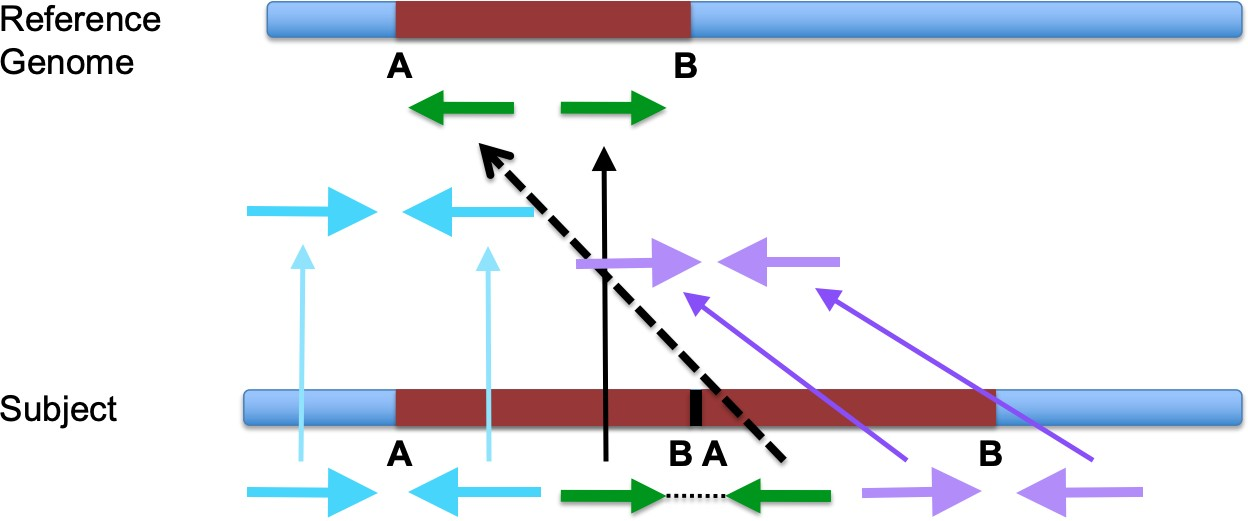
\includegraphics[width=6.1113in,height=2.55073in]{image23.jpeg}\\

So, as result, the orientation instead of going inward goes outward.\\

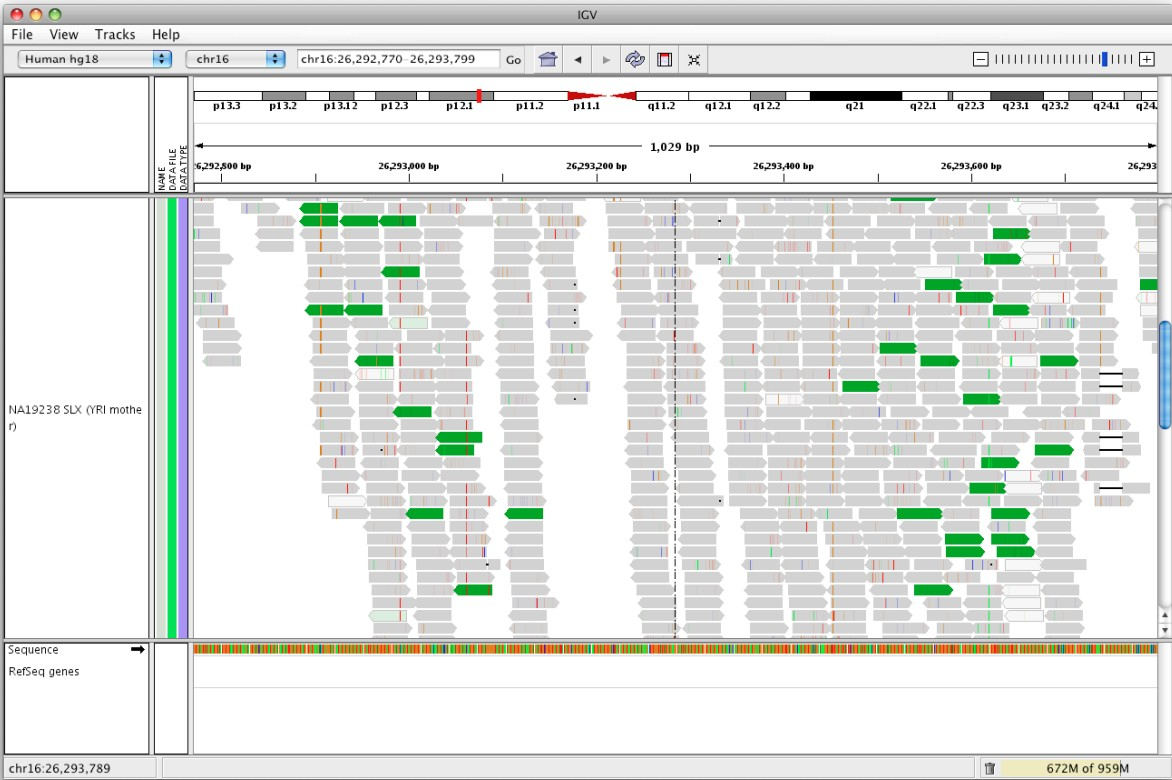
\includegraphics[width=6.22598in,height=4.14375in]{image24.jpeg}\\

\emph{What do you expect to see from coverage?} We will have a gain in coverage
that is proportional to the extra copy. We need to pay attention to the double
because it is a double contribution of that allele, but if a tandem duplication
happens only in one allele and the other allele has his own one copy, then the
local coverage corresponding to the tandem duplication will be 3/2 of the
expected coverage.\\

If you have a read that maps BA, do you expect to see it in the mapped reads?
Partial mapping. As we said before, if you allow your mapper to have some
mismatches of a certain percentage of bases from your reads, you can still see
some coverage contributed on one end of the segment and mismatches on the other
side.
% #TODO da riscrivere

For what concern the \underline{junctions}, you shouldn't see any difference of
coverage because that sequence exists only once in the target molecule. The
local coverage increases only in correspondence of the segment AB.


\hypertarget{inverted-duplication}{%
\subsection{Inverted duplication}\label{inverted-duplication}}


The duplication is inverted but it's not located near the original fragment, but
somewhere else.

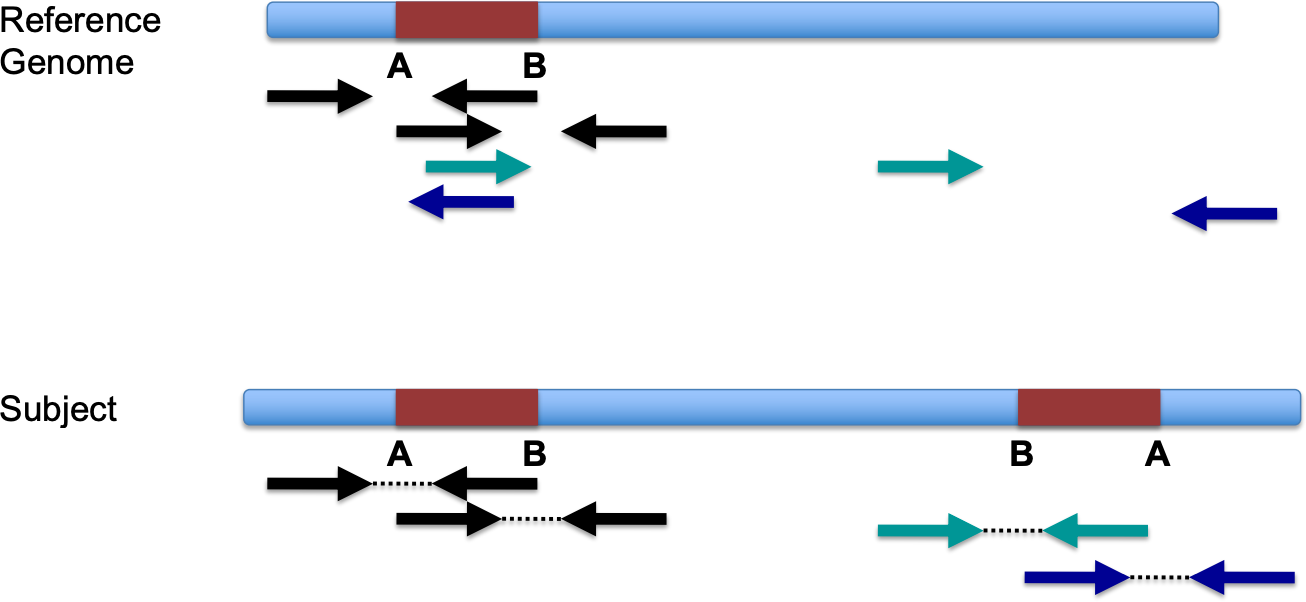
\includegraphics[width=6.11483in,height=2.82187in]{image25.png}\\


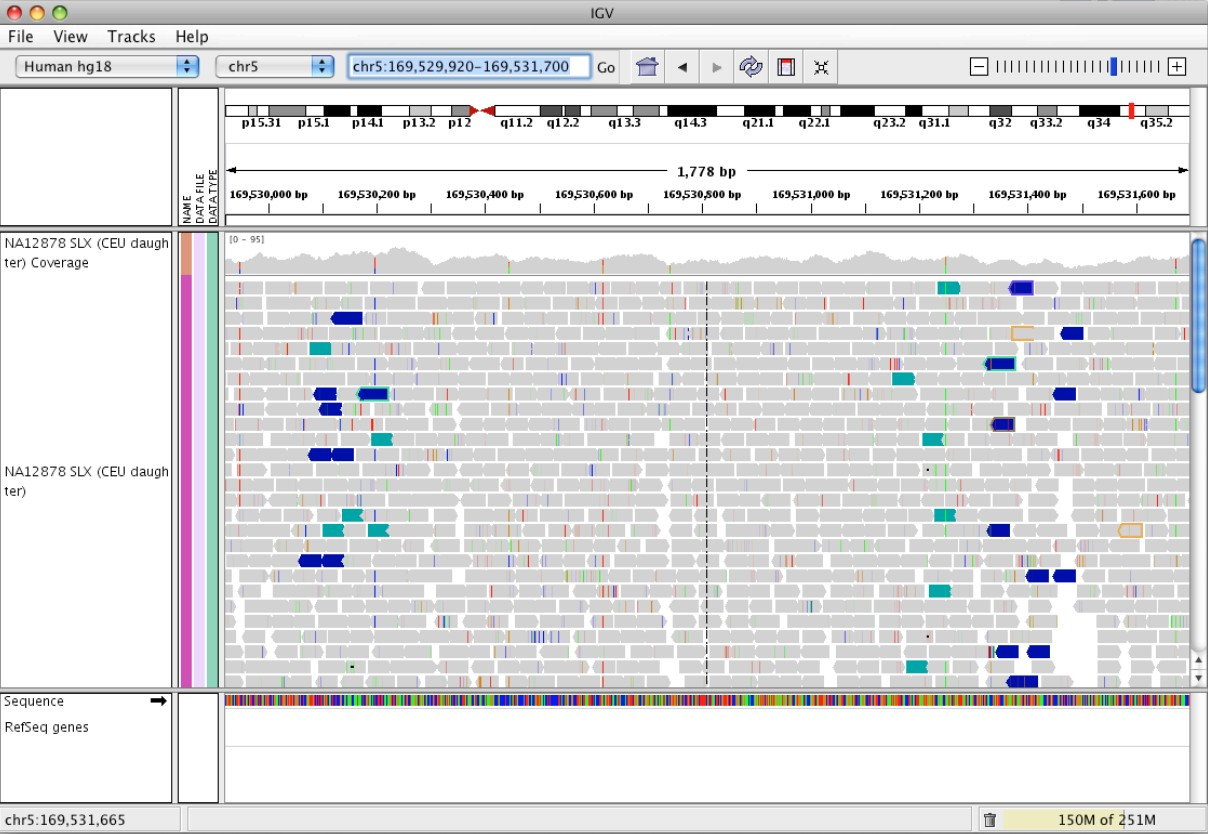
\includegraphics[width=6.29059in,height=4.34375in]{image26.jpeg}\\


There is a gain of coverage in the duplicated region and a tiny drop in the
break points where the sequence exists in only one allele.


\hypertarget{deletion}{%
\subsection{Deletion}\label{deletion}}


Deletion of a segment of DNA:

\begin{itemize}
  \item If the deletion \underline{is larger} than the size of the reads, we
  should see half of the coverage in the deleted regions.
  \item If the deletion \underline{is shorter} that the size of the reads, we
  should see a tiny little space corresponding to the missing nucleotides.

\end{itemize}




\graphicspath{{chapters/GeneticFingImages/}}
\chapter{Genetic Figerprinting}

Genetic fingerprinting is a tecnique used to identify some characteristics of a
genome (a pattern of variable elements), like SNPs or minisatellites, in order
to \textbf{uniquely characterize a genome}. Genetic fingerprinting can be used
to compare a genome with a reference sample or to compare different genomes
between each other, in order to determine their diversity or analogy. 

DNA fingerprinting is applied in different fields:

\begin{itemize}
	\item In \textbf{Forensic}, for identification purposes;
	\item In \textbf{lineage related tests}, for cells or humans. Eg. pternity
	test, hereditary tests.
	\item For the certification of the \textbf{origin of cells used in the
	laboratory}, to make sure that the cells are the right ones and that there
	are no major geentic drifts. Needed when using certain cell lines, for
	publishing purposes.
\end{itemize}


\textbf{Variants used for genetic testing}

There are different variants that can be used for genetic fingerprinting, such
as Single Nucleotide Polimorfisms (SNPs) or inherited Copy Number Variations
(CNVs) (see chapter \ref{chap: Basics}). Basically everything that is inherited
and that is a polimorphism can be used in genetic testing, however some variants
are more amanable than others. 

SNPs are the most amenable ones since they are simple, abundant in the genome
and easy to detect in sequencing data at any coverage depth. For these reasons,
in this lesson we will focus on the development of \textbf{SNP-based genetic
tests}.

\section{SNPs features}

\subsection{Hardy-Weinberg equilibrium and Minor Allele frequency}

One property of SNPs which has to be taken into account when using SNPs for
genetic testing is the \textbf{Hardy-Weinberg equilibrium}. In population
genetics, the Hardy-Weinberg equilibrium states that allele and genotype
frequencies in a population will remain constant from generation to generation
under neutral selection, so in the absence of other evolutionary influences,
like genetic drift, mate choice, sexual selection, mutations, population
structures. Also, it requires randomness in sexual matings, equal proportions of
males and females, infinite size.

In the simple cases following the Hardy-Weinberg equilibrium, a single locus
with two alleles denoted \emph{A} and \emph{a} with frequencies $f(A) = p$ and
$f(a) = q$, respectively, the expected genotype frequencies under random mating
are $f(AA) = p^{2}$ for the AA homozygotes, $f(aa) = q^{2}$ for the aa
homozygotes, and $f(Aa) = 2pq$ for the heterozygotes. In the absence of
selection, allele frequencies $p$ and $q$ are constant between generations, so
equilibrium is reached. 

SNPs that respect this equilibrium are also the most studied, thus more
informative. 
% #why this? #TODO

\subsection{Minor Allele Frequency}

Also, when performing genetic fingerprinting, the aim is to maximize the
probability to have different genotypes in unrelated individuals. For this
reason, the more advantageous SNPs will be the ones in which the allelic
frequency of the variants is the higher possible. Highest variability in the
population allows to distinguish better more individuals. 

Number-wise, a frequency of $\frac{1}{3}$ for each SNP would maximize the
variability, but those SNPs wouldn't be in HW equilibrium and we might have
missed calls. Therefore, the optimal SNPs to detect individuals’ differences and
similarities are those with genotype frequencies: $P_{AA} = 0.25$, $P_{BB} =
0.25$, $P_{AB} = 0.5$. $50\%$ of individuals for that SNP will have a
heterozygus genotype, $25\%$ a homozygus genotype for the reference allele,
$25\%$ for the alternative allel.

This is equivalent to say that best SNPs will be the ones with \textbf{MAF} =
0.5. Minor allele frequency (MAF) is the frequency at which the second most
common allele occurs in a given population.

% why this? #TODO

\bigskip
Some useful projects:
\begin{itemize}
	\item \textbf{dbSNPs}: is a database of small scale nucleotide variants. The
	database includes both common and rare singlebase nucleotide variation
	(SNV), short (=< 50bp) deletion/insertion polymorphisms, and other classes
	of small genetic variations. \url{https://www.ncbi.nlm.nih.gov/snp/}.
	
	\item \textbf{HapMap3}: is the third phase of the HapMap project whose aim
	is to develop a haplotype map of the human genome to describe the common
	patterns of human genetic variation in order to allows researchers to find
	genes and genetic variations that affect health, disease and individual
	responses to medications and environmental factors. The HapMap is a catalog
	of common genetic variants that occur in human beings. It describes what
	these variants are, where they occur in our DNA, and how they are
	distributed among people within populations and among populations in
	different parts of the world.
	\url{https://www.sanger.ac.uk/resources/downloads/human/hapmap3.html}
\end{itemize}

\subsection{Haplotype Blocks}

Another important feature to consider for SNPs selection are \textbf{Haplotype
blocks}. Haplotype blocks are blocks along the genome that tend to be inherited
as segments. In these sizable regions there is little evidence for historical
recombination and only a few common haplotypes are observed. 

So for example, if there are 10 SNPs in a block of 1 MB, the genotype of one
specific SNP in that block gives an indication the genotype of the other SNPs in
the same block, since they are inherited together. Hence, if there is a
haplotype block, there is no point in sequencing all SNPs in that block, it is
sufficient to select some specific SNPs. Also, when running a fingerprint assay,
there is no point in using all SNPs in a haplotype block since they won't bring
additional information independently.

SNPs in the same HB are said to be in \textbf{Linkage Disequilibrium} (LD).
Linkage disequilibrium measures the non-random associations between alleles or
polymorphisms at different loci. A higher LD indicates a SNPs with a stronger
tendency to co-segragate. Haplotype Blocks are therefore commonly represented
with \emph{linkage disequilibrium plots} \ref{fig:LD_plot}. In these plots, SNPs
are represented in a way that does not respect the genomic distance, but the
order along the genome (position of each SNP relative the others). \\

\begin{figure}[ht]
	\centering
	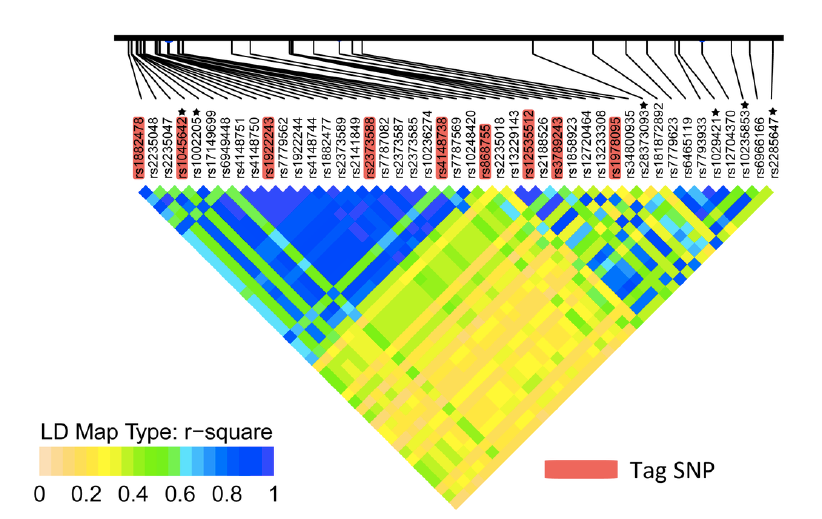
\includegraphics[width=0.95\textwidth]{LD_plot.PNG}
	\caption{Linkage disequilibrium plot.} 
	% #TODO come andrebbe letta esattamente?
	\label{fig:LD_plot}
\end{figure}


In figure \ref{fig:LD_plot}, the colors indicate the strenght of pairwise
linkage disequilibrium (LD) according to r2 metrics. Tag SNPs are shadowed in
pink. A \textbf{Tag SNP} is representative of a region with high linkage
disequilibrium and represents a group of SNPs (called haplotype).


\subsection{Other SNPs features} 
\begin{itemize}
	\item Choose SNPs that are in areas that are not likely to undergo somatic
	aberrations. So \underline{exclude chromosomal locations which undergo
	frequent somatic aberrations}. Eg. areas commonly deleted in tumor will
	produce LOH but probably also no calls, since there is no DNA. 
	\item Choose \underline{SNPs equally represented}/spread all around the
	genome (not in specific chromosome regions).
	\item Select \underline{autosomal only SNPs}.
	\item Select \underline{SNPs in exons}. If we were to run a targeted assay,
	this would cover more exons instead of intrones. It will also be more
	probable to have signal from a non-DNA assay, for example if calling a
	genotype from RNA sequencing data (even though it is not always done).
	\item Exclude/include \underline{disease or drug response associated loci}. 
	\item Include/exclude loci with significantly \underline{different MAF in
	different ethnicity}. If we include them we can also have a lineage type of
	tests in the same assay. 
\end{itemize}


\subsection{Number of SNPs to select} 

If we want to build a test to run genetic fingerprinting using SNPs, \textbf{how
many polymorphic loci (SNPs) should be tested?} We want to make sure that the
measure of the test will be able to differentiate unrelated individuals. But we
must also remember that many variables must be taken into account, possible
mismatches in particular. Those can be due to the sequencing process itself
(experimental mismatches) but also to changes due to somatic events (biological
mismatches). All these events can be used in the test with a different weight,
based on how likely they are. 


\subsubsection{Experimental mismatches : Genotype call error rate}

During sequencing, each machine will produce some errors, resulting in some loci
for which no data will be available. If those loci include some SNPs of
interest, then no call will be associated to that SNP. Experimental mismatches
are related to the error rate of the technology used, they are platform
dependent. 

\paragraph{Some examples:}

\begin{figure}[ht]
	\centering
	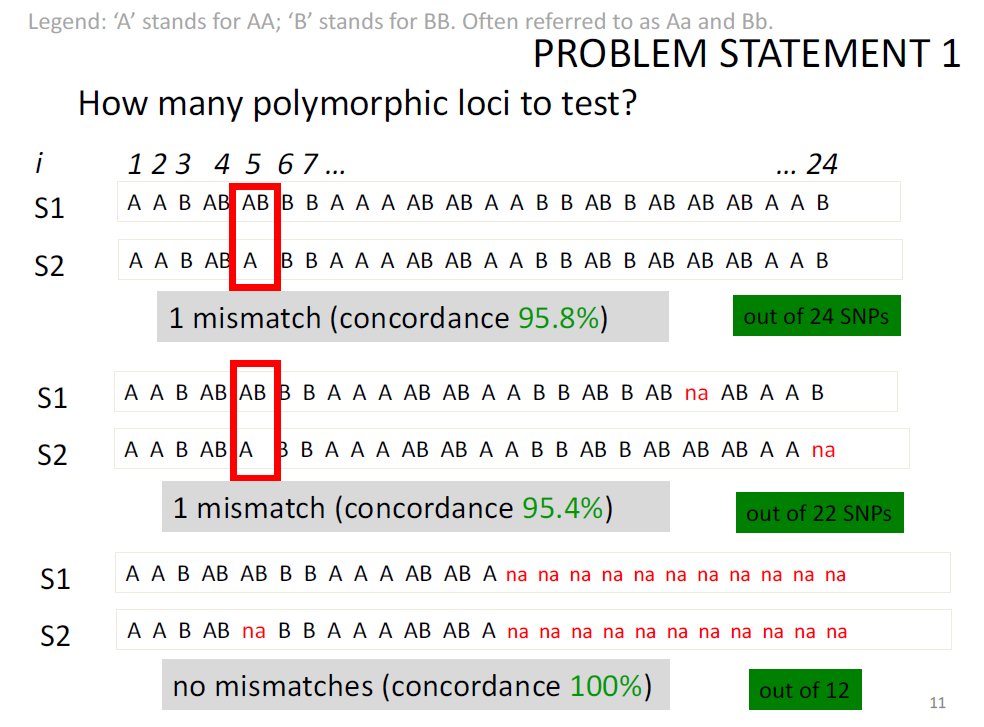
\includegraphics[width=0.7\textwidth]{SNP_number.PNG}
	\caption{'A' stands for 'AA' (e.g. homozygus genotype for the reference
	allele); often refered to as Aa. 'B' stands for 'BB' (e.g. homozygus
	genotype for the alternative allele); often refered to as Bb. 'AB' stads for
	heterozygus.}
	\label{fig:SNP_number}  
\end{figure}

In each example in figure \ref{fig:SNP_number} there are two samples with the
same number of potential SNPs: 24. To detemine the difference/similarity
(concordance) of the two samples we can look at the genotype for each position
and count mismatches.

Legend: 'A' stands for 'AA' (e.g. homozygus genotype for the reference allele);
often refered to as Aa. 'B' stands for 'BB' (e.g. homozygus genotype for the
alternative allele); often refered to as Bb. 'AB' stads for heterozygus.

\begin{itemize}
	\item \textbf{First Example}: over the 24 loci, there is only one mismatch.
	This translates to a level of concordance of 95.8\%. Those 2 individuals are
	highly related or DNA comes from the same saples. 
	   
	\item \textbf{Second example}: there is only one mismatch but there are some
	'na', indicating that for some positions we don't have a call (not available
	data). Therefore, in this case the concordance is measured out of 22 SNPs
	and is equal 95.4\%. 

	\item \textbf{Third example}: here a lot of 'na's are present, leading to
	have only 12 SNPs available. This brings to a concordance of 100\%. 
\end{itemize}

Different examples produced different levels of concordance. What do we trust
the most?

The first set of SNPs is the one that we trust the most, because it has the
higher number of available SNPs. Wider number of SNPs provides the most reliable
information. 

\subsubsection{Biological mismatches}

In the context of desease samples and tumors, many somatic events can happen,
like deletions, gains of copies, homozygus deletions, ecc. Some common ones are:
\begin{itemize}
	\item  \textbf{Loss Of Heterolzygosity (LOH)}:  event that results in loss
	one parental copy of a region which results in the genome having just one
	copy of that region. If that region contained a heterozygus locus (e.g.
	SNP), there will be loss of Heterozygosity. $AB \rightarrow A$.
	\item \textbf{Gain Of Heterozygosity (GOH)}: due to a mutation in a site
	often polimorphic through inheritance. These are pretty rare. $A \rightarrow
	AB$. 
	\item \textbf{Double Mutation (DM)}: very rare.  
\end{itemize}

\begin{figure}[ht]
	\centering
	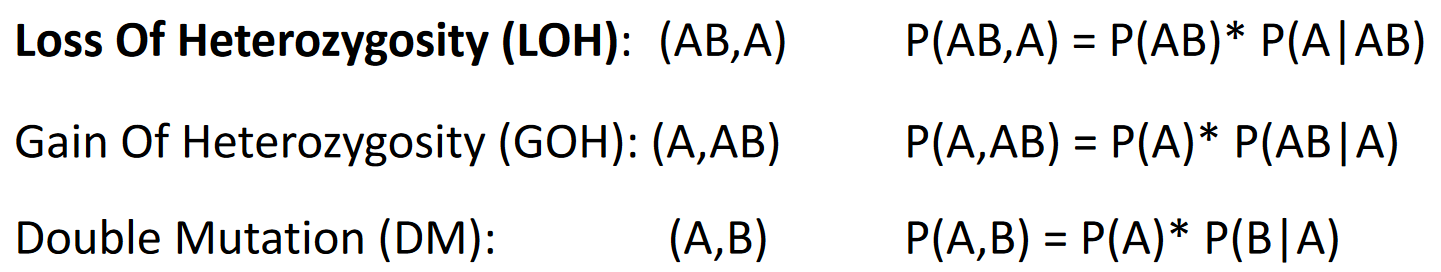
\includegraphics[width=0.75\textwidth]{heterozygosity.PNG}
	\caption{} 
	\label{fig: heterozygosity}
\end{figure}

\bigskip
Biological mismatches can be properly modeled in our assay. We can, in a data
driven way, assess the error rate for the genotyping for some specific SNPs or
run tests. We can also think in terms of SNP-specific or tissue-specific
probabilities.

The main point is that all mismatches must be taken into consideration. For
this, all implemented tests use \emph{more than the minimal number of SNPs} that
allow to identify individuals. 


\section{Genetic Distance}

Having defined the number of SNPs to use, with maximum MAF and other amanable
characteristics, the genetic test should provide a measure of some sort, which
will be the output metric, associated with a probability of the measure to be
correct. \\

As a simple measure, we can \underline{count the number of loci where two
samples show different genotype} and normalize on the total number of queried
loci, defining a certain level of discordance (or concordance). The output value
will be the '\textit{genetic distance}' between the two samples given the
selected loci. The distance is proportional to the number of discordant calls.
\\

In figure \ref{fig:Distance} we can see an example of a typical graph used to
measure the genetic distance using SNP-based genetic testing. We have 4 samples
with a set of 5 SNPs for each one. The distance is measured among all possible
pairs, whose indexes are reported on the x-axis. 

\begin{itemize}
	\item s1 and s2 have 3 A in common, one locus has no call and another one
	produces a mismatch. 1 mismatch out of 4 produce a distance of 0.25.
	\item samples s1 and s3 have 5 mismatches out of 5, so a distance (or
	discordance) of 1. 
\end{itemize}


\begin{figure}[ht]
	\centering
	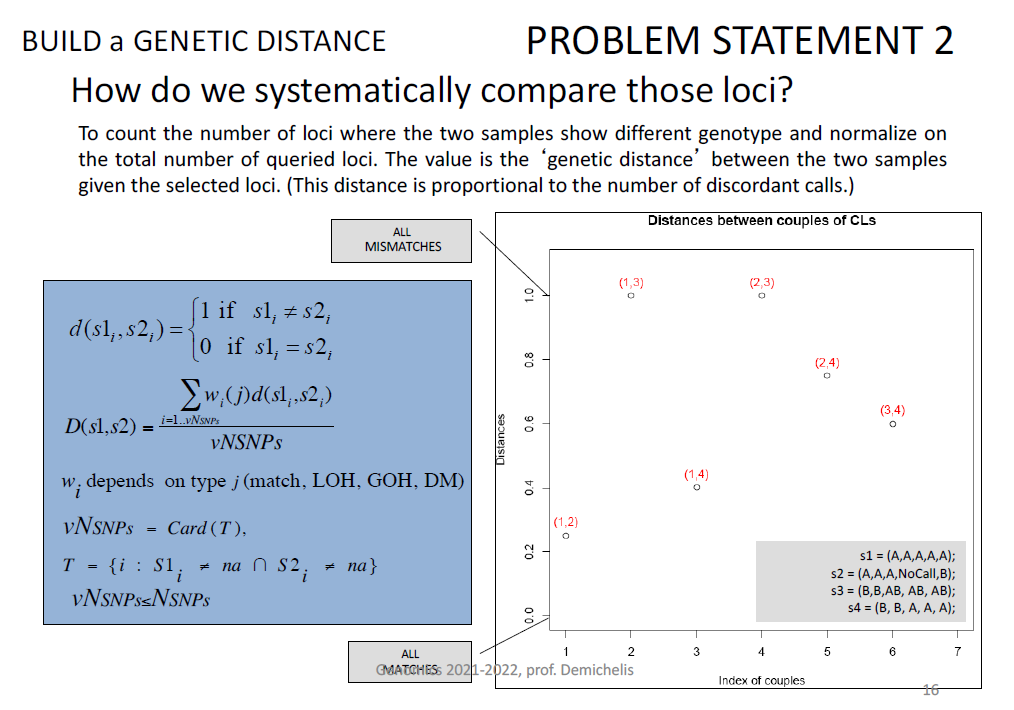
\includegraphics[width=1\textwidth]{Distance.PNG}
	\caption{Genetic Distance graph with 4 samples}
	\label{fig:Distance} %#TODO metti label sotto caption
\end{figure}

If we put that into an equation in \ref{fig:Distance} will have that: for each
position $i$ (SNP) bwteeen sample 1 and 2 we can have 1 if the genotype is
different, 0 if they are identical. Then we determine the distance D by summing
up the different scores obtained for each SNP. We can associate different
weights $w_i$ to different mismatches (depending on Gain Of Heterolzygosity,
Loss Of Heterolzygosity, Double Mutation) or we can put all equal to one. Then
we devide by the total number of SNPs for which we have available calls vNSNPs
for both the sequences in comparison, which will be lower or equal to the total
number of SNPs, NSNPs. 


\begin{figure}[ht]
	\centering
	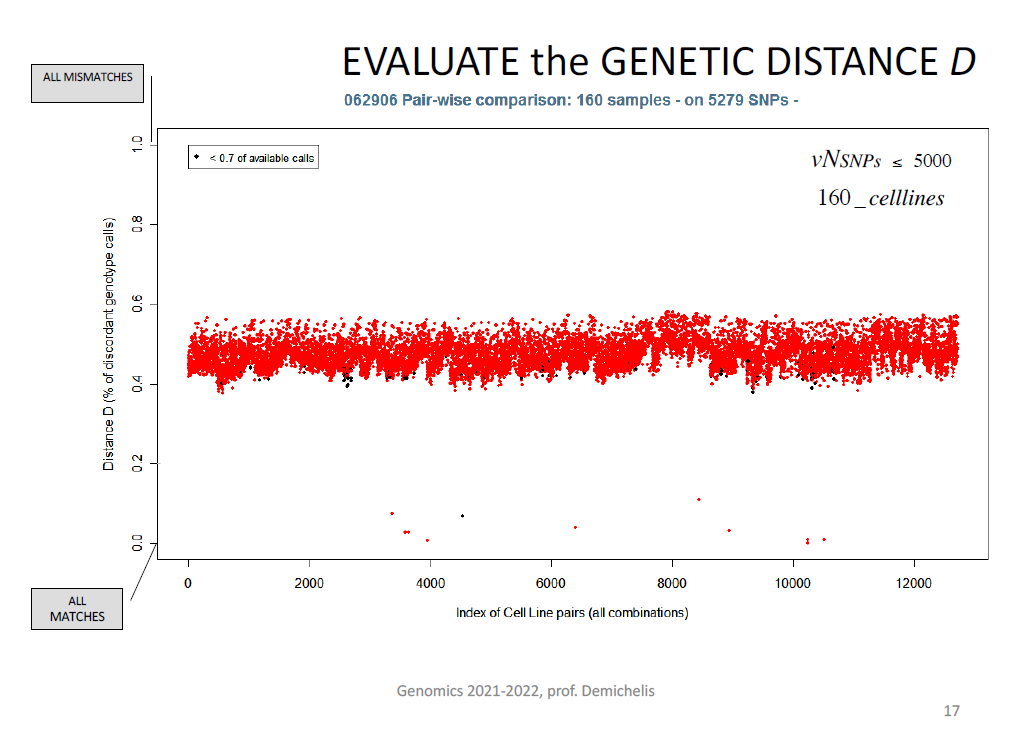
\includegraphics[width=0.9\textwidth]{Distance2.PNG}
	\caption{\label{fig:Distance2}Genetic Distance graph with 160 samples}
\end{figure}

\bigskip
This other example at figure \ref{fig:Distance2} shows the distance, measured by
genetic fingerprinting, of a collection of 160 samples of cell lines. 

The number of possible pairs corresponds to: $\frac{160 \cdot 159}{2}$ (number
found in the x-axis). 

By applying this measure to a larger collection of samples like this one, with
many SNPs, we expect to find an \textbf{average distance} among all possible
pairs that very unlikely will be close to 1. 

The MAF of the SNPs is 0.5 but it will never happen that, with a high number of
SNPs, the discordance will be 1, meaning that the SNPs will be all different. We
will have an average distance that in this case around 0.5, since by chance we
all share some genotypes on a large number of SNPs. 

Here they found certain pairs with a very low distance, sometimes almost equal
to zero (dots at the bottom). This was a surprising result because it shows that
those pairs, which were suppose to be different cell lines, were actually not
different cell lines (only less than 70\% of SNPs have available calls). 


\begin{figure}[ht]
	\centering
	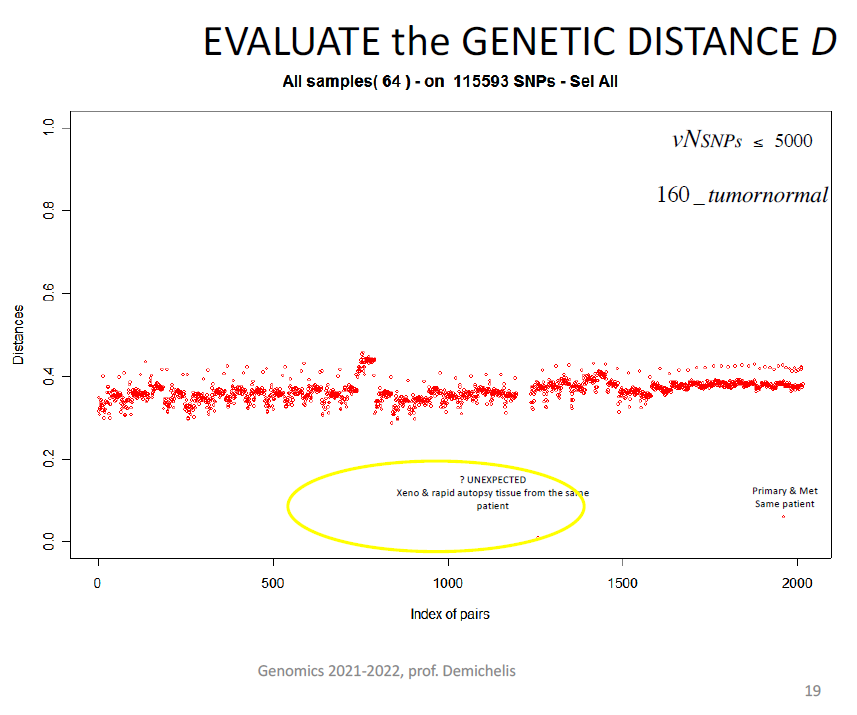
\includegraphics[width=0.9\textwidth]{Distance3.PNG}
	\caption{\label{fig:Distance3}Genetic Distance graph with tumor samples}
\end{figure}

\bigskip
In this last example at figure \ref{fig:Distance3} genetic fingerprint was
performed on a collection of 160  tumor samples, with a larger SNP array (more
that 100.000 SNPs).  

From the analysis, two samples with very low distance were observed. One of the
two samples came from a Rapid Autopsy Progam and the other one from a xenograft
model. 

\underline{RAP} are programs for which patients at the end of their life agree
to donate their tumor tissues which can be used for research. In these very
complex but highly valuable programs, the material must be taken within two
hours after death. Those samples are usually higly caractherized but after a
while the track of the patient's identity is lost. Here, what happened is that
one man who donated tissue to this program was sequenced and for some of those
metastasis models were generated and implanted into a mouse and a xenograft
model was derived. Thanks to fingerprinting it was possible to determine the
same origin between xenograft and patient. 

The power of this tecnique is very high, it allows also to identify and remove
things that we don't want in our study. Eg. if running a study (like a GWAS
study) on a certain \underline{interesting geopraphic area}, we will want to
remove the members of the same family because that would skew the results.
Genetic fingerprint can be used for this purpose.

\subsection{Some questions}

\noindent\textbf{Q1}: \textbf{\textit{Would the average of unrelated samples
distance increase or decrease after selection of ideal SNPs?}}\\

If we use SNPs likely to be different among individuals and we use them to
determine the measure of the ditance, then the average value of unrelated
individuals will increase.\\

\noindent\textbf{Q2}: \textbf{\textit{Is it likely to obtain a genotype distance
D = 1?}}\\

We get distance 1 only if we are looking at too few viable SNPs. Whereas with a
well selected pool of SNPs, and a high enough number of SNPs, it is very
unlikely that the distance is equal to 1.

\subsection{Further considerations}
How does the genetic distance among different samples change when varying the
number of selected SNPs used to perform the test?

\begin{figure}[ht]
	\centering
	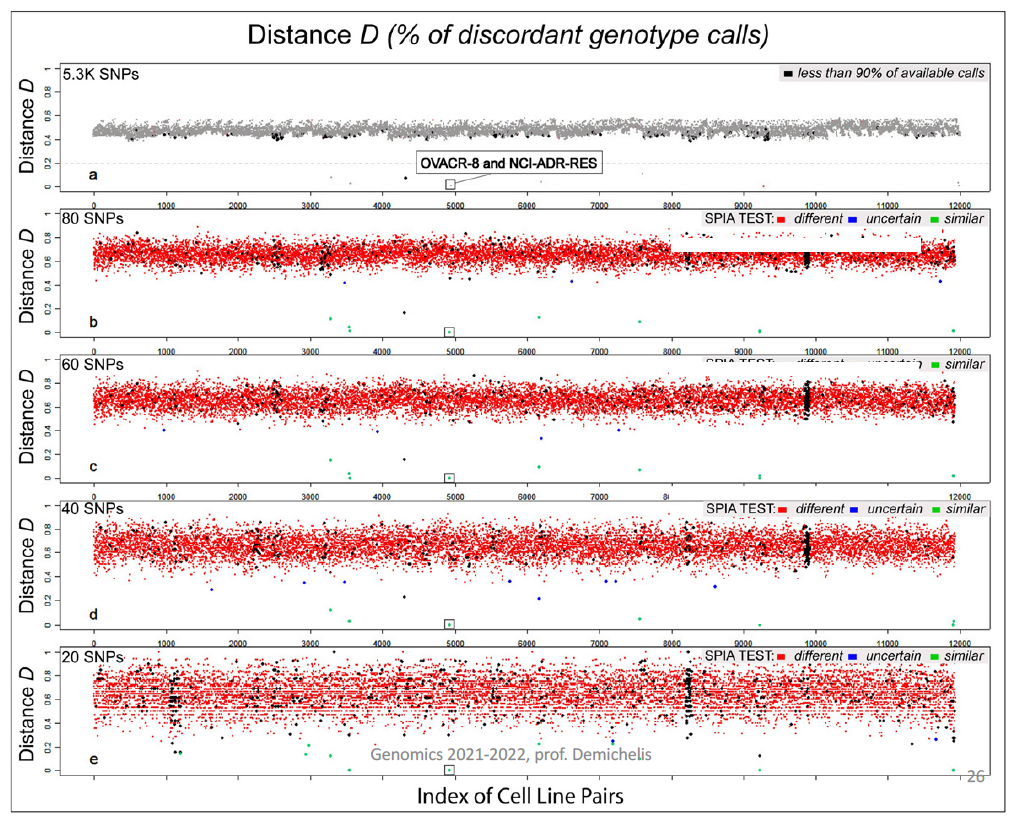
\includegraphics[width=1\textwidth]{Selected_SNP.PNG}
	\caption{Genetic Distance graph at deacreasing number of selected SNPs}
	\label{fig:sel_snp}
\end{figure}

The genetic distance among many samples, with an array of 5.3K SNPs, was
measured, using a decreasing number of SNPs (from the initial total number of
SNPs to decreasing numbers of highly selected SNPs) \ref{fig:sel_snp}. \\

It is noticeable that, in the second plot where 80 SNPs matching the required
characteristics were selected, the average Distance across all pairs is higher
than in the previous example, in which all available SNPs were used ($\sim 0.45$
vs. $\sim 0.65$). Also, the standard deviation of greater. Decreasing the number
of SNPs to 60, then to 40 and 20 leads to have the same average distance between
pairs, which settles around 0.66, but higher standard deviation.

In reality we always need enough SNPs, enough information, in order to prevent
unexpected issues and to be sure that for any pairs of sample we have enough
information to trust our measure. 


\section{Building a SNP-based genetic test}

Building an identity test base on SNPs is a MULTI-STEP process, consisting in: 
\begin{enumerate}
	\item Definition of a genotype/genetic distance to compare samples;
	\item Definition of SNPs requirments, based on the intention of the assay.
	\item Selection of SNPs:
	\begin{itemize}
		\item This can be done in a data-driven manner, through an iterative
		procedure of training and test on known sample set;
		\item Or, performing the selection based upon MAF and Hardy-Weinberg
		equilibrium. For example, using HapMap data.
	\end{itemize}
	\item Implementation of a probabilistic test (different, uncertain or
	similar)
	\item In silico validation on independent/multiple dataset.
	\item Validation on cell lines genotyped on independent platform. 
\end{enumerate}
We have already seen some of the steps needed (1, 2, 3), we now pass to the
following ones.


\subsection{Implementation of a probabilistic test} 

Other important questions which we have to answer to when designing a genetic
test are:
\begin{itemize}
	\item What is the \textit{threshold} on the genotype distance to call two
	samples 'identical' ('similar') or 'different'?
	\item How \textit{confident} would the call be?
    \item What is the \textit{minimum number} of loci needed for a robust test?
\end{itemize}

It could be useful to have a probabilistic test to determine if the measure of
the test is correct at which level of confidence. We can use a probabilistic
approach to compare observations with expectations (gold standard).

\bigskip
Under the assumption that SNP calls at different loci are independent, we can
think in terms of Binomial distribution. Each SNP can be considered as a trial,

\begin{itemize}
	\item $n$ = number of SNPs in the assay, 
	\item $k$ = number of matches, 
	\item $p$ is the probability of match and ($1-p$) of mismatch.
\end{itemize}

Then the probability of having k matches (successes) out of N SNPs (trials)
follows the binomial distribution. With $n$, $np$ and $np(1-p)$ large enough, we
can use the \textbf{Gaussian approximation} of the Binomial distribution with
$K_{\text{mean}} = np$ and $sd = \sqrt{np(1-p)}$. \\


\begin{figure}[ht]
	\centering
	\begin{subfigure}[t]{0.80\textwidth}
		\centering
		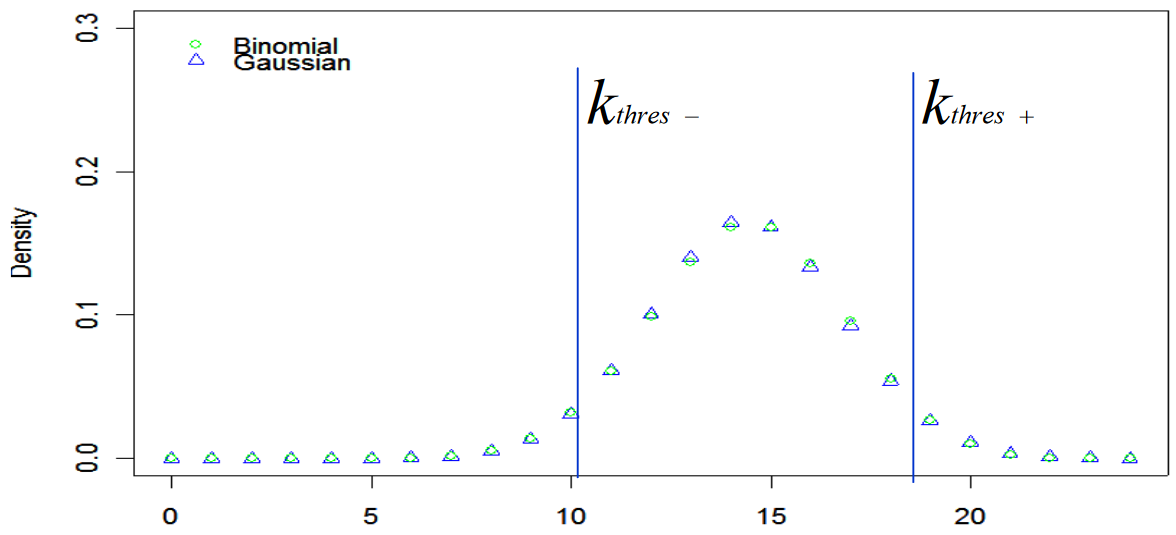
\includegraphics[width=1\textwidth]{binomialDistSNPsmatches.PNG}
		\caption{The probability binomial distribution could be approximated to a Gaussian when the number of cases is large}
		% \label{subfig: }
	\end{subfigure}
	\hfill
	\begin{subfigure}[t]{0.80\textwidth}
		\centering
		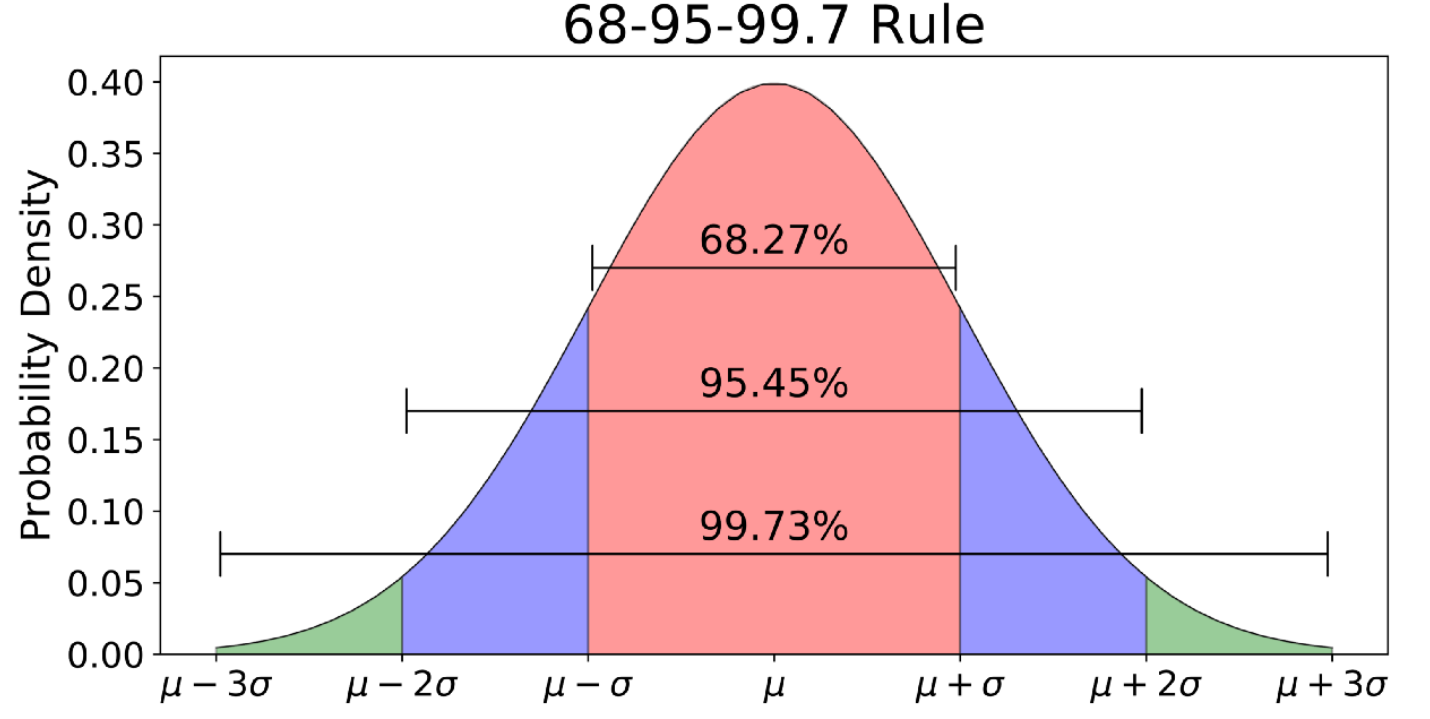
\includegraphics[width=1\textwidth]{gaussianity-binomialdist.PNG}
		\caption{Percentages Gaussian distribution}
		% \label{subfig: }
	\end{subfigure}
	\caption{Approximation of a binomial distribution to a Gaussian and
	percentages related.}
	\label{fig: binomial distribution SNP matches}
\end{figure}

With something that simple we can add a probabilistic test in our assay,
defining an area of confidence given by $K_{\text{mean}} \pm m \cdot sd$ where m
is the number of standard deviations used to define the thresholds which will
lead to have a smaller or wider confidence area. 

%immagine slide 33
\begin{figure}[ht]
	\centering
	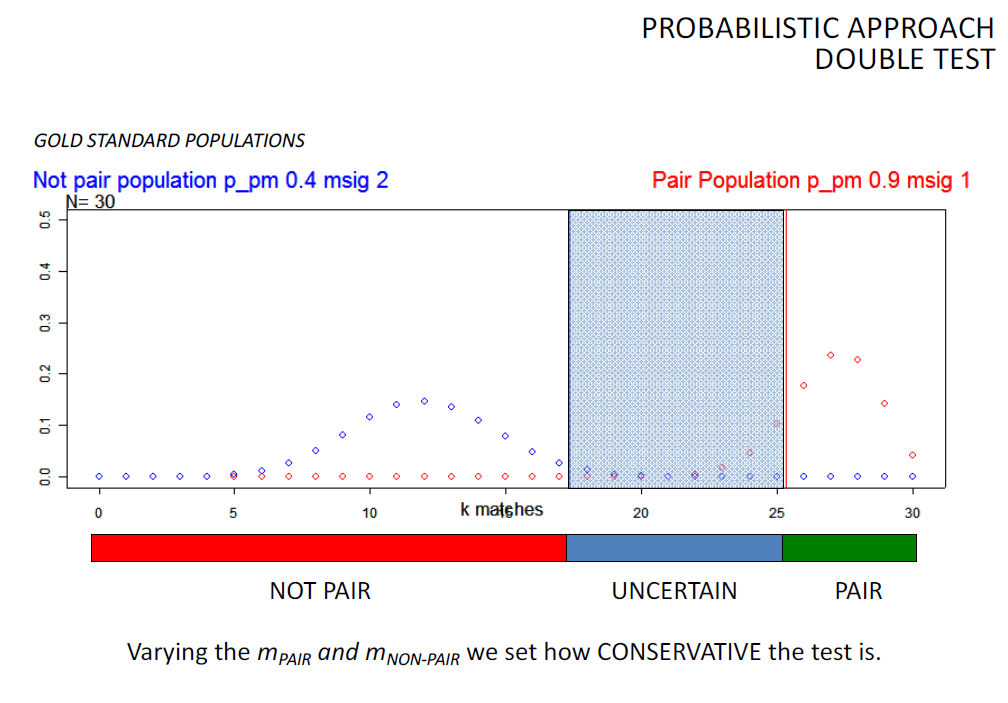
\includegraphics[width=0.9\textwidth]{Prob_test.PNG}
	\caption{\label{fig:prob_test}}
	% #TODO not pair populations? paired populations? Don't understand the
	% meaning of these things
\end{figure}


\bigskip
So for example: given two unrelated samples, we reason in terms of  
'\textit{what is the probability of having a certain number $k$ of matches over
a total number of n SNPs, therefore a certain value of D?}'.\\
\noindent The probability mass function for unrelated individuals is shown in
figure \ref{fig:prob_test} with a blue dotted line and indicates that there is a
low probability of having both a very low and a very high number of matches (it
is assumed that the comparisons of samples follow a binomial distribution, where
higher and lower values, compared to the mean, have less likely). 

\noindent We can also think in the opposite term: given two related samples,
what is the probability of having  matches? As represented by the red dotted
line, in this case there will be a high probability of having many matches. 

Using these probabilities we can set two thresholds which will define 3 regions:
\begin{itemize}
	\item A \textbf{'not pair'} region for which the two samples will be
	considered as 'different'.
 	\item a \textbf{'pair'} region for which the two samples will be considered
 	as 'similar'.
	\item and an \textbf{'uncertain'} region, a grey zone, for which no certain
	result can be produced. 
\end{itemize}

Then we can move the grey area based on what we want to be certain of and on how
many SNPs we have.

By decreasing the number of SNPs, the grey zone will become more tiny, making
the result more difficult to interpret. For example, a difference of only 2
matches could lead to opposite conclusions. 

By contrast, with more SNPs the area will be wider and easier to interpret.
Hence using a number of SNPs greater than the minimum number is better,
otherwise there will be many uncertain calls. 


\section{Further considerations and examples}
%sistemare
In the past, before sequencing area and SNPs array area, \underline{short tandem
repeats} were commonly used for genetic fingerprint. They were used on gels to
distinguish related and unrelated individuals, eg, for the initial paternity
test.\textbf{ Di-nucleotide markers} are the most informative class of
microsatellites. Generally they are more informative than SNPs, though selected
SNPs perform quite well.\\

\textbf{Inherited copy number variants} can be used too for a fingerprinting
test, but not all of them. The more amenable for this test are the loss type of
CNV. In the population there will either a copy number of 2 or 1 or 0. If both
parents have heterozygus pair of CNVs it will be possible that I have a
homozygus deletion. If both parents have 2 copies at a site that is polimorphic
in the population, we will have a genotype equal to 2 copies. \\

If we think about \textbf{gain} of CNV then it becomes messy, because when
combining multiple copies and have a add up we cannot distinguish what comes
from what pair, so we cannot use them to identify an individual.


\subsection{Example 1: Cell line passages}

A mass use of these genetic tests is done to assess \textbf{genetic changes in
in-vitro cultivation}. Cell lines go through multiple passages in which they are
used and stored. Genetic fingerprinting can be used to assess if among different
passages the cells have remained the same, if they were mislabeled or if major
genetic drifts happened. Genetic fingerptinting is also used in studies of tumor
evolution, lineage plasticity, etherogenity across metastasis across individuals
or a single tumor. 

% #TODO add to definitions
\textit{Lineage plasticity}, the ability of cells to transition from one
committed developmental pathway to another, has been proposed as a source of
intratumoural heterogeneity and of tumour adaptation to an adverse tumour
microenvironment including exposure to targeted anticancer treatments.

In this example (figure \ref{fig: cell lines comparison}), two types of prostate cell lines
which underwent multiple passagges were used: \textit{\textbf{N15C6}} (passages
from 48 to 63) and \textit{\textbf{N33B2}} (passages from 21 to 39). The cell
lines were profiled with a SNPs array and the assay was run. All passages of
each cell lines were compared with all other passages. We expect all passages to
have the same genetic fingerprinting in the same cell line.\\ 

However the results obtained using the \textbf{full array of SNPs (50k)}
(subfigure \ref{subfig: 50k SNPs}), showed that some pairs which should be
exactly identical (distance equal to zero) are actually a bit different 
% #TODO shouldn't it be correct?
(points at the bottom-left). By contrast, by using a set on only 54 SNPs
(subfigure \ref{subfig: 54 SNPs}), this diversity is not detectable, indicating
that using the restricted number of SNPs could make us loose some information. 

% #TODO ???
\begin{figure}[ht]
	\centering
	\begin{subfigure}[t]{0.80\textwidth}
		\centering
		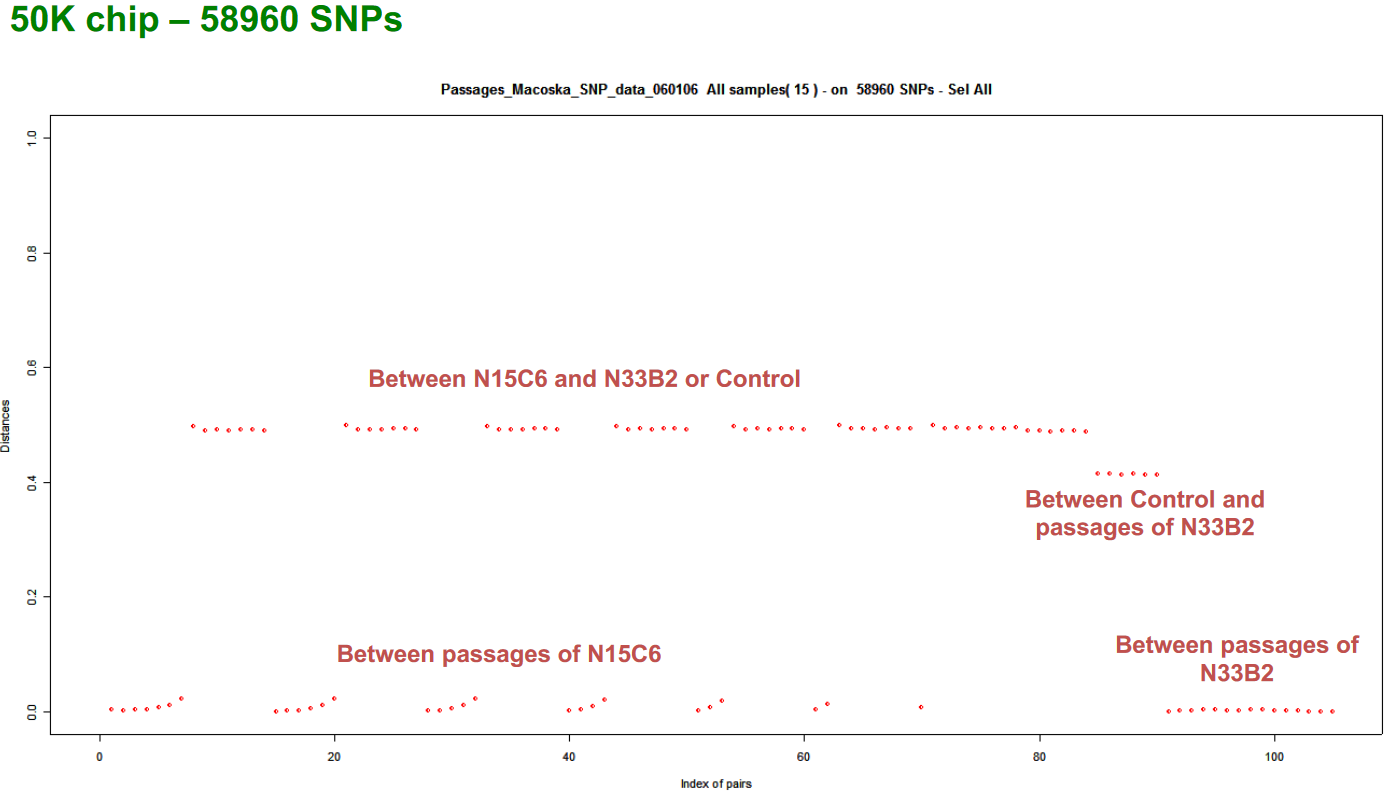
\includegraphics[width=1\textwidth]{50Kchip.PNG}
		\caption{Comparing passages with the total amount of available SNPs}
		\label{subfig: 50k SNPs}
	\end{subfigure}
	\hfill
	\begin{subfigure}[t]{0.80\textwidth}
		\centering
		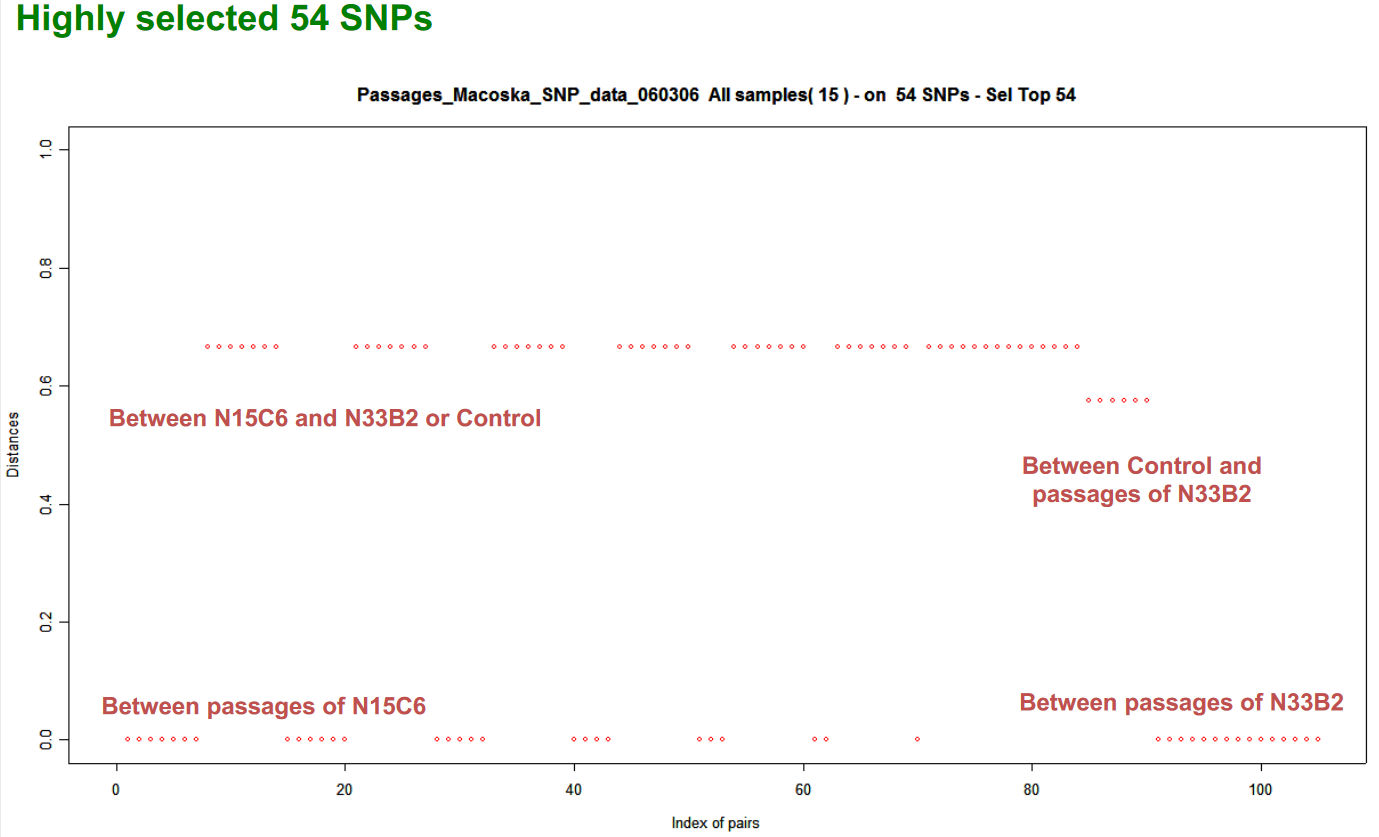
\includegraphics[width=1\textwidth]{54SNPchip.PNG}
		\caption{Comparing passages with 54 SNPs}
		\label{subfig: 54 SNPs}
	\end{subfigure}
	\caption{}
	\label{fig: cell lines comparison}
\end{figure}


In order to understand this increase of distance, they looked at each chromosome
to see if there were problems that justified increase the increased distance
expected to be equal to zero in that cell line. All chromosome were tried. If we
focus only on the SNPs spread across Chromosome 11, we observe that there is a
major difference for certain passages with respect to the initial ones, only for
one cell line (N15C6). This was due to the way the cells were immortalized
(insertion in chromosome 11), look to figure \ref{fig: chr 11 SNPs}.

\begin{figure}[ht]
	\caption{Comparison passages regarding chr 11}
	\centering
	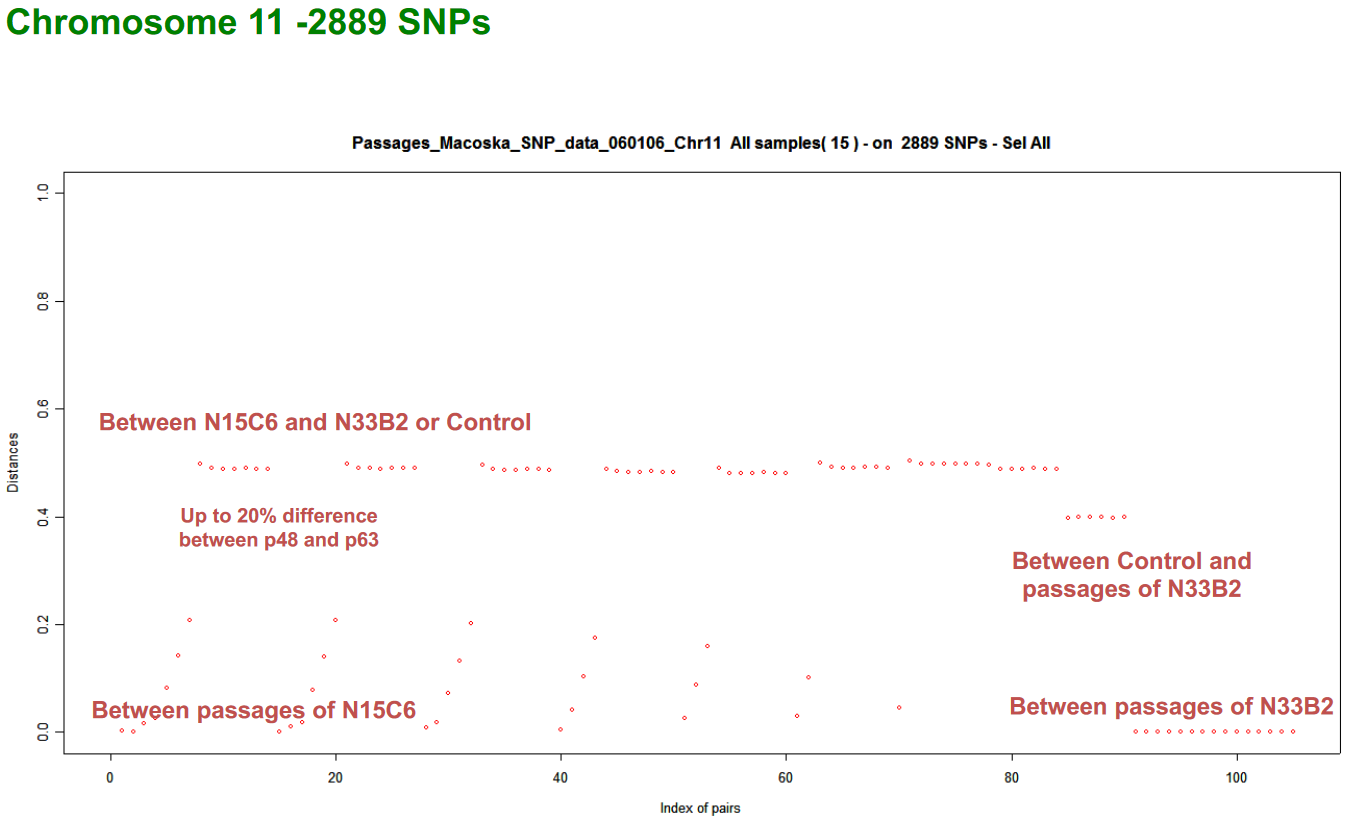
\includegraphics[width=0.8\textwidth]{chr11chip.PNG}
	\label{fig: chr 11 SNPs}
  \end{figure}


\subsection{Individual's Relatedness (genotype-distance)}

The HapMap consortium sequenced hundreds of individuals for different
ethnicities and also used trios. \textbf{Trio sequencing} is a technique which
involves the sequencing of the genome of \underline{mother, father and
son/daughter}. Trios provide major information for haplotype blocks, for
identifying regions related to inheritance, ecc.

% immagine slide 43
\begin{figure}[ht]
	\centering
	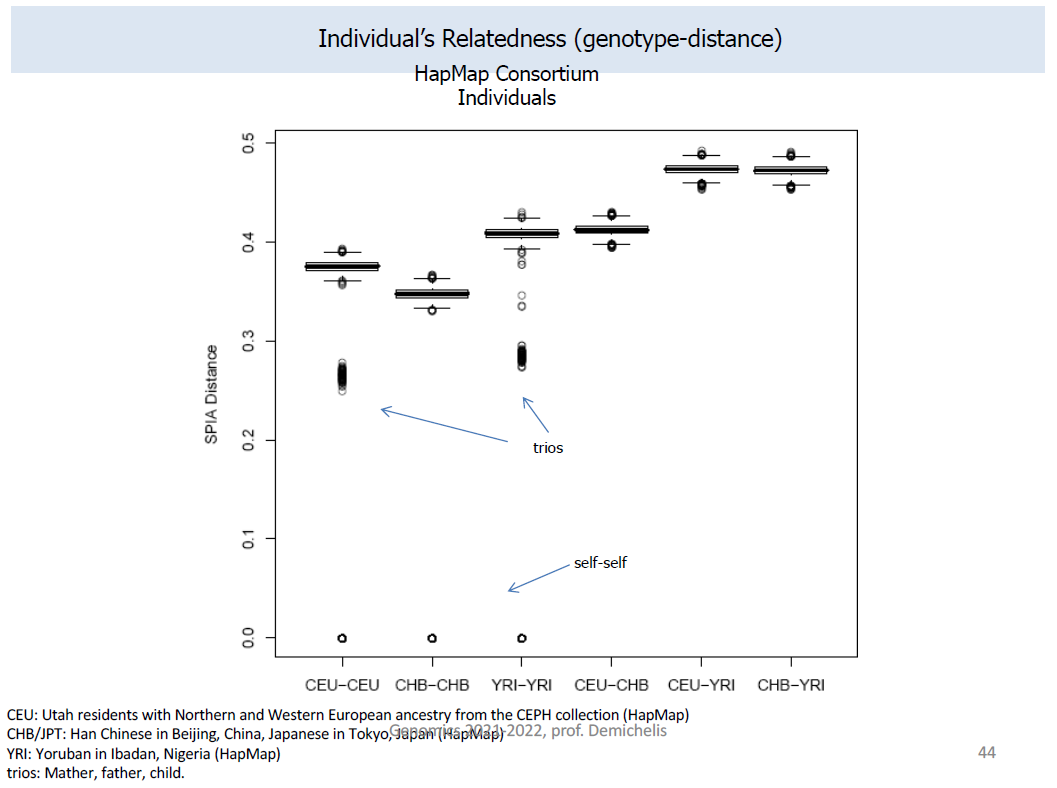
\includegraphics[width = 1\textwidth]{trios.PNG}
	\caption{\label{fig: trios}}
\end{figure}

By looking at the data based on \textit{SPIA Assay} (subsection \ref{subsect:
SPIA}) (a genotype base assay which measures distance) at figure \ref{fig:
trios} we see that self-self pairs have distance zero, as expected; samples
within each ethnicity have a certain average distance, which is lower than the
distance observed among different ethnicities. Differences in distance among
mixed samples are due to the fact that the SNPs used had on average higher MAF
in some populations than in others. \\
\noindent We also notice that in trios the distance is not 0 and is not equal to
the median distance of unrelated individuals. This can be used for paternity
tests or even in forensic science (figure \ref*{fig: Relatedness of
individuals}).

\begin{figure}[ht]
  \caption{Relatedness between individuals can be evaluated through SNPs}
  \centering
  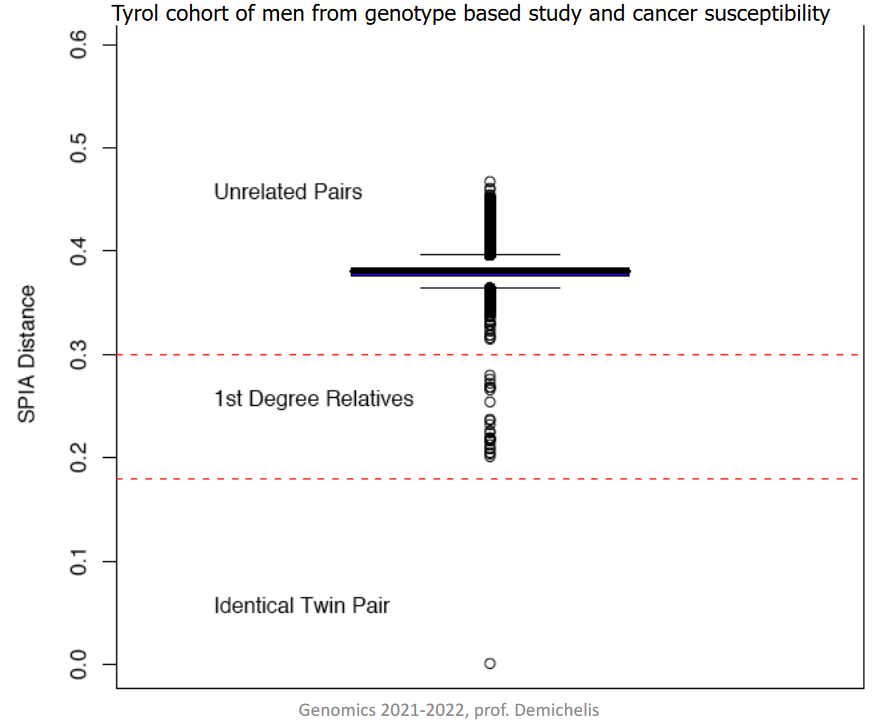
\includegraphics[width=0.60\textwidth]{IndividualsRelatedness.PNG}
  \label{fig: Relatedness of individuals}
\end{figure}

% #TODO have to clarify figure page 42

\subsection{Example 3: Cancer supscettibility test}
% #TODO to which data are you referring?
The data showed refers to a study were they were looking for polimorphisms that
increase the \textbf{likelihood of prostate cancer}. In these studies, if
relatives are present in the cohort, only one of them is taken to avoid skewing
the results. When looking for signs of cancer susceptibility by performing
genetic fingerprinting, the division based on the degree of relativeness was
determined 'for free' and could be used to remove unwanted samples from the
cohort.


\subsection{Genetic structure of the human population}

Undestanding the genetic structure of human populations is of fundamental
interest to medial, forensic and anthropological sceinces. 

The goal of association studies is to \underline{\textbf{identify DNA variants}
that affect disease risk} or other \underline{traits of interest}. However,
association studies can be confounded by differences in ancestry. \\
	
\textbf{Misleading results} could arise if individuals selected as disease cases
have different ancestry, on average, than healthy controls. The differences in
the markers wouldn't be due to the disease itself at this point, instead it
would be caused by the different origin. If in a study all controls are of the
same ethnicity and the test is done on an individual of a different ethnicity
than the test is biased. If we run a GWAS study using two ethnicities and we
want to uset the same markers of susceptibility worldwide, it won't work. \\

Especially in medicine and in the study of human evolution it is important to
\textbf{track the genetic background of individuals} that are involved in
studies in order to understand if the individuals are form a homogeneous
population or from genetically distant ones. More and more, clinical studies
must have declarations of the checks and interpretation of the data of the
genetic background of the individuals present in the study. It is very important
to come to results for which we know exactly what is the applicability. To avoid
spurious results, \underline{association studies often restrict their focus to a
single continental group}.\\

Advances in high-throughput genotyping technology have improved the
understanding of global patterns of human genetic variation and suggest the
potential to use large sample sets to \textbf{uncover variation among closely
spaced populations}. One important piece of information to consider when
developing methods to understand the genetic structure of a population, is to
think in term of variance, which is also relevant for human diseases. Many SNPs
have different \underline{MAFs} in different populations. If we use those, and
are able to have all of them in a simple computational way, we could be able to
infer what is one individual's genetic background in terms of origins (e.g.
chinese origins).\\

The easiest mathematical approach to assess how well SNPs can distinguish
ethnicity is by using \textbf{Principal Component Analysis (PCA)}. By running a
very simple PCA on a set of SNPs including SNPs with different MAF in different
populations we can, in a space, distinguish different ethnical groups. And we
could also start thinking at individuals' origins.\\

\emph{How accuratley can one predict an individuals geographic-ethnical
background based upon his/her geentic barcode?}

% study seen in the slides
\subsubsection{Example paper: 'Genes mirror geography within Europe'}

In the \href{https://www.ncbi.nlm.nih.gov/pmc/articles/PMC2735096/}{study seen
during lectures} they used a 500.000 (500k) single nucleotide polymorphism
array. Information about the country of origin of grandparents, parents and
other relatives was used to determine the geographical location that best
represents each individual ancestry. They run a combined study where they used a
supervised search to find the best SNPs to make inference and then they tested
it on another set of individuals. By using high confidence data (individuals
with high confidence origin data) and by using the genotypes of highly
informative SNPs for specific region-related inheritance, they were able to
\textbf{rebuild the map of some of the countries in Europe}
\ref{fig:PCA_countries}. \\

% immagine paper 
\begin{figure}[ht]
	\centering
	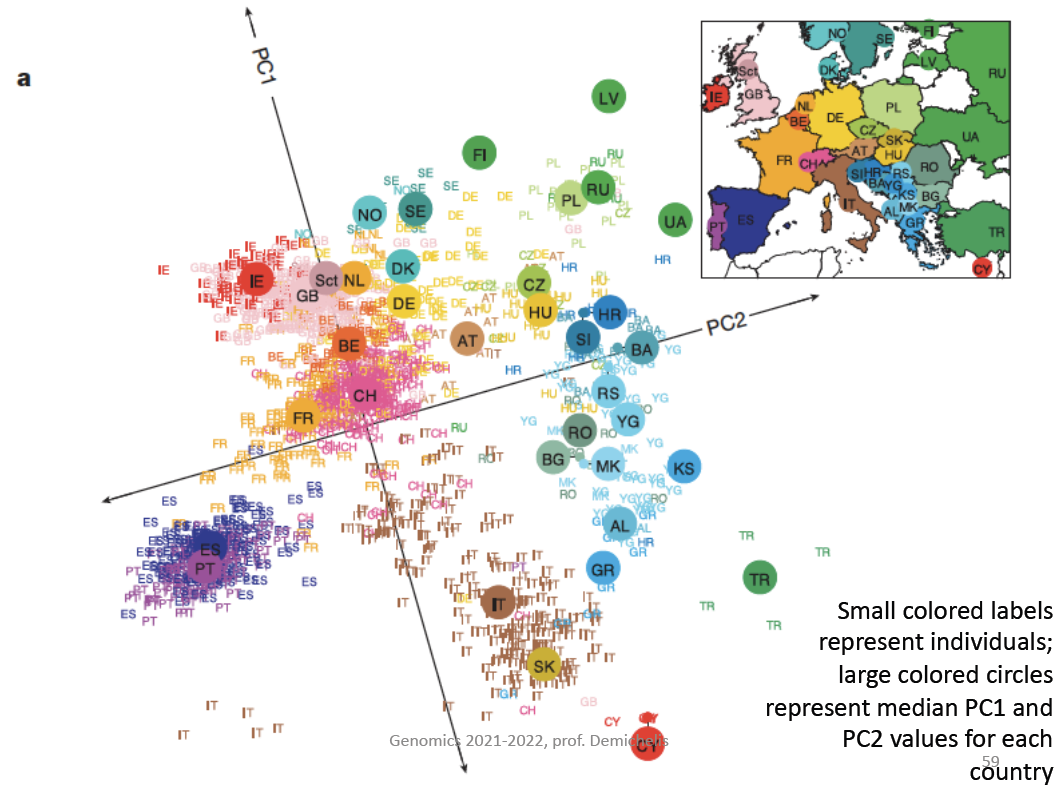
\includegraphics[width=1\textwidth]{PCA.PNG}
	\caption{Distinction of European regions thanks to SNPs.}
	\label{fig:PCA_countries}
\end{figure}

It is true that by using properly selected variants it is possible to
distinguish \textbf{individuals coming from different countries}. The way those
SNPs are selected is very similar to the process saw for genetic fingerprint,
but pushing for the selection of variants that are different in terms of MAF in
different populations. 

Clusters that are a bit more dense and distant from the others (like the
Spain/Portugal cluster) could be due to the fact that many SNPs selected are
typical of that area and are therefore able to maximize the difference between
that area and the others (so it is a data-related 'issue').
% 
% immagine 
\begin{figure}[ht]
	\centering
	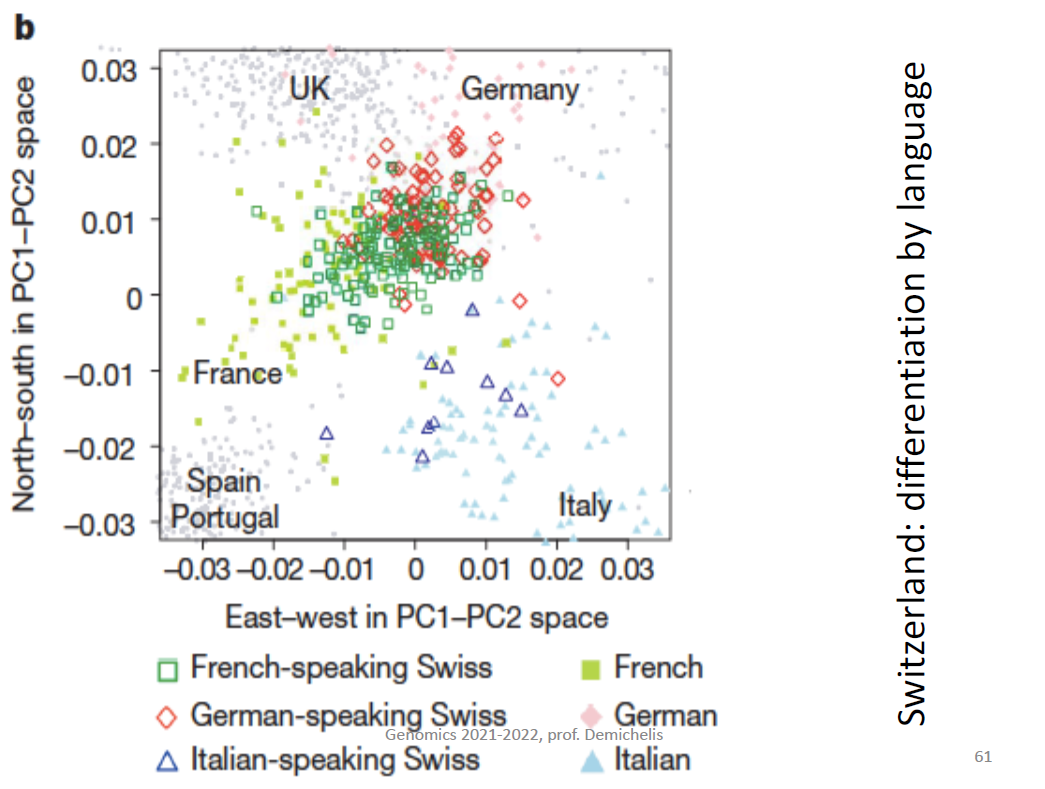
\includegraphics[width=0.8\textwidth]{PCA_swiss.PNG}
	\caption{\label{fig: PCA_swiss}}
\end{figure}

Focusing on Switzerland, they could even make inference on the linguistic canton
\ref{fig: PCA_swiss}. It is possibly true that in country where some regions
have very different cultures (e.g. marriage within the same area) might be
different between each other. 


\subsubsection{Summary and notes}
\textbf{Low-frequency alleles} tend to be the result of a recent mutation and
are expected to geographically cluster around the location at which the mutation
first arose. Hence, they can be highly informative about the \textbf{fine-scale}
population structure.

Despite low average levels of genetic differentiation among Europeans, close
correspondence between genetic and geographic distances was found. When mapping
the genetic basis of a disease phenotype, spurious associations can arise if
genetic structure is not properly accounted for.



\subsection{SPIA Assay} \label{subsect: SPIA} In a hand on lesson we performed
ourselves a SNP-based genetic distance test using the R package 'SPIAssay'. You
can find an R Markdown of that lesson in the folder 'Additional material'. 
\graphicspath{{chapters/IGVimages/}}

\chapter{IGV (Integrative Genomics Viewer)} \label{chap: IGV}

\section{Main characteristics}
The human genome nowadays is being explored extensively thanks to of exons and
whole-genome sequencing, epigenetic surveys, expression profiling of coding and
noncoding RNAs, single nucleotide polymorphism (SNP) and copy number profiling,
and functional assays. Those findings are essential to pave the way for the
future \textbf{precision medicine}. This is an approach for desease treatment and
prevention that takes into account individual variability in genes, environment,
and lifestyle for each person. The right drug, at the right time and at the
right dose for each individual. 

\begin{figure}[H]
    \caption{All the important usages of IGV}
    \centering
    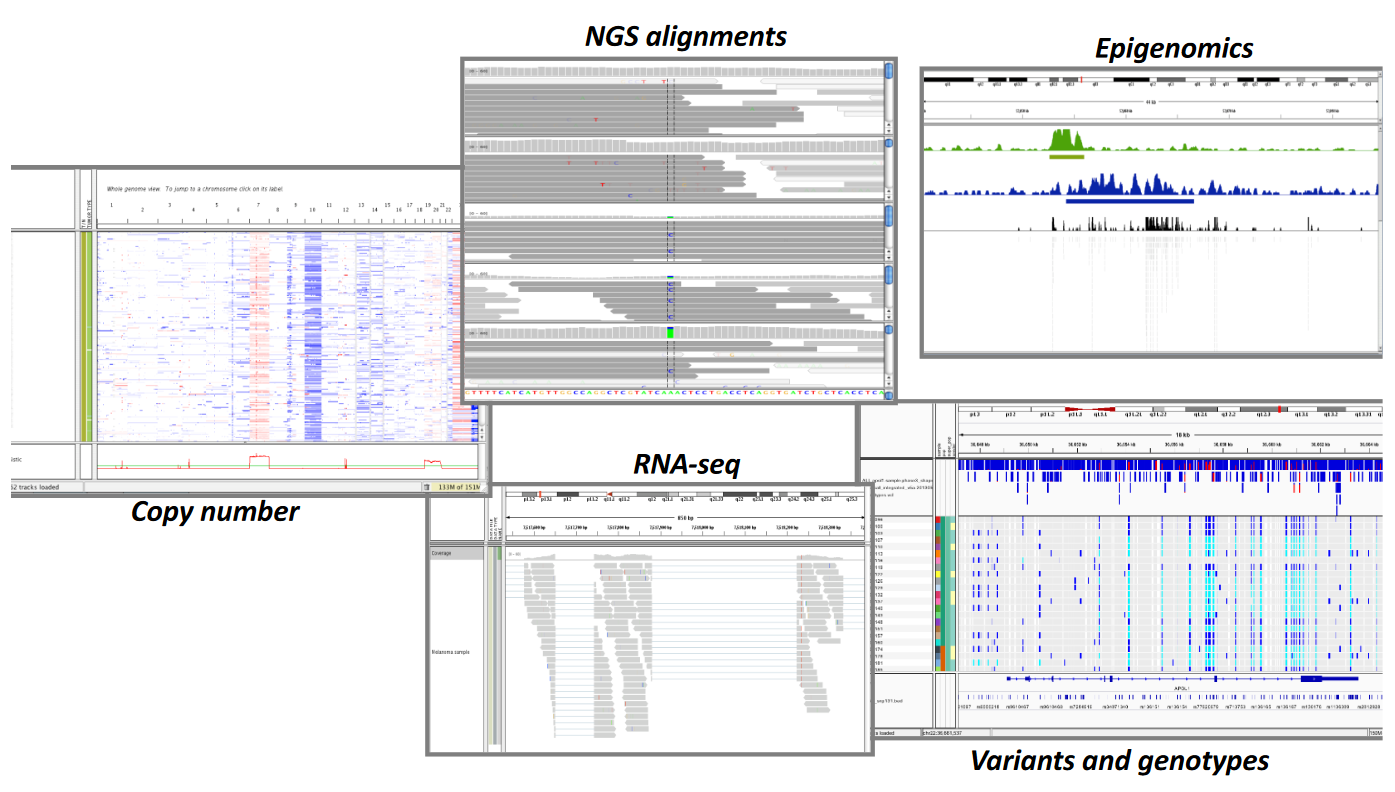
\includegraphics[width=0.6\textwidth]{usagesIGV.PNG}
    \label{IGVusages}
\end{figure}

The IGV software is an \textbf{high-performance lightweight visualization tool}
for interactive exploration of large, integrated genomic datasets. It supports a
\underline{wide variety of data types}, including next-generation sequence data,
and genomic annotations. Data sets can be loaded from local or remote sources,
including cloud-based resources. \\
It allows to move, zoom in and out quickly over different genomic scales, and also to
jump in precise positions of the sequence. It is possible to search for genomic coordinates or gene names. Pixel
resolution errors, occuring when data density exceeds the constraint given by
the number of pixels available for display, could be solved through data
aggregation. As the user zooms below the ~50 kb range, individual aligned reads
become visible. It is possible then to zoom further, and see the bases at each
position.
 
Annotations for specific genomes could be found consulting the UCSC Table Browser \href{http://genome.ucsc.edu/cgi-bin/hgTables}{(UCSC table)}.

Other information are present in the
\href{https://authors.library.caltech.edu/72234/2/nbt.1754-S1.pdf}{Supplementaty
information - Integrative Genomics Viewer} pdf file.

%#TODO For each resolution scale (“zoom level”), the aggregated data is divided into
%tiles that correspond to a region viewable on a typical user display. Each tile
%is subdivided into bins, with the width of a bin chosen to correspond to the
%width represented by a pixel at that resolution scale. During the
%pre-computation step, data in each bin is aggregated into one or more summary
%statistics as specified by the user. Data Format: the corresponding data tiles
%for each zoom level are stored in the binary Tiled Data Format, or TDF, which
%has been optimized for fast tile retrieval. - tile sizes for each zoom level
%are constant and small, - only the data needed to render the view at the
%resolution supported by the screen display. - a single tile at the lowest
%resolution (spanning the entire genome) has the same memory footprint as a tile
%at the very high zoom levels (might span only a few kilobases). Tiles no longer
%in view are discarded as needed to free memory. Navigation through a data set
%is similar to that of Google Maps, allowing the user to zoom and pan seamlessly
%across the genome at any level of detail from whole genome to base pair.

\begin{figure}[H]
    \caption{All the important elements to navigate into IGV are reported in the figure}
    \centering
    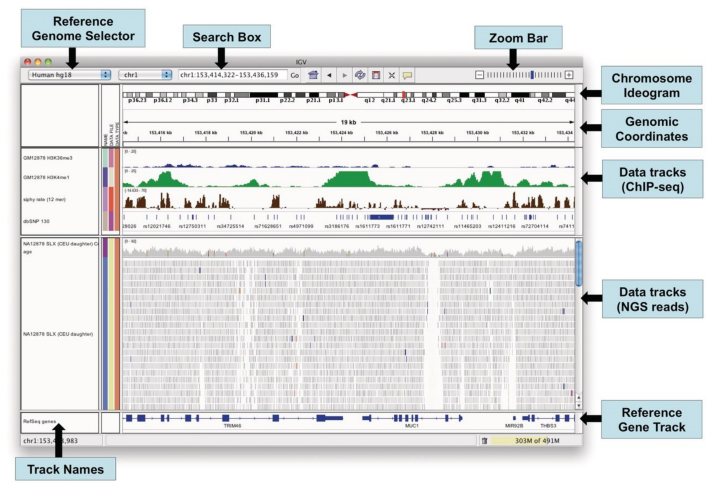
\includegraphics[width=0.7\textwidth]{IGVview.PNG}
    \label{IGVnavigation}
\end{figure}
\begin{figure}[H]
    \caption{}
    \centering
    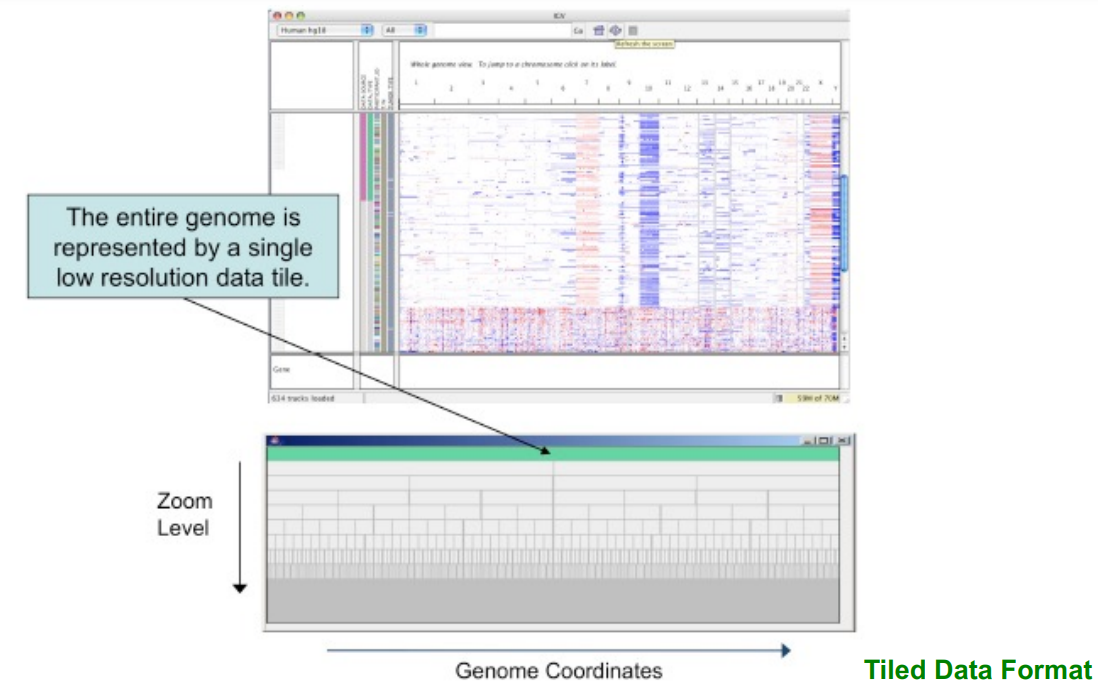
\includegraphics[width=0.6\textwidth]{Tiles.PNG}
    \label{Til}
\end{figure}
\begin{figure}[H]
    \caption{}
    \centering
    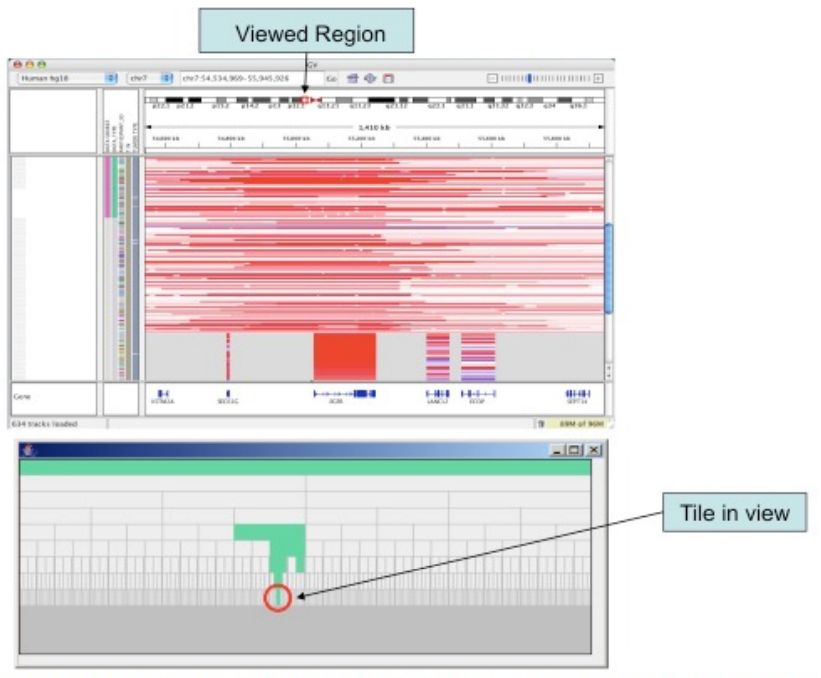
\includegraphics[width=0.6\textwidth]{TileView.PNG}
    \label{img: TileV}
\end{figure}
\begin{figure}[H]
    \caption{}
    \centering
    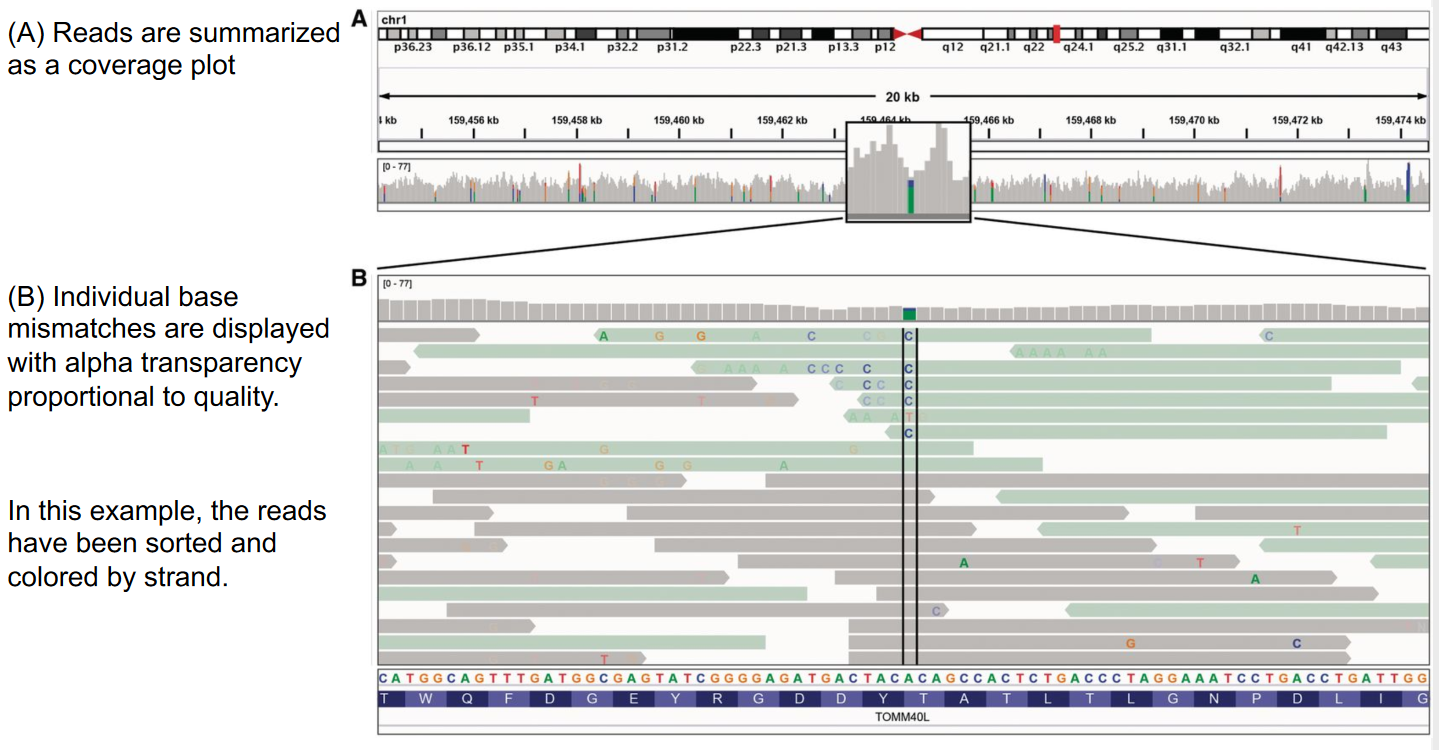
\includegraphics[width=0.6\textwidth]{IGVReadsView.PNG}
    \label{ViewReads}
\end{figure} 


\subsection{Igvtools}
Igvtools comprises a set of utilities for preparing large files for efficient display.

\begin{figure}[H]
    \caption{igvtools possible operations, the "count" function allows to generate coverage data, and it takes in input a BAM file. The obtained data could be then loaded with the "Load pre-computed coverage data" commandq}
    \centering
    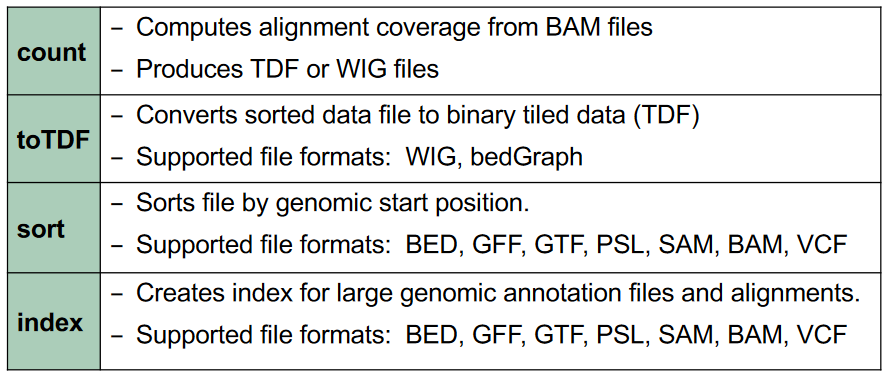
\includegraphics[width=0.6\textwidth]{igvtools.PNG}
\end{figure}

\subsection{Session Files}
Sessions are an integral part of IGV, allowing users to share their data and
views with other users simply and accurately. Session files describe the session
in XML.

\begin{figure}[H]
    \caption{Structure of the XML file}
    \centering
    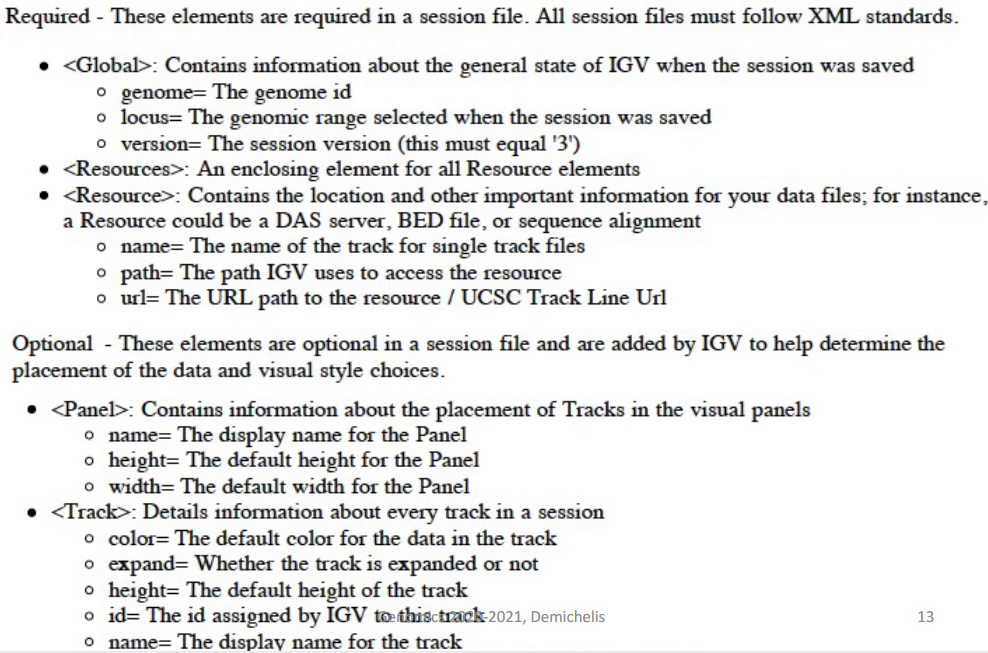
\includegraphics[width=0.75\textwidth]{structureXMLfile.PNG}
    \label{XMLfile}
\end{figure} 



\section{Some of the main utilizations}
\textit{(I will not write down all the passages needed to obtain the figures represented
below, as they are included in the exercise file delivered by the professor)}

\subsection{RNA-seq alignments}

\begin{figure}[H]
    \caption{the height depends on the quantity of reads connecting the different exons.}
    \centering
    \includegraphics[width=0.6\textwidth]{RNAseqAlign.PNG}
\end{figure}

\begin{figure}[H]
    \caption{\textbf{Sashami plots}: The number of reads connecting exosomes are
    represented here on the curved lines. The peaks represent coverage within
    exons.}
    \centering
    \includegraphics[width=0.6\textwidth]{sashamiplot.PNG}
\end{figure}

\subsection{Study of variants}
It is possible to study variants from different samples.

\begin{figure}[H]
    \centering
    \includegraphics[width=0.6\textwidth]{variantsView.PNG}
\end{figure}

It is also possible to sort the samples in different ways and to group them considering different characteristics.



\section{Exercise}

The goal was to read pairs/end order/coverage/insert sizes at following
coordinates (hg19). Interpret, if possible, as inversion, inverted duplication,
tandem duplication, or deletion.

\begin{figure}[H]
    \caption{\textit{\textbf{chr1:11,050,009-11,055,137}}: It could be a tandem duplication on one of the two alleles and a deletion on the other allele. The reason why I would suggest the presence of a deletion is due to the fact that the coverage remains quite constant, despite of the duplication.}
    \centering
    \includegraphics[width=0.6\textwidth]{pos1.PNG}
\end{figure}

\begin{figure}[H]
    \caption{\textbf{\textit{chr5:9,410,315-9,413,699}}: it is quite clear that both the alleles were deleted in that region, because of the decrease in coverage}
    \centering
    \includegraphics[width=0.55\textwidth]{pos2.PNG}
\end{figure}

\begin{figure}[H]
    \centering
    \begin{subfigure}[t]{0.6\textwidth}
        \centering
        \includegraphics[width=1\textwidth]{cov3.PNG}
    \end{subfigure}
    \begin{subfigure}[t]{0.6\textwidth}
        \centering
        \includegraphics[width=1\textwidth]{pos3.PNG}
    \end{subfigure}
    \hfill
    \begin{subfigure}[t]{0.6\textwidth}
        \centering
        \includegraphics[width=1\textwidth]{pos3passages.jpg}
    \end{subfigure}
    \caption{\textit{\textbf{chr7:31,576,117-31,599,940}}: Basically you have an inversion between B and F, and after the deletion of the ED portion, the other allele remains normal.}
    \label{fig:3}
\end{figure}

%#TODO complete all the figures of the exercise
%#TODO it could be a good idea to expand this part with some information. Let me know.


\graphicspath{{chapters/TumorEvAndVesciclesImages/}}


\chapter{Tumor evolution studies via NGS data}

\textbf{\textit{Written by Stefano Cretti}}


\section{Why studying tumor evolution?}

  Understanding tumor evolution is useful for: 
  \begin{itemize}
    \item \textbf{Academical purpose}; mainly for research
    \item \textbf{Clinical purpose}; the order of somatic events during tumor
    evolution can be relevant when considering the management of a patient, e.g.
    it can affect the treatment decided by the tumor board. A \textbf{tumor
    board} is an organism present mostly in research oriented ospitals (but also
    non research oriented ones and its popularity is increasing), and it is
    composed by different specialists (oncologist, genetist, radiologist,
    comutational biologist, pathologist and others) which manage the patients
    jointly. Aside from clinical purposes, this organism is also useful for
    training new experts. 
  \end{itemize}


\section{Tumor heterogeneity}
  
  A tumor can arise due to strong driver mutations or because of the
  accumulation of several minor alterations. In both cases the mutations are
  \textbf{somatic events} due to stochastic processes, mainly due to
  carcinogenic substances that damage DNA therefore causing mutations (but also
  physcal phenomena such as radiations and others). These mutations are mostly
  associated to cell growth; this is why tumor cells often undergo clonal
  expansion and create a mass. The \textbf{speed} at which the mass grows and
  mutates is dictated by the mutations that occurred. \\
  
  A tumor mass can be either \textbf{homogeneous or heterogeneous}; in general,
  the more aggressive and old the tumor is, the higher the degree of
  heterogeneity. Higher heterogeneity usually correlates to drug resistance
  (since some of the clonal populations might be able to better resist the drug
  compared to others).\\

  \textbf{New Generation Sequencing }allows to study all the somatic mutations
  that occurred in a cell, both the cancer related ones and the benign ones. By
  sequencing with an appropriate depth, you can infer in which fraction of the
  cell population a certain mutation is present; this allows to reconstruct the
  \textbf{clonality} of the tumor and the mutation history. Notice that since
  very deep sequencing can give errors, you usually need to check different loci
  in order to consolidate your result. \\

  % To add definitions, remember to put in the prefix the command
  % \newtheorem{definition}{Definition}
  \begin{definition}
    \textbf{Clonality}: the characteristic of the tumor to expand clones of
    itself (written by Maurizio). Since tumor's behaviour could be considered
    related to the behaviours of the tumor clones, it is possible to assess
    clonality of some modifications, and relationships between them
    (subclonality). Clonality becomes also a measure of the abundance of a
    specific alteration, by evaluating the dimension of the related cellular
    clone.
  \end{definition}

  Tumor heterogeneity can be subdivided into: 
  \begin{itemize}
    \item \textbf{Inter-individual heterogeneity}: tumor from patient A is
    different from that of patient B.
    \item \textbf{Intra-individual heterogeneity}: tumors from the same patient
    might differ
    \begin{itemize}
      \item \textbf{Spatial heterogeneity}: synchronous tumor masses in the same
      patient might differ.
      \item \textbf{Temporal heterogeneity}: a tumor might changes overtime, due
      to spontaneous or drug induced selection.
      \item \textbf{Intra-lesion heterogeneity}: an individual tumor mass might
      present different lesions (which display different clones with different
      mutations, therefore different phenotypes, treatment resistances and so
      on).
    \end{itemize}
  \end{itemize}
  Almost always, many of these heterogeneities are present simultaneously. \\
  
  Notice that\textit{ genetic heterogeneity does not necessarely reflect
  morphological} heterogeneity (e.g. different prostate lesions might look the
  same when stained but then display different markers using in situ
  immunochemistry). Moreover tumor mass size does not necessarely correlate with
  \textbf{aggressiveness} (hence imaging is not enough to study tumors).
  Heterogeneity might cause problem in the interpretation of the spectrum
  obtained via sanger sequencing, since the sample might contain different
  sequences for the same locus, hence leading to an overlap in the peaks. In
  case of different lesions, we can define tumor burden and features of each of
  them via individual sequencing.

  \begin{definition}
    \textbf{Tumor burden} refers to the number of cancer cells, the size of a
    tumor, or the amount of cancer in the body. Also called tumor load.    
  \end{definition}
  
  Tumor evolution can happen in two ways (figure \ref{fig: tumor evolution}):
  \begin{itemize}
    \item \textbf{Linear evolution}: genetic instability leads to new tumor
    clones and if those display some advantage compared to the previous ones,
    the older ones get replaced by the new ones (otherwies the new clone dies
    down). In this case you generally have low heterogeneity. 
    \item \textbf{Branched evolution}: genetic instability leads to the
    formation, from an ancestral clone, of different clonal populations which
    can coexist in the same or different tumor masses. In this case you
    generally have high heterogeneity.
  \end{itemize}

  \begin{figure}[ht]
    \caption{difference between linear evolution and branched evolution. In the
    first case, advantageous mutations are accumulated by the same cell
    population. Instead, in the second, several subpopulations originate and
    those develop differently, maintaining a common ancestor}
    \centering
    \includegraphics[width=0.9\textwidth]{image_09.PNG}
    \label{fig: tumor evolution}
  \end{figure}
  
  A \underline{\textbf{metastasis}} can either have:
  \begin{itemize}
    \item \textbf{Monoclonal origin}: meaning that it originates from tumor
    cells coming from a single lesion. In this case you have similar features as
    the starting mass and overall low heterogeneity within the metastasis.
    \item \textbf{Polyclonal origin}: meaning that it originates from multiple
    tumor cells coming from different lesions. This phenomenon is called
    \textbf{multiclonal seeding} and it leads to high lesion heterogeneity.
    Moreover, the fact that it displays some of the features from each of the
    parental lesions makes the analysis more complex.
  \end{itemize}
  
  As previously mentioned, tumor heterogeneity plays a big role in defining
  treatment resistance. We talk about two types of drug resistance (figure
  \ref{fig: tumor resistance}):
  \begin{itemize}
    \item \textbf{Primary resistance}: the pre-treatment tumor mass already
    contains cells that are resistant to the treatment; the treatment kills the
    non-resistant cells, hence the resistant clone expands. 
    \item \textbf{Acquired resistance}: the pre-treatment tumor mass does not
    already contains cells completely resistant to the treatment; the clones
    that can survive the treatment the best could then mutate in order to
    acquire a treatment immunity mechanism. 
  \end{itemize}

  \begin{figure}[H]
    \caption{Primary resistance against acquired}
    \centering
    \includegraphics[width=0.6\textwidth]{image_08.PNG}
    \label{fig: tumor resistance}
  \end{figure}

  In case of primary resistance, the tumor might already display some biomarkers
  pointing to some treatment resistance; this is useful for the tumor boards in
  order to avoid needless harmful treatments. However, no biomarkers for each
  treatment are known, plus the tumor can always evolve unpredictably and
  acquire a new resistance. 


\section{Algorithms to study tumor evolution}
  
  You can study tumor evolution using information from:
  \begin{itemize}
    \item Samples from the \textbf{same subject}, from different time points or
    lesions; this way you can reconstruct mutation order and metastatic
    processes within the individual (base on shared or not mutations). 
    \item Samples from \textbf{different subjects} affected by the same
    pathology (e.g. prostate cancer); you use recurring patterns across
    individuals, this way you can reconstruct more generic features of the
    pathogenesis, for instance:
    \begin{itemize}
      \item Very common mutations in the pathology (those shared across many
      individuals)
      \item Mutations that tend to happen in a specific order (take for instance
      two mutations \textit{A} and \textit{B}; if in the majority of tumors
      which present both lesions, \textit{B} is almost always subclonal to
      \textit{A}, then probably \textit{A} tends to happen prior to \textit{B}).
    \end{itemize}
    \begin{figure}[ht]
      \caption{Tumor evolution time using samples from different individuals}
      \centering
      \includegraphics[width=1\textwidth]{image_10.PNG}
      \label{fig: tumor evol algorithm}
    \end{figure}
  \end{itemize}

  For more in depth reading (clickable links):
  \begin{itemize}
    \item \href{https://pubmed.ncbi.nlm.nih.gov/25830880/}{\textit{The
    evolutionary history of lethal metastatic prostate cancer, Gundem et al,
    Nature 2015}}
    \item \href{https://pubmed.ncbi.nlm.nih.gov/23622249/}{\textit{Punctuated
    evolution of prostate cancer genomes, Baca et al, Cell 2013}}
  \end{itemize}
  In general, when you have some tumor data, you try to see which of your models
  best fits the progression. \\

  There are \textit{several aspects that must be taken into account during this
  type of analysis}; most of them are useful in comprehending the pathology and
  its mechanisms, but at the same time they make analyzing the NGS data more
  difficult. Some of these aspects are: \textbf{Heterogeneity} (inter-patient,
  intra-patient, intra-tumor), \textbf{Time dependence} (tumor changes
  overtime), \textbf{Treatment status} (was the tumor treated, if yes how?),
  \textbf{Admixture DNA} (presence of non-tumoral DNA)
  
  \begin{definition}
    In a tumor biopsy you could have (and this is generally the case) other
  cells that are not tumoral (healthy tissue cells, stromal cells,
  leukocytes...). It is then defined the concept of \textbf{admixture}, which is
  \textit{the fraction of non-tumoral DNA within the sample}. Admixture is then
  used to define \textbf{tumor purity}, which is
  $$
  \text{tumor purity } = 1 - \text{ admixture}
  $$
  \end{definition}
  To sum up, a fully tumoral sample would have admixture equal to zero and
  purity equal to one. The opposite holds for healthy tissue (purity equal to
  zero, admixture equal to one). Deconvoluting the sequences derived from
  admixed DNA complicates NGS data analysis, but also provides useful
  information:
  \begin{itemize}
    \item Aggressiveness of a lesion; in general, the lower the purity, the
    better the outcome
    \item Defining whether a mutation is actually part of a subclonal tumor
    population or it is just admixed DNA
  \end{itemize}
  
  The most useful \textbf{features from NGS for characterizing tumor evolution}
  (clonality, purity and so on) are:
  \begin{itemize}
    \item Copy number mutations
    \item Point mutations
    \item Single cell sequencing
    \item Polymorphic information (which SNPs does the tumor have). The
    algorithms used to study tumor evolution use \textbf{informative SNPs},
    meaning:
    \begin{itemize}
      \item SNPs for which the individual is heterozigous (hence they vary from
      individual to individual)
      \item SNPs for which the allelic fraction is easily measurable \\
    \end{itemize}
  \end{itemize}

  
  Making \textbf{parsimonious} assumptions (mainly that all clones have the same
  growth rate), these algorithms allow to study any form of genetic aberration.
  \\

  In order to quantify the variability of tumors, it is possible to exploit the
  minor allele frequency and allelic fraction quantifications.
  \begin{itemize}
    \item \textbf{Minor allele frequency}: Minor allele frequency (MAF) is the
    frequency at which the second most common allele occurs in a given
    population.
    \item \textbf{Allelic fraction}: Proportion of reads supporting the
    alternative base.
    $$
    \text{Allelic fraction} = \frac{\text{locus reads with counted allele}}{\text{total locus reads}} 
    $$ 
    The \textbf{allelic fraction} for an informative SNP can be:
    \begin{itemize}
      \item 0 if the alternative allele was deleted
      \item 1 if the reference allele was deleted (the non-alternative one)
      \item Around 1/2 if both alleles are present in equal proportion
      \item Some other value in the range (0,1), that could be due to
      duplication, heterogeneity (admixture and/or subclonality), errors and so
      on. In this case some further information might be required (for instance
      the coverage)
    \end{itemize}

    \item \textbf{Neutral reads}: reads equally representing parental
    chromosomes. Neutral reads are quantified through Beta fraction.
    \textbf{Beta fraction}: percentage of neutral reads. Beta goes from 0 to 1;
    the closer the value to 1, the closer the reads are to a 50/50 split among
    parental sequences, the closer the value to 0, the closer the reads are to a
    100/0 split in favour of either parental sequence. The \textbf{beta
    fraction} can be:
    \begin{itemize}
      \item 0 if either allele was deleted (hence you have only one)
      \item 1 if both alleles are equally-represented (normal condition)
      \item Any other value in the range (0,1), and this is also due to
      heterogeneity and other factors.\\
    \end{itemize} 
  \end{itemize}

  \textbf{Using allele frequency and beta fraction, informative SNPs} can be
  used to reconstruct the genealogy of the mutations. If there is a deletion of
  a region then you have a \textbf{loss of heterozygosis} for all SNPs in that
  region (since you chose informative SNPs, hence heterozygous ones); then based
  on the mutations present or absent in the different clones of the lesion
  (since you do not have a perfectly homogeneous mass) you can reconstruct their
  order.  

  When designing a test you need multiple informative SNPs for each genomic
  fragment of interest. Moreover you have to choose \textbf{alleles that have
  high MAF} (hence the minor allele frequency is still rather high), since those
  are more likely to give you information. 

  For more in depth reading (clickable links):
  \begin{itemize}
    \item \href{https://pubmed.ncbi.nlm.nih.gov/31524989/}{\textit{Ploidy- and
    Purity-Adjusted Allele-Specific DNA Analysis Using CLONETv2, Davide Prandi,
    Francesca Demichelis, 2019}}
  \end{itemize}

  \begin{figure}[H]
    \caption{(A) Example of the allelic fraction (AF) and beta ($\beta$) values
    as computed in five genomic positions (p1 to pm) corresponding to five
    informative SNPs. Positions p1 to pn are within a hemizygous deleted genomic
    segment A, while genomic positions pn+1 to pm lie within a wild type genomic
    segment B. (B-D) Examples of a normal cell and two different tumor cells.
    Tumor cells 1 and 2 differ in the status of genomic segment B. Histograms
    below the cell cartoons report the expected distribution of the AF of SNPs
    in genomic segments A and B together with the associated beta values. (E-F)
    Examples of two different tumor samples. Tumor sample 1 includes one normal
    cell and nine tumor cells with deleted genomic segment A and wild type
    genomic segment B. Tumor sample 2 differs from tumor sample 1 in the
    presence of six tumor cells with a hemizygous deletion of genomic segment B.
    Expected distribution of the AF of informative SNPs together with estimated
    $\beta$ are depicted below each tumor sample cartoon.}
    \centering
    \includegraphics[width=0.7\textwidth]{image_01.jpg}
    % \label{fig: }
  \end{figure}


\section{Estimating admixture and clonality}
  Notice that the beta fraction correlates with the shape of the distribution of
  the allelic fractions of the informatives SNPs in the read;\textbf{ with
  $\beta$ = 1, you have a normal distribution with mean 0.5, with $\beta$ = 0
  you have two sharp peaks at 0 and 1, with any intermediate value you have to
  peaks which can be partially overlapping for values close to 1}. Notice that
  increasing the coverage does increase the resolution of the peaks. For this
  reason increasing the coverage (with beta constant) does increase the ability
  to distinguish clonality, especially of populations that are only some degree
  of difference from each other.
  
  \begin{figure}[H]
    \caption{As $\beta$ increases, the peaks become wider and go towards the
    center of the graph. With higher values of coverage, given the same $\beta$,
    peaks (involving the two possible variants) become more distinguished.}
    \centering
    \includegraphics[width=0.75\textwidth]{image_02.jpg}
    % \label{fig: }
  \end{figure}

  To \underline{\textbf{estimate the admixture/clonality}} of a cell population:
  \begin{itemize}
    \item Measure the \textbf{allelic fraction and beta fraction of each
    informative SNP} of a genomic region
    \item For each region try which of the models \textbf{fits your data the
    best} (basically map the distribution of the allelic fractions of the region
    against prefitted reference distributions) 

    % #TODO Questo significa trovare un riferimento adeguato? in che senso?
    \item You can then compute the local and the global admixture:
    \begin{itemize}
      \item \textbf{Local admixture} (calculated on a part of the sample) is a
      measure of the fraction of cells displaying a certain lesion; for this
      reason local admixture is used as an estimate for $\rightarrow$
      \textbf{clonality}
      \item \textbf{Global admixture} is a measure of how many cells, on
      average, have a lesion; this can be used to estimate the $\rightarrow$
      \textbf{DNA admixture} (purity) of the sample
    \end{itemize}
  \end{itemize}
  Hence this technique allows you to distinguish purity and subclonality.
  
  Graphically you obtain a plot with:
  \begin{itemize}
    \item On the x axis, the cromosomal coordinates indexed by informative SNPs.
    The longer the horizontal segment, the bigger the considered region. 
    \item On the y axis, the MAF values for the informative SNPs. Any drop below
    the 0.5 value means that the region does not have a 50/50 split (in fact, a
    MAF value of $0.5$ means that the minor allele is present in 50\% of the
    reads, as the "reference" allele). The deeper the drop the deeper the
    difference in the representation of the alleles. 
  \end{itemize}

  \begin{figure}[H]
    \caption{ Top subplot: represents the MAF distribution of a clonal cell
      population. In all the local cases drops in MAF are present also in the
      reference sample; Bottom subplot: local changes in MAFs do not mirror
      properly those present in the reference sample }
    \centering
    \includegraphics[width=0.9\textwidth]{image_03.jpg}
    \label{fig: local globla admixture}
  \end{figure}

  In the example picture \ref*{fig: local globla admixture}, the top subplot
  shows drops which have very similar depth, hence global and local admixtures
  are similar and there is very low heterogeneity. In the bottom subplot you
  have differences in local and global admixtures, hence we can infer the
  presence of different clonal populations. 
  
  For this type of analysis is always useful to have the \textbf{match normal
  DNA} (the non-tumor DNA of the subject): match normal DNA is usually obtained
  from leukocytes in the blood, otherwhise one could somehow deconvolute the
  signal of the admixed cells. \\

  Another graphical representation in bidimensional space is the following plot
  (figure \ref{fig: log2 plot}):
  \begin{itemize}
    \item On the x axis the \textbf{log2 ratio}, meaning 
      $$
      \text{log2 ratio} = \log_2\frac{\text{local tumor coverage}}{\text{local normal coverage}}
      $$ 
      This indicates how abundant cancer DNA is with respect to healthy DNA
      (gain of DNA if above zero, loss of DNA if below zero).
    \item On the y axis the \textbf{apparent admixture}, which is a measure of
    subclonality and is defined as
      $$
      \text{Adm. apparent} = \frac{\beta}{2 - \beta}
      $$
      Notice that this measure refers to each individual deletion/abnormality.
    \item The dots which represent the individual genomic segments. The dots
    tend to create multiple clusters and the closer two points are, the more
    probable the events they represent are close to each other in time. when
    dots are in a same cluster it means that they very likely share the same
    copy number status and also the same level of clonality.
  \end{itemize}
  
  \begin{figure}[ht]
    \caption{log2 ratio representation: when beta is equal
    to 1 the concept of admixture (1-purity) is equal to 1 meaning that purity is
    equal to 0 if we are at the top of the y scale it means that there's no signal
    related to tumor content, while the lower we go, so the closer we get to 0, the
    higher the tumor content and the level of clonality is. We have losses and
    gain of DNA copies, moving on the x axis.}
    \centering
    \includegraphics[width=0.6\textwidth]{image_04.png}
    \label{fig: log2 plot}
  \end{figure}
  
  You can compute clonality using the formula:
  $$
  \text{clonality} = \frac{1 - \text{Adm. apparent}}{1 - \text{Adm. global}}
  $$

  An example of how heterogeineity can lead to difficult to interpret results
  can be found in the following paper:
  \href{https://pubmed.ncbi.nlm.nih.gov/25160065/}{\textit{Unraveling the clonal
  hierarchy of somatic genomic aberrations}}. \\



\graphicspath{{chapters/TumorEvStudiesIIImages/}}

\chapter{Tumor evolution studies (continued)}


\section{Recalls from the previous lecture}

At the basis of tumor evolution is the concept of how to use {informative SNPs}:
SNPs for which a specific individual has heterozygous calls so that set of SNPs
is unique for every individual.

This property is connected to the fact that when we have the loss of an allele,
the allelic fraction of the informative SNPs within that lesion will be
informative of the lesion and its depth (clonality = what's the fraction of
tumor cells that very likely harbor that lesion).

We can also have different population of cells, when a set of lesions is present
in every population it is said to be clonal whereas when a specific set of
lesion is harbored only by a subpopulation it is defined as subclonal.

\includegraphics[width=2.37708in,height=2.94375in]{image1.png}\emph{Estimate of
DNA Admixture}

\emph{{Log2 Ratio}} is the log2 of the ratio of the tumor over the normal that
applies to array data signals (intensity of the signals) but also to the local
coverage of a tumor BAM file over a normal BAM file.

In the figure each dot is a genomic segment or a gene that clusterize in the
space and when dots are in a same cluster it means that they very likely share
the same copy number status and also the same level of clonality.

\emph{{Beta}} is a variable that goes from 0 to 1 and provides information of
the number of reads that equally represent the two alleles; when beta is equal
to 1 the concept of admixture (1-purity) is equal to 1 meaning that purity is
equal to 0 if we are at the top of the y scale it means that there's no signal
related to tumor content, while the lower we go, so the closer we get to 0, the
higher the tumor content and the level of clonality is.

If we use this equation we can assess the level of clonality of a cluster.

So the graph in the figure puts in relation the copy number status (log2 ratio)
and the purity/clonality of the sample (Beta); the more we go towards the left
the fewer number of copies, the lower on the y axis the higher the clonality.

The best proxy of the quantity of tumor content present in a sample is done
using the lowest cluster.

\includegraphics[width=3.46875in,height=2.65139in]{image2.png}We have losses and
gain of DNA copies, moving on the x axis.

The beta is related to the clonality so the lower we go the more clonal the
signal is.

The only difference from the previous figure is the presence of extra clusters:

\begin{itemize}
\item
  The blue cluster with deletions is the most clonal one
\item
  Both blue and green clusters had deletions, since they have a negative log2
  ratio, but the green ones are less clonal than the blue ones
\item
  In log2 R = 0 and ß = 1, where there's the red cluster, we have a status of no
  copy number changes (wild-type status in terms of copy numbers). This
  basically represents a total number of alleles which is the same in both the
  tumor and normal sample.
\item
  All the other clusters with a positive log2 ratio had a gain of DNA
\end{itemize}

\includegraphics[width=2.72153in,height=2.08958in]{image3.png}

In this figure the number of copies that correspond to all the clusters in the
space is also reported.

\begin{itemize}
\item
  Blue one: one copy of DNA, so we have a deletion
\item
  Green one: also one copy of DNA but with subclonality
\end{itemize}

This is how we can map in the space the status of clonality and the number of
copies for a specific segment in the genome.

So again, the lower we go the more clonal the clusters are, the more left the
deeper they are in terms of loss of DNA.

We can use these information to build \emph{{evolution maps}}.

The first thing to do is to look, within each individual, at concomitant
deletion where one is subclonal to the other one.

\includegraphics[width=3.18859in,height=2.21348in]{image4.png}

In the figure:

\begin{itemize}
\item
  In sample 1 the brown lesion is subclonal to the orange one, and that same
  lesion is also subclonal to the green one.
\item
  In sample 2 we have again the support of the relation between the brown and
  orange lesion with the same level of subclonality (brown subclonal to orange).
\item
  In sample 3 is the same as in sample 1 and 2.
\item
  Samples 4 and 5 have the same concomitant green and brown lesions again with
  the same level of subclonality.
\item
  In sample 5 only we also have another concomitant lesion (blue subclonal to
  brown).
\end{itemize}

So we perform this analysis for all the concomitant lesions in our sample and we
start drawing the arrows to keep track of what is subclonal to what. We compile
this list across all individuals and look for how many times we see support for
the same relationship in the same direction.

In our case we can say that the relationship going from orange to brown is
supported by 3 out of 5 individuals; the same can be said for the green going to
brown. The blue one is instead not significant since it's supported by only one
individual.

So having multiple observation supporting that aberration x precedes aberration
y (i.e. aberration y is subclonal to aberration x) we can build an evolution
chart.

\includegraphics[width=2.38194in,height=2.40417in]{image5.png}

The orange and the green which have no relationship between them, are at the
same level on the x axis in the path and they both go into brown.

So one can assume that the more clonal a lesion is the more likely it is that it
occurred earlier during the evolution (time is on the x axis of the path), and
we can look for recurrent relationships among lesions.

In principle we can say that the grey ones at the beginning happened at the same
time point and then at a second time point, the tumors in our set of samples,
underwent loss of orange and green genes and then later they both underwent loss
of the brown gene.

\includegraphics[width=2.63403in,height=1.74097in]{image6.png}If we do that in
large datasets (lung cancer melanoma, prostate cancer \ldots) we can come up
with all the dependencies that were observed and that were supported by more
than one individual (e.g. in prostate cancer we can say that a loss in NKX3-1
precedes the deletion of PTEN).

Even if we have hundreds of BAM files on whole exon sequencing data from large
collections all that we can build are evolution maps with at most three layers
(pretty disappointing).

This has multiple reasons, one of them is that:

\begin{itemize}
\item
  To build a relationship which is statistically significant between two genes
  we need to have multiple instances of that relationship (in many samples)
  which means that we need to have co-occurrence of the two lesions and
  subclonality of the second lesion with respect to the first in a significant
  number of individuals compared to the total number of individuals that have
  co-occurrence. So if co-occurrence occurs in N individuals and subclonality of
  the second lesion to the first one occurs in a fraction of those, only if this
  fraction is significant with a proportion test out of the total number, then
  we can build the path.
\end{itemize}

Therefore we are tremendously limited by co-occurrence of lesions.

To boost the reconstruction of these paths gene families or pathways have been
exploited.

E.g. if we are dealing with PTEN which is a tumor-suppressive gene relevant in a
specific pathway (PF3K), then it doesn't matter if we have deletion or
inactivation of the same genes in the same pathway, what matters for the tumor
evolution is that that specific pathway is altered and so what we can do is
start aggregating signals from genes that belong to the same pathway.

So if individual 1 has a relationship between gene A and some gene in a specific
pathway (PF3K) and individual 2 has a relationship between gene A and a second
gene in that same pathway, then we can assume that maybe they have the same
effect and so we can aggregate the information on the landing gene.

So instead of going from gene 1 to gene 2 we go from pathway 1 to pathway 2, and
in terms of numbers what we gain is that the co-occurrences are counted
including all the gene lesions with the same function in pathway 1 and all the
gene lesions with the same function in pathway 2 (if we consider the
inactivation of the gene then we have to consider all the lesions that
inactivate the gene and not others).

We can then run a simple test to build our path.

With this method we start having some more data to look for major changes during
the evolution of the tumor pathway.

E.g. in prostate cancer we'd identify a set of pathways that are more or less at
some level altered in earlier staged disease and that then trigger or are
precedent to our pathways. Doing so we can learn more in terms of the biology of
the disease evolution.

We can also decide to go for a mix model or a mix approach, where for certain
genes we go at the pathway level while for other we treat them separately.

There are also more complicated ways to make inference of tumor evolution. Some
try to avoid the hypothesis that the more clonal a lesion is the more likely it
is to happen early, because we know it's not always the case; it might be in
untreated samples but not in treated samples. In a treatment regiment, because
of drug pressure selection, specific resistant clones harboring a specific
lesion can take over due to their higher rate of proliferation, so in this case
if we see a lesion that appears to be more clonal it doesn't really mean that it
happened earlier, it may be that it had a higher proliferation and so it's
taking over (and we see it as apparently clonal but it's in fact a late event)
-\textgreater{} important concept in precision medicine.

So simplicistic approaches like the one discussed are proper for untreated (in
terms of drugs) primary diseases.

Evolution charts can also be boosted via the combination of multiple molecular
layers.

\section{Ploidy and purity correction on $\log_2(\frac{T}{N})$ data}

\emph{How can we use measure of the tumor purity and the effect of the tumor
ploidy?}

\emph{How can we compare two different samples for which we quantify completely
different levels of tumor content?}

E.g.: we have a sample a 100\% pure and with 50\% of clonality (a lesion present
in 50\% of the cells) and a second sample with a tumor purity of 10\% and a
clonality of 100\% (a lesion present in 100\% of the cells), we need a way that
allows us to compare numbers without having to convert everytime for every
lesion the depth of the lesion based on the tumor content, so we need an
equation that we can apply to every individual data that puts everything on the
same level

(same concept as gene expression normalization).

The coverage makes data coming from different samples comparable because we
normalize everything to the total coverage, but when we deal with diseased cells
we can have contamination from the admixture, so we need an extra step.

The step, once we know how to assess the tumor purity and ploidy, is quite
simple: we need to adjust the data for tumor purity and ploidy.

\emph{Schematically}\includegraphics[width=3.79931in,height=5.42569in]{image7.png}

In the figure we are looking at one tumor sample: a whole genome sequencing of
one melanoma sample.

We see multiple peaks which correspond to different copy number states.

Let's suppose we have a genome with a backbone of three copies but we sequence a
bulk and we don't have 100\% purity but 80\% (so 20\% is contamination).

\emph{\textbf{Ploidy correction}}

Computationally we assess the ploidy through the copy number space and then
correct the data.

From the tumor and the normal we obtain something like the first graph, and we
could wrongly assume that the main peak is always in 0 (wild-type state of the
genome), but it shouldn't.

In fact, if we assess the ploidy and overall we see a backbone state of three
copies for our genome, then the main peak should be shifted toward three.

So, the \emph{ploidy correction shifts the distribution} towards the right
(second graph).

\emph{\textbf{Purity correction}}

We correct our data and the \emph{{purity correction causes a stretch between
the peaks}}, since tumor admixture dilutes the signal. So, the effect of purity
correction is a wider spread between the peaks (third graph).

+ add the example graph

\begin{itemize}
\item
  If we have one extra copy in our tumor, the log2 ratio will be around 0.58 and
  so we would expect that the signal will peak around that value; for two extra
  copies we'd expect a peak around 1 and so on.
\item
  We'll have the peak of the normal state around 0 and then if we have an
  underrepresented allele in our tumor we'd get another peak around -1 for the
  hemizygous deletion and then the homozygous deletion.
\item
  If our signal is not 100\% pure tumor (so diluted by normal cells), the peak
  at -1 and 0.5 would be closer to the 0 peak for uncorrected data.
\end{itemize}

\emph{{When we correct for tumor purity we stretch the distribution to go to the
correct positions.}}

E.g.: 25 whole genome sequencing of melanoma samples

\includegraphics[width=3.42917in,height=4.56111in]{image8.png}

\begin{itemize}
\item
  1\textsuperscript{st} graph: The distribution of the log2 data of uncorrected
  signal, every melanoma sample is highly aberrant with a ploidy that is
  different between different individuals and a purity that is also different
  between different individuals. But we do have the tumor ploidy and purity so
  we can correct the data.
\item
  2\textsuperscript{nd} graph: we correct for ploidy
\item
  3\textsuperscript{rd} graph: we correct for purity too
\end{itemize}

If we don't correct our data we'll see much noise (as in the first graph).

From the corrected data we learn that:

\begin{itemize}
\item
  A lot of tumors have a backbone ploidy of two
\item
  There are some hemyzigous deletion not perfectly centered in one but closer to
  one in the 3\textsuperscript{rd} graph if compared to the
  1\textsuperscript{st}
\item
  Some signal is compatible with homozygous deletion
\item
  Whave a reasonable amount of signal for three copies which could come from a
  threeploid status of some tumors.
\end{itemize}

These corrections are part of standard preprocessing.

\emph{\textbf{Tumor Ploidy and Purity adjustment, corrected TCGA data}}

\emph{How commonly does suboptimal tumor purity affect proper copy number data
analysis?}

\emph{How common it is that purity is not equal to 100\% and ploidy is not equal
to 2 in any primary disease}

\includegraphics[width=3.24375in,height=3.97569in]{image9.png}

In the figure we can see a list of tumor types, where every draw is a tumor type
(lung carcinoma, bladder cancer, colon cancer, ovarian ecc.). On the x axis we
have tumor purity (1-admixture) going from 0 to 100\% and for each type we can
see the distribution of the tumor purity analysis of all the samples from the
TCGA dataset.

Every tumor type has a different number of sample profile

Looking at the GBM (glioblastoma multiforme), the middle vertical line is the
median signal of the distribution, there are outliers shown and the black
horizontal line represents the interquartile range.

Altogether across 27 tumor types they were able to assess the tumor cellularity,
clonality and all in about five thousand of those, meaning that a great fraction
of those had some optimal data (very strict criteria)

\begin{itemize}
\item
  The majority of the median distributions are above 50 \%.
\item
  The overall tumor cellularity was almost 70\%.
\end{itemize}

\emph{If we look at ploidy: what is the fraction within each tumor type with a
ploidy significantly above two}?

In the graph they are sorted by decreasing percentage of tumors with a ploidy
higher than two; for example, for the first and second tumor type, more than 50
\% of the primary tumors have a ploidy status above two so either they underwent
whole genome duplication (4 or more copies) or at least we have three.

Then we have some tumors with very low ploidy (blue dots) where at least one
copy of the entire genome is completely lost -\textgreater{} low allele specific
ploidy assessment.

The figure shows what happens to data when we correct for ploidy and purity

\begin{itemize}
\item
  \includegraphics[width=3.65972in,height=3.76389in]{image10.png}On the y axis
  we have the log2 ratio
\item
  On the left side we have the raw data
\item
  On the right side the adjusted data
\end{itemize}

We can see where correction for ploidy and purity takes the signal.

Focusing just on the first half we can see that

we have the same noise we've seen for the melanoma uncorrected data.

\emph{The correction of the data results in the reclassification of 30\% of the
totality of the segments} (if we don't correct we have a wrong copy number
classification in 30\% of the cases)

Then there are certain copy numbers which are more or less affected by these
corrections.

What's interesting is that the correction led to the doubling of the homozygous
deletions that we were able to observe (these are very important because it
means that the proteic product won't be there at all).

\textbf{ALLELE SPECIFIC ANALYSIS (CNA, CNB SPACE)}

\includegraphics[width=3.12639in,height=4.35903in]{image11.png}

Thinking in terms of allele specific data:

\begin{enumerate}
\def\labelenumi{\arabic{enumi}.}
\item
  We have unadjusted signal
\item
  We adjust
\item
  Then we can go to the beta-log2 ratio space where we can see that the data
  underneath the peaks are belonging to specific clusters
\end{enumerate}

This suggests that by only looking at the log2 ratio we are unable to
distinguish the presence of clusters with different clonalities.

The most interesting information is the lower cluster (on the x=0 axis):

\begin{itemize}
\item
  Even when the T/N = 1 (tumor/normal ratio) what we can have is a status of one
  copy and one copy or something that equally gives a log2 ratio equal to 0 but
  which still represents copy neutral loss of heterozygosity (CN-LOH), so two
  copies on one allele and zero copies on the other.
\end{itemize}

+ example figures (will be added soon, I have to draw them)

1\textsuperscript{st} figure:

We have the loss of an allele on A so we'll have 2-1-2 copies

2\textsuperscript{nd} figure:

We have the same situation on allele A but allele B is doubled so we'll have
3-2-3 copies

So, in this situation, the gene x will have two copies but both of them coming
from the same allele (B).

Computing the log2 ratio in this situation we'll have the log2(2/2) which will
lead to the collocation on the 0 axis but on the lower part (due to the
clonality).

The log2-beta statuses allows us to distinguish the copy-neutral LOH.

Also for the gain is the same (three copies from the same allele and zero from
the other)

There are equations that allows us to go from here to a space where our
coordinates are the number of copies of allele A and number of copies of allele
B.\includegraphics[width=6.68889in,height=2.97633in]{image12.png}For four copies
we can have different combinations:

\begin{itemize}
\item
  2 copies of A + 2 copies of B,
\item
  3 copies of A + 1 copy of B
\item
  4 copies of A + 0 copies of B
\end{itemize}

The equations are not important, what's important is that once we have corrected
the data then we can shift our analysis up to the level of number of copies of
each allele for each gene.

\emph{Why is this important?}

E.g.: Let's imagine that for gene X we have one copy lost on allele A and a
point mutation on the allele B which leads to unfunctional product so full loss
of the protein.

If we instead are in the second case and the point mutation happened after the
duplication then we'll still have an allele functioning, whereas if it happened
before the duplication, we'd have again full loss of functional protein.

If we are able to distinguish the alleles we are able to also distinguish in
which situation we are (which means we can distinguish between what's functional
and what's not).

\begin{itemize}
\item
  \includegraphics[width=3.00903in,height=2.89861in]{image13.png}Extra graph
  with the same space allele a/ allele B where we can divide the space in terms
  of total number of copies and also what happens on both.
\end{itemize}

So, this whole computation allows us:

\begin{itemize}
\item
  To reclassificate copy number status in the space by shifting and stretching
\item
  To also assign a copy number A and B to every segment of the genome, which
  means to every gene
\end{itemize}

If we do that we can see that many of the segments that have a total number of
copies equal to two are in fact 2+0 and not 1+1. This means that there is a
significant fraction of the genome which is apparently wild-type but which
actually underwent loss from one an allele and a gain on the other. This event
is called copy-neutral loss of heterozygosity (CN-LOH).

Copy-neutral because the number of copies doesn't change but there's been loss
of heterozygosity.

From the TCGA data, they observed a relevant fraction of high copy number levels
(4-5 copies) which all came from the same allele (one allele was lost and the
other underwent multiple cycles of duplication).

\includegraphics[width=2.29167in,height=2.00347in]{image14.png}So, looking at
the copy number only we'd say there's a gain (which is true) but we wouldn't
have all the complete information (we also have to perform the allele analysis).

These information are relevant in precision medicine because there are ways to
target genes exploiting loss of heterozygosity and up until now it was only used
for deletions but now that's known, even if we have an apparent CN-LOH or we
have a copy number gain LOH we can still consider to use the same approach.

\includegraphics[width=6.58333in,height=5.0625in]{image15.png}\textbf{Case study
-- CNA, CNB real data example with multi-sample data from the same patient}

We have one patient and we're looking at a primary sample, for which we plot the
whole sequencing data in the copy number allele space and what we see (from the
first plot) is that:

\begin{itemize}
\item
  There's a cloud of dots (every dot is a gene) which has a total number of
  copies around two
\item
  There's a cluster that underwent hemyzygous deletion so we only have one copy
  of all the genes in there
\item
  There's one gene with a homozygous deletion (0,0).
\end{itemize}

Then we have three other metastatic sites for which they had biopsies so that
they could run whole genome sequencing and perform the analysis of the data in
the same space.

We have a local metastasis and two distant mets.

What we see:

\begin{itemize}
\item
  In distant met 1 there's no homozygous deletion*
\item
  In both the distant mets the gene RB1 gained an extra copy on allele A
\item
  In all the mets there are extra gains of copies of all the genes (maybe
  there's been a whole genome duplication of some sort)
\item
  In distant met 1 the data are as clean as to allow us to state that the data
  point in yellow/grey over the 1 is subclonal (if we have genes with 1+1 copy
  is equivalent to say it's a subclonal hemizygous loss, it means that all the
  cells have at least one copy and then some cells also have a second copy)
\item
  In terms of evolution, very likely extra copies of the whole genome also in
  the local met after the loss of the second copy of the gene
\item
  CN-LOH of many genes, including RB1
\item
  Level of subclonality overall not high
\end{itemize}

*\emph{How's possible that there's a homozygous deletion in the primary tumor
which is then absent in the distant mets?} No DNA can be regained, it's
impossible that the gene is reacquired, so probably the seeding of the distant
mets happened before the loss of the gene.

Another way to track evolution is to have \emph{serial time points.}

\includegraphics[width=6.68889in,height=5.05486in]{image16.png}

If we deal with biopsies over time we can track the evolution using the allelic
fraction of a lesion.

E.g.: reasoning in terms of point mutations, let's say we have a point mutation
at time point 0 in certain allelic fractions, which correspond to different
subsets, we track the fractions over time.

Doing this we can make inference of which subsets appear during the treatment
and are taking over (red one in the example figure).

Allelic fraction at any time point needs to be corrected for tumor content,
otherwise we would not be able to compare multiple time points from the same
patient.

\graphicspath{{chapters/TumorEvolution3Images/}}

\chapter{Tumor evolution studies via NGS data: SNVs-based methods}

\textbf{\textit{Written by Linda Cova}}

There is a large number of tumors where copy-number aberrations are minimal.
Consequently, it is difficult to use copy number based approaches for these
kinds of tumors. It is estimated that about 3\% of primary tumors present flat
genomes, meaning that they display very few copy number changes. These types of
tumors are correlated to a better prognosis both in overall survival and
progression-free interval, but relapses are still present so the assessment of
these tumors is important.

In order to address this issue, some tools were developed to detect tumor purity
via SNVs.

\section{Rationale of somatic point mutation based assays}

\begin{figure}[!ht]
\centering
    \includegraphics[width=0.5\linewidth]{peaks.png}
    \caption{\label{fig:peaks}Peaks shift for a clonal tumor cell population and
    some mixed populations. Considering two genomic locations, healthy cells
    have genotype AA-AA, clonal tumor cells AB-AA and subclonal tumor cells
    AB-AB, where B is the alternative allele associated with a somatic point
    mutation}
\end{figure}

The distribution of allelic fractions of the clonal population only is
symmetric, with the main peak around 0.5. A mixed population of clonal tumor and
normal healthy cells shows a shifted peak. The distance from 0.5 to the peak is
proportional to the fraction of normal cells, because normal cells contribution
moves the peak towards the side from the center (purity shift displayed in
\ref{fig:peaks}. A subclonal point mutation is identified with a second peak
towards 0, because its allelic fraction is probably far distant from 0.5.

\section{TPES (Tumor Purity Estimation)}
\textit{Alessio Locallo (Demichelis' student, 2019)}\\

\begin{figure}[!ht]
\centering
    \includegraphics[width=0.7\linewidth]{tpes.png}
    \caption{\label{fig:tpes}Workflow of the TPES algorithm}
\end{figure}

It is important to consider the \textbf{Reference Mapping Bias}: a polymorphic
locus carrying a non-reference base is less likely to be mapped during the
alignment process. With a perfect SNV (clonal, monoallelic, in highly pure
tumor), allelic fraction will not be 0.5 because the aligner considers the
variation as an error and sometimes discards the read containing it: some signal
is lost.\\

TPES steps:
\begin{itemize}
    \item \textbf{Selection of CN-neutral segments}: point mutations that are
    flat in terms of copy-number are perfect for flat genomes and easier to deal
    with. This is the first filter implemented by this tool: a threshold is set
    on the log2 of the tumor over the normal.
    \item When considering the \textbf{allelic fractions} of all the somatic
    mutations of whole genome, a major peak is expected around 0.5 (expected
    VAF). Other peaks can be originated from things that escaped the previous
    filter or from monoallelic mutations with copy-neutral LOH (loss of
    heterozygosity): in this case the allelic fraction results doubled. So
    another threshold on allelic fraction is needed (maxAF=0.55)
    \item Identification of \textbf{putative clonal SNVs}: the peak closer to
    0.5 is the most useful to determine tumor purity. The others are related to
    subclonal events.
\end{itemize}

With enough point mutations and after peaks identification, purity is assessed
with the following equation:
\[ 1-purity = admixture = 1-\frac{observedVAF}{expectedVAF} \]

\section{How many SNVs are needed to assess tumor purity?}

The number of SNVs changes for each tumor type, so not all tumor types guarantee
enough SNVs. The minimum number of SNVs needed to obtain reliable results can be
assessed with a \textbf{comparative analysis}. The Spearman's correlations
between the results of two different purity calling algorithms uding decreasing
number of SNVs are computed. The subsampling approach (which SNVs to consider?)
is to subsample the SNVs as many time as possible to have higher confidence on
the results. At each iteration, as many samples as possible are used, but the
number decreases when the number of SNVs increases.

The computations determined 10 as the minimum number of SNVs needed to infer
tumor purity. With this number, tumor was detected in 80\% of samples by
combining TPES and CLONET (CN-based). The 20\% could be tumor-free or not
detected samples. Since both SNVs and CN based methods failed, this 20\% could
be possibly detected with methylation.

\begin{figure}[!ht]
\centering
    \includegraphics[width=0.7\linewidth]{comparative.png}
    \caption{\label{fig:comp}\textbf{A}) Correlation between two purity
    estimating algorithms (TPES and CLONET) with decreasing number of SNVs
    considered. \textbf{B}) Percentages of samples where tumor purity was
    assessed by the two tools (TPES considering with 10 SNVs)}
\end{figure}


\section{Comparison between purity callers}

TPES was compared to other tools that do the same thing but with a range of
different methodologies: good correlation between the results was found, in
particular with the CN-based algorithms. This shows that genomics is more
reproducible in general to assess purity, while methods relying for example on
image analysis give different results.

The best solution to assess tumor purity is to couple and CN-based and a
SNV-based approach: some samples are only detected by one of the two so a
combination gives the best results globally.

\section{Pros and Cons of SNVs-based tumor purity assessment}
Pros:
\begin{itemize}
    \item Best-suited for CN neutral tumor genomes
    \item Applicable to a range of NGS techniques
    \item Fast and low demanding in terms of computational resources
    \item TPES is available as R package on CRAN
\end{itemize}
Limitations:
\begin{itemize}
    \item Needs a reasonable number of putative clonal somatic heterozygous SNVs
    per sample
    \item  Sensible to subclonal cell populations which could influence clonal
    peak detection
\end{itemize}

\graphicspath{{chapters/LiquidBiopsiesImages/}}

\chapter{Liquid biopsies in oncology}

\textbf{\textit{Written by Linda Cova}}

\section{Liquid vs Tissue biopsies}

\begin{tabular}{ | m{5cm}| m{9cm} | }
 \hline
 \textbf{Tissue Biopsy} & \textbf{Liquid Biopsy} \\
 \hline
 Accurate and detailed view of one tissue only & Landscape overview, with resolution depending on tumor burden, releasing rates, metastases and tumor heterogeneity. It is possible to get an aggregated signal of different tumor cell populations \\
 \hline
 Single tumor & Possibility of getting signal from multiple tumor masses \\
 \hline
 Signal relative to a specific point in time & At a certain point in time, but multiple serial samples can be collected \\
 \hline
 Invasive and painful for the patient, not feasible for all the tissues & Minimally invasive (so it is possible to collect samples multiple times) and can be coupled with a routine blood draw \\
 \hline
 & It is possible to design specific assays to detect minimal quantities of tumor cells, for example the ones left behind after surgery. This is useful to detect minimal residual disease (MRD) and avoid tumor recurrence \\
 \hline
 & The collection of serial samples allows for example to track clonal evolution of the tumor over time, to catch treatment resistances early on and to monitor the patient's response to the treatment \\
 \hline
 & It can be used for early detection of cancer, many studies are trying to reach this objective \\
 \hline
\end{tabular}

\begin{tabular}{ | m{7cm}| m{7cm} | }
 \hline
 \multicolumn{2}{|c|}{Material availability} \\
 \hline
 From needle biopsies, biopsies, surgical resections (if some material is left after the clinical protocol and the patient agrees to a research protocol) & From circulating tumor cells, extracellular vesicles, cell-free DNA (the most interesting). In healthy donors there is ~4ng/ml cell-free DNA (below 10 anyway), in tumor patients ~100s ng/ml (but the range is really wide). The numbers are higher if the tumor is metastatic and the treatment is also very influential on the quantity of cfDNA. Tumor patients under treatment have cfDNA quantities comparable to healthy people. Anyway, cfDNA quantity is influenced by a number of factors in addition to cancers so it is not a good diagnostic feature by itself \\
 \hline
\end{tabular}

\begin{tabular}{ | m{7cm}| m{7cm} | }
 \hline
 \multicolumn{2}{|c|}{Tumor content} \\
 \hline
 Tumor content can be assessed with a microscope: the proportion of tumor cells compared to healthy cells is measured based on morphology with a simple staining of the tissue slide. So tumor content is assessed by counting cells and considering the magnification of the image. If subtyping is needed, a staining for markers is performed. Computational methods are also available & The fraction of circulating tumor DNA (ctDNA) is inferred with methods based on genomics (or possibly also methylation) \\
 \hline
\end{tabular}

\begin{tabular}{ | m{7cm}| m{7cm} | }
 \hline
 \multicolumn{2}{|c|}{Tumor ploidy/aneuploidy } \\
 \hline
 Inferred with cytogenetics, FISH, or from NGS data & Inferred based on genomics but it is quite tricky \\
 \hline
 
\end{tabular}

\section{Issues in the interpretation of cfDNA data}

\subsection{Normalization on tumor content}
When interpreting data from liquid biopsies, it is fundamental to contextualize a mutation after observing it. In order to associate a particular mutation to a particular diagnosis the signal has to be normalized based on tumor content. Without normalization, tumor content is the most influential variable on the patient's prognosis and this can be misleading. For example, one mutation could look like it is linked to a specific type of tumor when it is actually present in other types too but it is not detected due to the low tumor content of some samples \ref{fig:norm}. For this reason not all the literature available about liquid biopsies is reliable: lack of normalization leads to completely wrong conclusions. This applies to all kinds of assays: from microarrays to the sequencing of extracellular vesicles. \\

\begin{figure}[!ht]
\centering
    \includegraphics[width=0.4\linewidth]{norm.png}
    \caption{\label{fig:norm}The two samples have the same percentage of tumor cells, however the first one results negative for the marker because of the low tumor content}
\end{figure}

\subsection{Quantity of input material}
Another source of errors in the interpretation of cfDNA data is the amount of input material: if the patient's tumor content is high the results could be obtained with a limited amount of extracted nucleic acid, but if the tumor content is low, too little material can lower the chances of detecting tumor cells \ref{fig:quan}. The problem is that in most cases the tumor content is unknown before the analysis and this must be considered when designing an experiment. Usually the standard procedure is to begin with 2ml of plasma. If no tumor is detected, one should repeat the assay with more material (or sequence another vial and combine the results) to be sure that the tumor is not present and not just undetected. In some cases some information about the state of the patient is available: for example if a patient is in remission more material is required.

Keep in mind that if the sample is pure, 10 ng of DNA should correspond to around 1500 diploid tumor genomes.

\begin{figure}[!ht]
\centering
\begin{subfigure}{.4\textwidth}
    \centering
    \includegraphics[width=\linewidth]{quantity1.png}
    \caption{The same analyses are repeated with different quantities of starting material: for a patient with high tumor content the results do not change even with as little as 5ng of cfDNA}
\end{subfigure}
%
\begin{subfigure}{.4\textwidth}
    \centering
    \includegraphics[width=\linewidth]{quantity2.png}
    \caption{Copy number signal correlates very well between different initial amounts of cfDNA for a sample with high tumor content}
\end{subfigure}
\caption{\label{fig:quan}Patient with high tumor content: very different results would be obtained if the tumor content was low}
\end{figure}



\section{SNV detection in liquid biopsies}

\textbf{Technical problems:}
\begin{itemize}
    \item PCR artifacts 
    \item Sequencing errors: one mutation should be validated by multiple reads to be confirmed
    \item Problems related to the depth of coverage: the required coverage should be estimated considering the expected tumor content of the sample and deeper sequencing may be required
\end{itemize}
\textbf{Biological problems:}
\begin{itemize}
    \item Low tumor content: ctDNA/cfDNA ratio
    \item Clonal hematopoiesis (when a hematopoietic stem cell starts making cells with the same genetic mutation): to distinguish the signal coming from clonal hematopoiesis, compare it with what has been sequenced before from solid tumors. It is rare to observe something in liquid biopsy that has never been noticed in solid ones.
    \item Copy number variations and ploidy: with a whole genome duplication and a SNV only present on one allele, the signal corresponding to the mutation is only 25\% and has to be correctly interpreted.
    \item Intra-patient tumor heterogeneity: very low allelic fractions for SNVs that are not clonal can be difficult to observe
\end{itemize}

Multiple \textbf{tools} are available to detect SNVs. Each tool will probably give different results (or partially concordant ones). Each tool can be tuned to favour some types of calls, so the tuning parameters should be carefully selected.

\section{Requirements depend on the application}

\begin{tabular}{ | m{5cm}| m{9cm} | }
 \hline
 \textbf{Application} & \textbf{Requirements} \\
 \hline
 \begin{itemize}
     \item Early tumor detection
     \item MRD detection
     \item Recurrence detection
 \end{itemize} & Tumor quantity is low so a low signal is expected: higher quantity of starting material is required but there needs to be a balance between the number of false positives (with too much material) and false negatives (with too little) that can be produced \\
 \hline
 \begin{itemize}
     \item Tumor dynamics
     \item Treatment response
     \item Mechanisms of resistance
 \end{itemize} & The assay should be designed in order to be able to distinguish between different clones (sub clonality analysis) \\
 \hline
 Single biomarker assessment & The only important thing is to detect whether one point mutation is present or not, so in this case tumor content is not important. A targeted assay is used and specific locations associated with the SNV are sequenced as deep as possible to detect the mutation \\
 \hline
\end{tabular}

\section{Whole genome vs targeted sequencing}
Whole genome sequencing has higher computational cost, while targeted assays have higher sample preparation time. The sequencing cost is higher for whole genomes but it does not decrease evenly \ref{fig:wg}.

\begin{figure}[!ht]
\centering
    \includegraphics[width=0.7\linewidth]{wg.png}
    \caption{\label{fig:wg}Whole genome vs targeted sequencing}
\end{figure}


\section{Take-home message}
\textbf{Possible exam question}: what type of assay should be run and which are the requirements for a specific situation.\\

% #TODO MANCA LA PARTE DI QUANDO È ANDATA VIA A METÀ LEZIONE

\graphicspath{{chapters/TumorEvAndVesciclesImages/}}

\chapter{Extracellular vescicles}

\textbf{\textit{Written by Stefano Cretti}}

\section{Introduction to EVs}

  "Extracellular vesicles are \textbf{membrane-enclosed nanoscale particles} released from essentially all prokaryotic and eukaryotic cells that \textbf{carry proteins, lipids, RNA and DNA}." (\textit{"RNA delivery by extracellular vesicles in mammalian cells and its applications", O’Brien et al, 2020 - Nature Reviews Molecular Cell Biology}). The content of an extracellular vesicle (EV), including membrane proteins, is usually referred to as \textbf{cargo}.

  EVs present many different surface proteins, mainly \textbf{tetraspanins} (commonly used markers to identify them) but also receptors, adhesion molecules and immune system ligands; these molecules are responsible of the targetting function, meaning that they define which cells the EV should interact with. 

  \begin{figure}[H]
  \includegraphics[scale=0.34]{image_07.png}
  \end{figure}
   
  The cargo of an EV tends to reflect the state of the cell that produced it; this way EVs become a way to transport material from a cell to another, but mostly to comunicate even at long distances (since EVs can enter the blood stream).

  Different types of EVs exist (different cargo, dimensions, genesis...). In older literature EVs were calssified based on the cells that produced them and/or their size and/or function (e.g. large oncosomes); now the International Society for Extracellular Vesicles (ISEV) suggests to classify EVs into three categories, \textbf{exosomes}, \textbf{microvesicles} and \textbf{apoptotic bodies}. The respective characteristics are summarized in the following table.
  
  \begin{figure}[H]
  \includegraphics[scale=0.8]{image_05.png}
  \end{figure}

  Notice that size is not enough to subdivide them since there are overlaps. A way better way of classifying EVs is by their genesis:
  \begin{itemize}
    \item Exosomes originate from \textbf{multivesicular bodies}. Multivesicular bodies are organelles whose membrane buds inward creating \textbf{intraluminal vesicles}; then when the multivesicular bodies merge with the plasmatic membrane their content is released into the extracellular environment and intraluminal vesicles become exosomes.
    \item Microvesicles originate from outward budding of the plasmatic membrane.
    \item Apoptotic bodies are generated from apoptotic cells through various mechanisms.
  \end{itemize}

  \begin{figure}[H]
  \includegraphics[scale=0.5]{image_06.png}
  \end{figure}

  The EV genesis defines the cargo and the surface markers, which define the target cell for the EV. Surface markers can be used in \textbf{flow cytometry} to divide these three populations. It is important to note that the content of exosomes and microvesicles is not just a portion of the cytoplasm of the cell generating them, but it is also enriched in specific molecules thanks to \textbf{selective sorting} mechanisms (only some of which are known), especially for proteins and RNAs.

  EV uptake by target cells can occur through different modalities (depending on target cell, vesicle size and others):
  \begin{itemize}
    \item Phagoytosis 
    \item Macropinocytosis 
    \item Clatrhrin dependent endocytosis
    \item Receptor mediated endocytosis 
    \item Fusion with the plasmatic membrane
  \end{itemize}


\section{Medical applications of EVs}

  Due to the aforementioned facts that:
  \begin{itemize}
    \item Almost all cells produce EVs, cancer and other diseased cells included
    \item The cargo reflects the functional status of the secerning cell
    \item EVs can convey signal through long distances
  \end{itemize}
  EVs are being studied more and more for clinical applications, mainly to understand disease pathogenesis (and eventually how to act on it) and to potentially use them in early-screening assays. 
  The fact that tumor derived EVs play a major role in reorganizing the surrounding environment has already been proven: tumor derived EVs induce endothelial proliferation and thus neoangiogenesis, fibroblast differentiation and extracellular matrix remodeling. This last aspect is especially relevant since EVs can create niches that facilitate the metastatic process. 

  One other significant advantage of EVs is the fact that they can be obtained through liquid biopsy, together with circulating tumor cells (CTCs), cell free DNA (cfDNA) and ribolipoproteins. Liquid biopsy generally refers to blood samples, therefore a non invasive technique to study the disease.
  Integrating transcriptomic data from EVs with other techniques could provide efficient biomarkers for early detection and biomarkers to easily measure overtime to track tumor evolution or response to a treatment. 

  In order to use EVs in clinical applications, a consistent and reproducible way of extracting EVs from the liquid biopsy is needed. In the context of the PRIME project (PRostate cancer plasma Integrative Multi-modal Evaluation consortium), different methods to extract EVs from plasma (from prostate cancer and healty patients) have been tested and compared, those methods being:
  \begin{itemize}
    \item \textbf{Nickel-based isolation (NBI)}, which utilizes the fact that EVs are negatively charged, hence they are attracted by positively charged nickel beads; the beads are then retrieved using magnets and the EVs are eluted from their surface. 
    \item \textbf{Size exclusion cromatography (SEC)}, which is a chromatographic technique in which the retention time of an object in the column depends on their size (the bigger the object, the fewer the pores of the stationary phase it can enter into, the faster the object is eluted). This technique requires knowing the elution times of the EVs, which can be difficult considering their high heterogeneity.
    \item \textbf{Ultracentrifugation (UCFG)}, meaning centrifugation at around 22000 RPM for some hours. EVs are too small to sediment using regular benchtop centrifuges. 
  \end{itemize}
  The total amount of RNA obtained from each extraction was measured using SMARTseq kit. 

  The result was that different isolation methods were highly reproducible on homogeneous samples (EVs from prostate cancer cell lines culture medium), while the different methods showed higher variability on heterogeneous samples (EVs from blood). This shows that different isolation methods isolate better different EV populations, expecially in samples such as blood which contains a miriad of EVs with different origin and characteristics, since all healty tissues produce EVs that mix with tumor derived ones in the blood. This leads to the need to identify which method is the best in order to enrich tumor derived EVs rather than healthy tissue derived ones; no standard protocol for the isolation of EVs and the analysis of their transcriptome is available. 
  
  Another challenge, deriving from the use of EVs, is the fact that RNA signal deriving from multiple populations is difficult to interpret. Ideally one would need some way to deconvolute the signal into the components associated with each cell population; in order to do so, two potential approaches are possible: 
  \begin{itemize}
    \item \textbf{Supervised deconvolution}, which means using known cell line signatures to split the signal and compute the fraction of contribution for each population (one tool that does this is CIBERSORT). The main problem with this method is that it is not possible to get the signal for unknown cell populations; moreover it is difficult to define cell population specific signatures since we do not have pure EVs populations obtained from blood. 
    \item \textbf{Unsupervised deconvolution}, which means using unsupervised clustering algorithms to subdivide the signals into populations; the problem is that these approaches tend to be less sensitive and the identification of the clusters is not simple. Still, this allows to identify not previously known cell populations.
  \end{itemize}
  Deconvolution approaches are therefore plausible but not well established.

\section{EVs conference}
  Notes from the conference \textit{"Extracellular vesicles as diagnostic and therapeutic tools for kidney diseases, Benedetta Bussolati, Dept. of Molecular Biotechnology and Health Sciences, University of Torino, 12 May 2022"}.

  \textit{DISCLAIMER}: they might not be perfect but they should suffice for a general idea of the concept
  
  EVs are part of the secretome produced by stem cells in order to try and induce tissue regeneration after damage, since they do not act directly in the regeneration process by differentiating. For this reason stem cell derived EVs (scdEVs), are subject of study for potential tissue therapies. Most studies have been performed on mesenchymal stem cell derived EVs, but some studies have shown that, despite the great heterogeneity of EVs produced by stem cells, little to no difference was found between mesenchymal stem cells derived EVs and other scdEVs. Of this heterogeneous population (especially regarding the expressed tetraspanins), small EVs seem to be the ones which are more associated to tissue regeneration; moreover small EVs are the safer ones for potential medical applications since they do not display HLA or tissue factor, that are sometimes present in bigger vesicles and that could lead to immune response and coagulation respectively. A very big spectrum of genes is regulated simultaneously through EVs; to support the role of EV content in the regenerative process, DROSHA KO models (which have impaired miRNA loading into EVs) lose most of their therapeutic effect.

  One way to analyse EVs is MACSPlex, a cytofluorimetric tool with beads and detection antibodies for tetraspanins; that being said, especially for medical purposes, better and more standardized ways to quantify, identify and test the potency of EVs are still needed. Notice that the potency of an EV, meaning its ability to induce a certain response, is highly application dependent. 

  Regarding the activity of EVs on kidney diseases, there have been different studies:
  \begin{itemize}
    \item Renal damage markers in kidney injury model decrease overtime in presence of stem cells or just scdEVs; the responses in the two cases are basically the same, suggesting that most of the therapeutic effect of stem cells in kidney diseases is due to EVs.
    \item Repeated administrations of scdEVs to diabetic nephropaty models reduce inflammation and fibrosis
    \item In healhy patients most vesicles reach liver and spleen, while in diseased patients one can find more EVs than usual in the damaged site; this supports both a specific and an aspecific targetting of EVs to the damaged area. This holds true even in kidney disease models, where administered intravenous EVs reach the kidneys within 15 minutes. 
    \item A phase 1 study has been conducted on the use of scdEVs in kidney diseases. 
    \item Urine derived EVs are comparable in potency with MSCs EVs. Urine derived EVs are all generated from kidney cells, since no EVs from the blood stream can pass the glomerular filtration membrane; this also means that urine derived EVs could be used as a diagnostic tool for kidney diseases. 
    \item Klotho, a recently discovered hormone, is produced mostly by the kidney both in a transmembrane and in a soluble form. Klotho KO murine models have a significantly shorter lifespan and a faster aging process. Klotho can be found both in urine and blood. Moreover klotho has been found coexpressed with tetraspanins, confirming its presence EVs. By providing recombinant klotho EVs to a klotho KO mouse model, the healthy phenotype is rescued; moreover providing klotho through EVs rather than by direct injection is more efficient. 
    \item Autologous urinary EVs seem to have a beneficial effect in kidney injury model.
    \item CD133+ is a marker for regenerative kidney cells in adult humans; studies have tried to test if its expression on urinary EVs correlates with the outcome of kidney transplant. Healthy human urinary EVs display very high levels of CD133+. Bad responders to kidney transplant displayed lower levels of CD133+ compared to good responders, but both had significantly lower levels of expression compared to healthy individuals. Blood and urine samples of kidney transplant patients were collected at various timepoints during a period of one year. Samples were centrifuged to remove bigger debris, analyzed using MACSPlex and then normalized for the number of identified tetraspanins. Some of the patients did not recover while others did; by analyzing samples from 10 days after the transplant was possible to predict which patients would recover and which would not. Both in blood and urine EVs were found different biomarkers (among which CD133+) whose concentration was significantly higher in individuals that would recover. 
  \end{itemize}


\graphicspath{{chapters/MethylationImages/}}

\chapter{Epigenetic profiling of cell-free DNA}

\textbf{\textit{Written by Linda Cova}}\\

Gian Marco Franceschini -  \textit{gian.franceschini@unitn.it}

\section{Introduction}

All the cells of the human organism present the same genetic information but
they give rise to different types of tissues and cells. This happens mostly
thanks to epigenetics. The main epigenetic modifications are:
\begin{itemize}
    \item \textbf{DNA methylation}: in humans they are mainly found on CpG
    islands (genomic regions with high CG content)
    \item \textbf{Histone post translational modifications} (PTMs)
    \item The \textbf{chromatine architecture}
    \item ...and many others
\end{itemize}


All levels of epigenetic controls are often dysregulated in cancer: these
variations usually go in favor of cancer cells survival. For this reason,
epigenetic reprogramming has recently been added to the hallmarks of cancer.

The epigenetic landscape is very different from the genetic one. DNA mutations
are directional: they cannot be reverted so they accumulate with subsequent
cells generations. The epigenome is plastic, so it can be reverted (possibly
through therapy but this can happen physiologically). Moreover, the human
epigenome is tissue/cell specific while the genome is unique.

\section{DNA methylation}

DNA methylation is the addition of methyl-groups to cytosines in CpG islands. It
is regulated by enzymes that are responsible for regulating the cell-specific
transcriptional state. These enzymes can be:
\begin{itemize}
    \item Cis-factors: local control
    \item Trans-factors: genome-wise control
\end{itemize}

CpG islands are spread through the genome and when they are in a promoter they
regulate gene expression through transcriptional silencing of the corresponding
gene if they are methylated. The mechanisms are multiple and still not
completely clear: DNA methylation could for example impair the binding of
transcription factors or recruite repressing proteins. This methylation
landscape is highly regulated and tissue-specific.

In cancer tissue, hypomethylated and hypermethylated regions are often observed,
leading to an abnormal regulation of gene expression. In addition to that,
hypermethylation of pericentrometric heterochromatin in cancer can lead to
mitotic recombination and thus genomic instability \ref{fig:cancer}.

\begin{figure}[!ht]
\centering
    \includegraphics[width=0.5\linewidth]{cancerMet.png}
    \caption{\label{fig:cancer}Methylation patterns altered in cancer}
\end{figure}

This landscape of regulation is very complex: DNA methylation can regulate gene
expression but it is not the only regulating factor, some histone modifications
also contribute for example.

DNA methylations are not inherited across generations, so there is no
accumulation of methylation variants, as it happens with regular DNA mutations.
Each individual is born with a brand new methylation landscape that is then
disrupted during life (not only due to cancer or disease). Interestingly, i
could be possible to exploit variations in the DNA methylome to measure age by
computing how many cell divisions led to that specific methylation state.

\section{How is DNA methylation measured?}

The fist step is the \textbf{bisulfite conversion}: thanks to bisulfate ions,
unmethylated Cs are converted into Us. With some particular alignment algorithms
that are aware of these modifications one can detect the errors and thus
methylations. Both array-based and shotgun-sequencing-based assays are used to
this aim. The result of such an assay is a series of \textbf{beta values}: the
fraction of reads corresponding to one genome site that is methylated.

\begin{figure}[!ht]
\centering
    \includegraphics[width=0.8\linewidth]{methods.png}
    \caption{\label{fig:met}Main methods for DNA methylation measurement}
\end{figure}

Immunoprecipitation-based methods are also available, but the most frequently
used methods are based on whole genome profiling.\\

It is useful to analyze the sequencing result at the \textbf{single-read level}:
different methylation configurations can lead to the same global methylation
level but have different biological interpretations. For example one methylation
level of 0.5 can be the result of one completely methylated allele with the
other one unmethylated or two half-methylated alleles. This kind of information
is important in order to determine, for example, if the sample contains
different types of cells or if it there is some disrupting pathological
situation.


\section{Tissue-specific vs disease-specific DNA markers}

\begin{itemize}
    \item \textbf{Aspecific} → most of the genome
    \item \textbf{Tissue-specific} → methylations that regulate gene expression
    to activate the tissue-specific functions of cells
    \item \textbf{Disease-specific} → CpG hypermethylation, genome-wide
    hypomethylation and other modifications usually correlated with cancer 
    \item \textbf{Tissue+cancer-specific} → methylation patterns specific of
    cancer in a certain tissue. These markers allow to discriminate between
    different tumor types.
\end{itemize}

\section{DNA methylation based liquid biopsy}

When a cancer cell dies, its DNA is released in circulation and it is
potentially possible to get it with a liquid biopsy. The goal is to analyze
methylations of cfDNA to retrieve information about the state of the patient,
and possibly detect early-stage tumors.

For this purpose, when compared to genomic DNA, the analysis of the methylation
landscape has some positive and some negative aspects. For genomic DNA, the
percentage of actually informative signal on the whole information that is
obtained can be small and difficult to observe, on the other hand, for DNA
methylations it is difficult to discriminate between what is aberrant and what
is not because the modifications are tissue-specific and it is difficult to
obtain clear background references to make a comparison.

\begin{figure}[!ht]
\centering
    \includegraphics[width=\linewidth]{comp.png}
    \caption{\label{fig:comp}Comparison of genomics vs methylation for cancer
    detection}
\end{figure}

\subsection{Workflow}

First, the data is sequenced from solid and liquid samples: the methylation
profiles from solid samples are needed as reference. The reference profiles for
liquid biopsies analysis are derived from white blood cells and from the cancer
type of interest. White blood cells are the background reference for cfDNA,
since the most frequent genomic material in circulation originates from this
type of cells. If a methylation pattern different from the one of blood cells is
found in cfDNA it means that cells of some other tissue are dying and their
material is going into circulation and it is not a positive signal. With these
pattern as reference, the goal is to discover biomarkers and perform feature
selection. Subsequently, a model is fitted and optimized to perform predictions
on new data. The last step is performance evaluation.

\begin{figure}[!ht]
\centering
    \includegraphics[width=0.8\linewidth]{workflow.png}
    \caption{\label{fig:wo}Common analysis workflow}
\end{figure}

\subsection{CCGA study}

The Circulating Cell-free Genome Atlas (CCGA) is a study conducted by Grail
designed to characterize the landscape of genomic cancer signals in the blood of
people with and without cancer. The study enrolled approximately 15,000
participants. Their goal is early and simple detection of cancer from analysis
of methylations on cell-free DNA.

They performed whole genome methylation profiles after choosing between three
different independent methods (the other two were targeted sequencing and whole
genome sequencing for CNVs but they decided to further develop the methylation
path). In the second phase they developed an assay for a targeted methylation
study: the best features to discriminate between the two classes (cancer vs
non-cancer) were selected in order to sequence the areas with these
modifications without whole genome analysis. A model for this classification was
developed, trained and validated. The last step is a large-scale clinical
validation with a 5 years follow-up that is still in progress.

The results are great but not for all cancer types: sensitivity is better for
cancers of highly-vasculated tissues and metastatic tumors, while some types of
cancer prduce a lot of false negative results. Moreover, detection is obviously
better when cancer progresses but the goal is early detection.


\subsection{Deconvolution approaches}

Deconvolution of cell-free DNA is another task to be performed on DNA
methylation other than classification. The goal is to explain the observed
signal with a combination of pure signals: discover the main contribution that
led to a specific methylation landscape, one example is tumor profiling. 

From liquid biopsies, it is possible to detect which are the main contributors
to the cfDNA. These results can be compared with the ones obtained from cancer
patients to determine which are the contributors to the difference in cfDNA that
is observed and to infer data for tumor disgnosis or treatment resistance
detection.

In order to perform deconvolution, \textbf{high-quality reference atlases} are
needed: one was built with the contribution of
\href{https://www.biorxiv.org/content/10.1101/2022.01.24.477547v1}{Grail}. They
sorted healthy donors cells with FACS and profiled them. Cell type specific
metylation profiles were built, so it is possible to use this atlas to select
biomarkers, like a reference genome. They generated specific methylation
patterns for 39 human cell types from 207 methylomes. 

\section{Targeted panel approaches for tumor content estimation}
\textit{Demichelis'group study}\\

Their interest is detection of treatment resistance in prostate cancer. The goal
is to know when the tumor becomes resistant, in order to be able to change or
calibrate the therapy. A sequencing panel was developed to detect the amount of
cancer-derived DNA in circulation, and interestingly only 50 regions are
sufficient to get a satisfying estimation. A model is built to know how much
ctDNA is expected after treatment and it is possible to get a score that
estimates the level of resistance.


% #TODO solve minor problems

\end{document}
